% \section{Effet du pompage UV de la molécule $\mathrm{H}_2$}
\section{Impact du $\mathrm{H}_2$ sur la température du gaz}

Le chauffage par $\mathrm{H}_2$ a un rôle important dans les bords atomiques des PDR. Le $\mathrm{H}_2$ est une espèce abondante dans le gaz capable d'absorber des photons UV. Elle peut convertir l'énergie UV en énergie thermique et chauffer le gaz grâce à la desexcitation collisionnelle. Ce processus est d'autant plus efficace dans les régions denses ou les taux de collisions sont plus importants. La molécule a aussi un rôle indirecte sur la chimie du nuage ce qui peut impacter les raies. Ces processus sont améliorés par le pompage UV de la molécule qui excite de manière très efficace la molécule. Le principe est décrit dans la figure \ref{fig:H2pump}. \newline 


\begin{figure}[!h]
    \centering 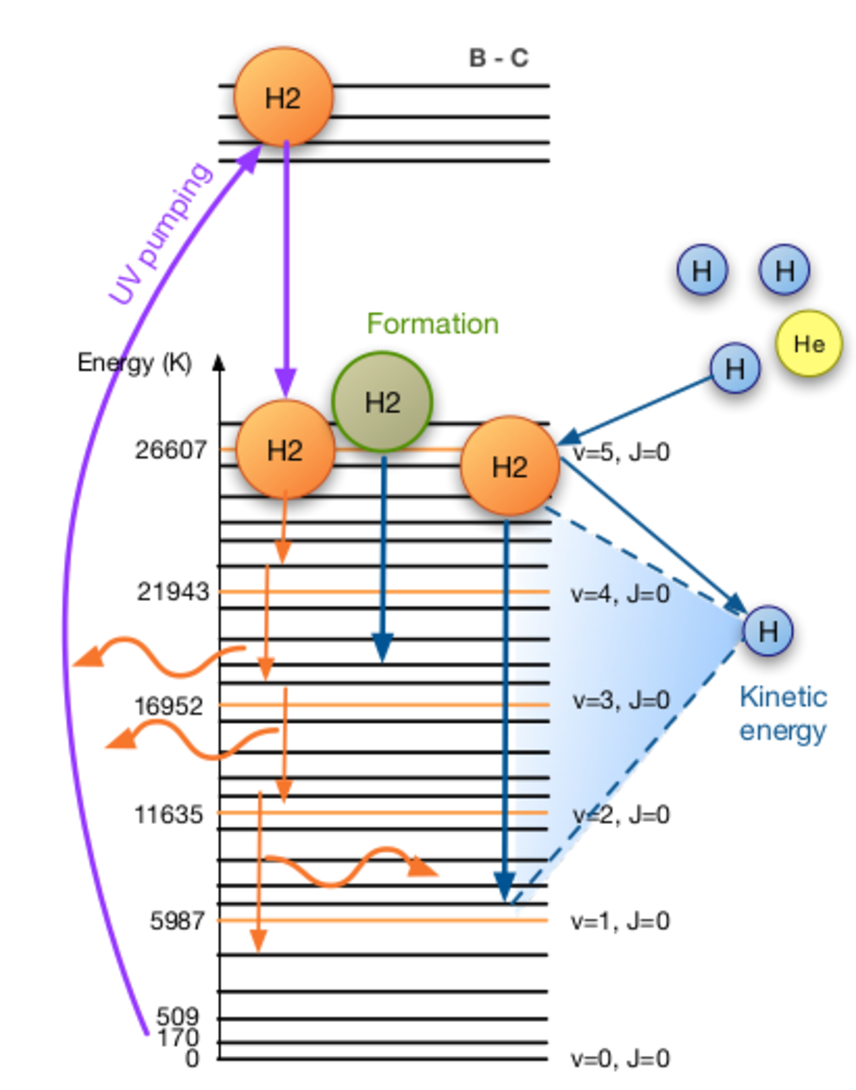
\includegraphics[trim = {0 0 0 0},clip,width=0.6\textwidth]{figure/h2.pdf}
    \caption{Fonctionnement du pompage UV de $\mathrm{H}_2$}
    \begin{minipage}{\textwidth}
L'absorption d'un photon UV passe la molécule dans ses états électroniques excités B-C (transitions de Lyman ou Werner, $ 11<h\nu<13.6\mathrm{eV}$) puis, par émission spontanée, se désexcite dans le continuum vibrationnel dans $10$-$15\%$ des cas, ou bien, dans $85$-$90\%$ des cas, dans un niveau fondamental ro-vibrationellement excité ($\mathrm{J}\geq0$, $\mathrm{v}>0$). La molécule pourra alors se désexciter soit par émission spontanée soit par collisions avec $\mathrm{H}$, $\mathrm{He}$ ou des électrons. 
    \end{minipage}
    \label{fig:H2pump}
\end{figure}



\subsection{Réactions chimiques initiées par $\mathrm{H}_2$}

Certaines réactions chimiques peuvent avoir des barrières d'activation (ou énergies d'activation) qui correspondent à l'énergie qui doit être apporté aux réactifs pour initier une réaction (figure \ref{fig:H2:Ea}). 

\begin{figure}[!h]
    \centering
    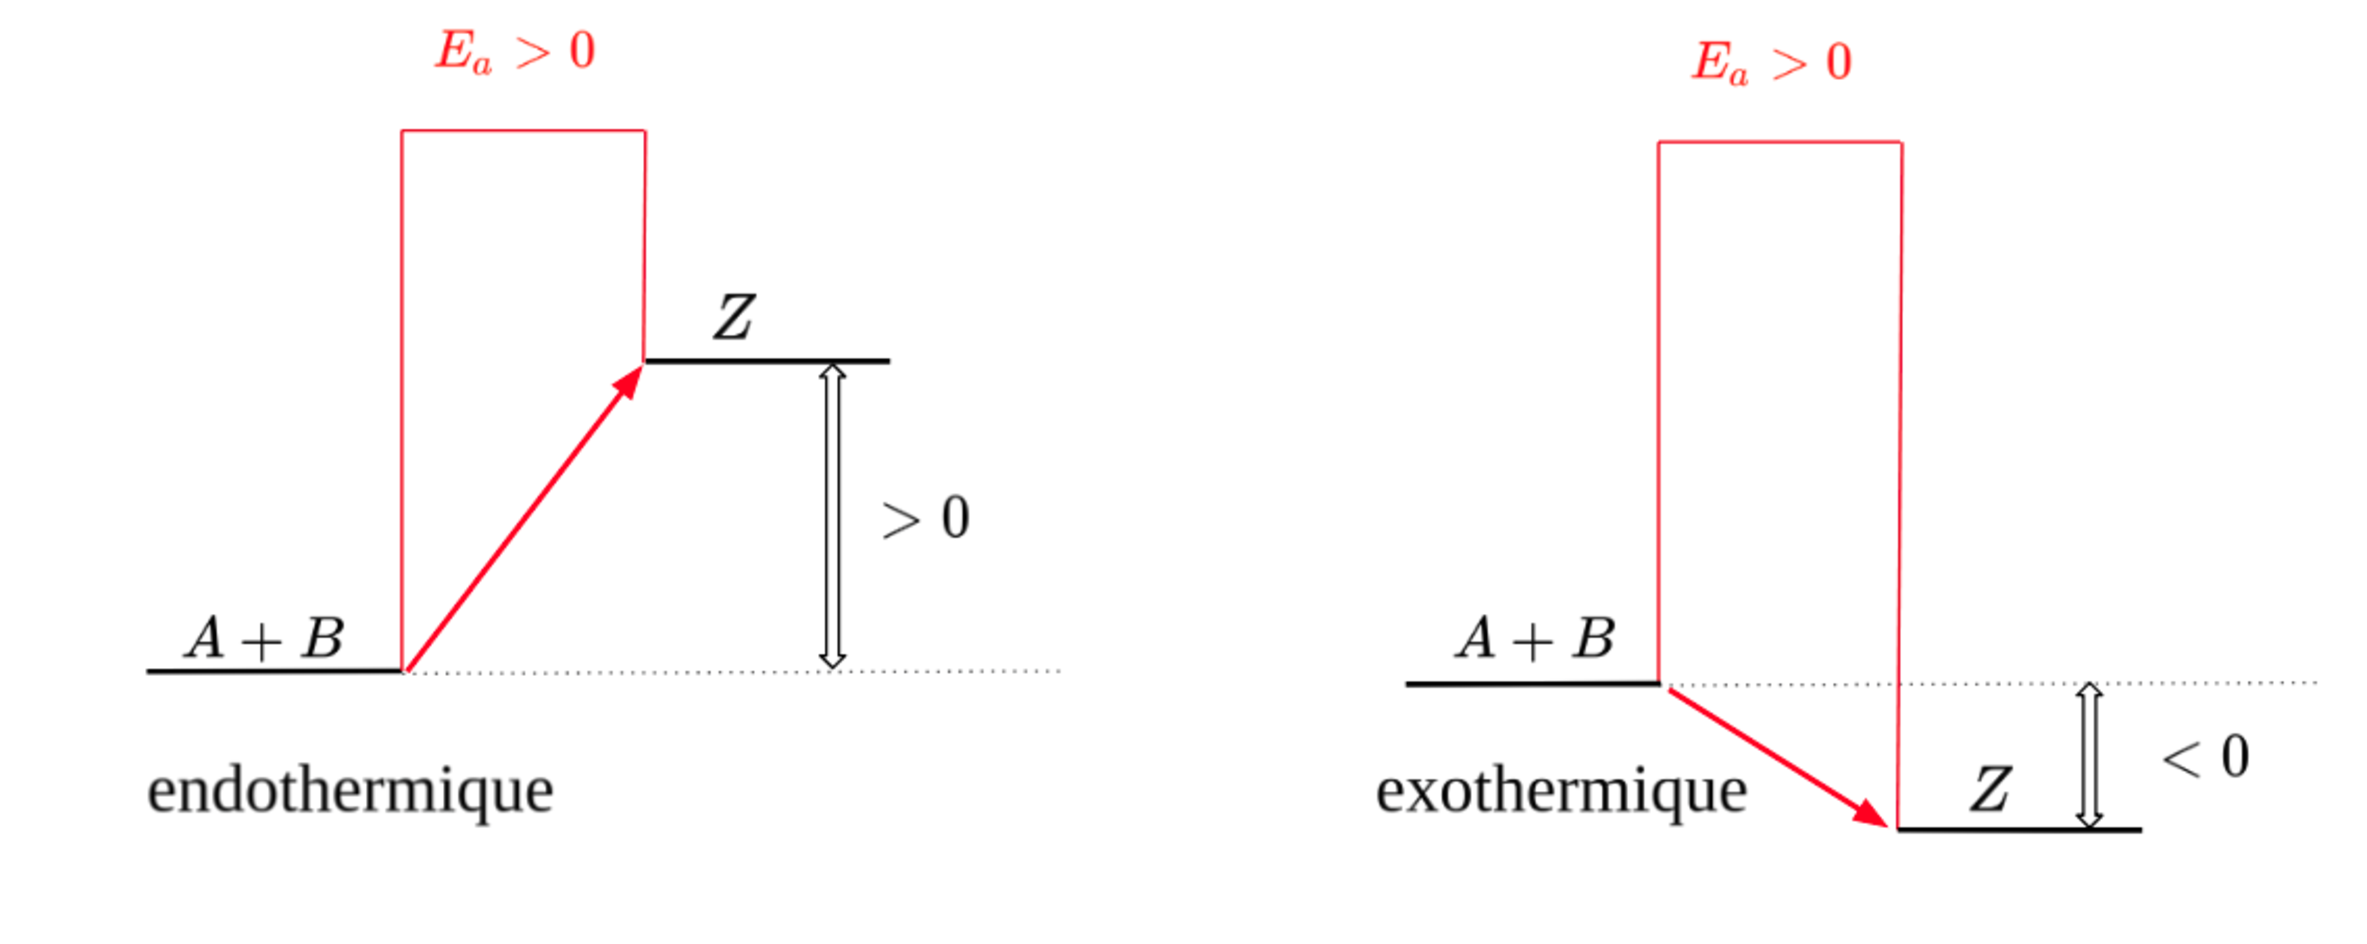
\includegraphics[trim = {0 0 0 0cm },clip,width=0.8\textwidth]{figure/type46/Ea.pdf}
    \caption{Diagramme d'énergie d'une réaction chimique ($\mathrm{A}+\mathrm{B}\rightarrow Z$) ayant une énergie d'activation non nulle}
    \label{fig:H2:Ea}
\end{figure}


Pour passer cette barrière il faut que le gaz soit très chaud ou alors il faut prélever de l'énergie interne des réactifs. De nombreuses réactions permettant la formation de traceurs importants ont une barrière d'activation comme $\mathrm{C}^+ + \mathrm{H}_2 \rightarrow \mathrm{CH}^+ + \mathrm{H}$ ($4537$ K),  $\mathrm{O} + \mathrm{H}_2 \rightarrow \mathrm{OH} + \mathrm{H}$  ($3241$ K) ou bien $\mathrm{N} + \mathrm{H}_2 \rightarrow \mathrm{NH} + \mathrm{H}$ ($16\,607$ K). C'est un phénomène déjà bien connu pour la formation du $\mathrm{CH}^+$ par $\mathrm{H}_2$ \cite{Herraez, Zanchet}. Grâce au pompage UV, la molécule $\mathrm{H}_2$ peut facilement initier les réactions auxquelles elle participe. Il faut alors connaître les taux de réactions états par états des réactifs. Ils sont déjà connus pour $\mathrm{H}_2$ avec $\mathrm{C}^+$ et $\mathrm{H}_2$ et $\mathrm{S}^+$. Pour les autres espèces, il faut calculer un nouveau taux de réaction qui prend en compte l'énergie interne $E_i$ que peut fournir chaque niveaux $i$ de $\mathrm{H}_2$. On obtient un nouveau taux de réaction $k'$ qui est de la forme :

\begin{equation}
    k(T) = A e^{- E_a / k_BT} \quad \rightarrow \quad  k(T)' =  \frac{1}{n_{tot}} \sum_i A_i n_i e^{- (E_a - E_i) / k_BT}
\end{equation}

Ces nouveaux calculs des taux de réactions peuvent potentiellement changer les profils de température des nuages par l'exothermicité ou l'endothermicité des réactions chimiques. Ce n'est pas le cas. Néanmoins, les intensités des raies de traceurs importants comme le $\mathrm{CO}$ (figure \ref{fig:type46:CO}), $\mathrm{H}_2$ (figure \ref{fig:type46:H2}) et $\mathrm{H}_2\mathrm{O}$ (figure \ref{fig:type46:H2O}) sont impactées. Une analyse des réseaux chimiques ont souligné l'importance d'une voie de formation du $\mathrm{CO}$ qui est souvent négligée. Les observations Heschel ont montré que la formation \mathrm{CO} était principalement initiée par celle du $\mathrm{CH}^+$ via $\mathrm{C}^+ + \mathrm{H}_2 \rightarrow \mathrm{CH}^+ + \mathrm{H}$. Or, on a une nouvelle voie de formation principale qui initie celle du $\mathrm{CO}$, il s'agit de $\mathrm{O} + \mathrm{H}_2 \rightarrow \mathrm{OH} + \mathrm{H}$ (le schéma de la figure \ref{fig:type46:form:CO} décrit le réseau chimique de formation du $\mathrm{CO}$). \newline 


D'autres espèces sont impactées par le nouveau calcul des taux de réactions comme $\mathrm{N}$, $\mathrm{HCN}$ ou bien $\mathrm{H}_2\mathrm{O}$ mais l'on n'en discutera pas. Cette étude a permis de mettre à jour la chimie des nuages. Dans les développements futurs, le code PDR intégrera ces nouveaux calculs des taux de formations pour les réactions ayant une barrière d'activation non nulle. 


\begin{figure}[!h]
    \centering 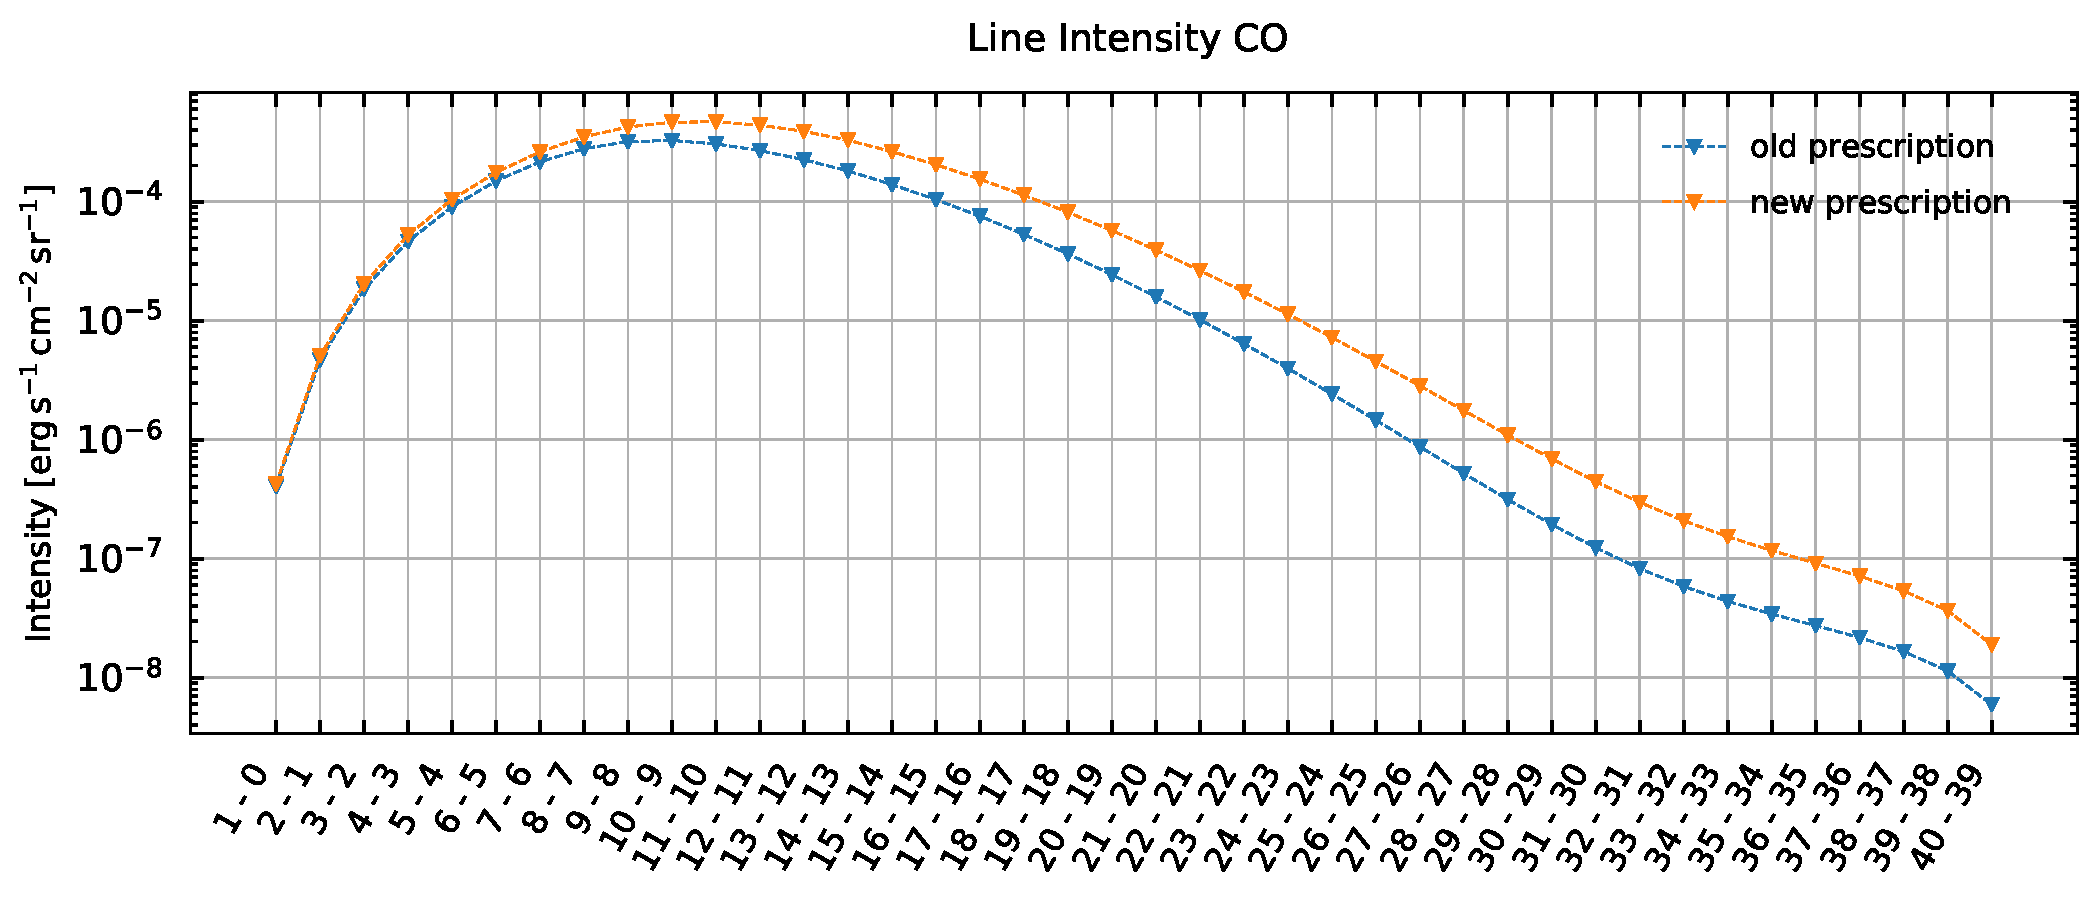
\includegraphics[trim = {0 0 0 1cm},clip,width=0.9\textwidth]{figure/type46/I_comp_CO.pdf}
    \caption{Diagramme d'intensité du $\mathrm{CO}$ avec la nouvelle prescription}
    \begin{minipage}{\textwidth}
    Seules les transitions rotationnelles du $\mathrm{CO}$ ont été écrites (toutes s'effectuent à $\mathrm{v}=0$). On a utilisé un modèle isobare ($\mathrm{P} = 2.8\,10^{8} \,\mathrm{cm}^3\,\mathrm{K}$ et $\chi = 3.1\, 10^4$).
    \end{minipage}
    \label{fig:type46:CO}
\end{figure}

\begin{figure}[!h]
    \centering 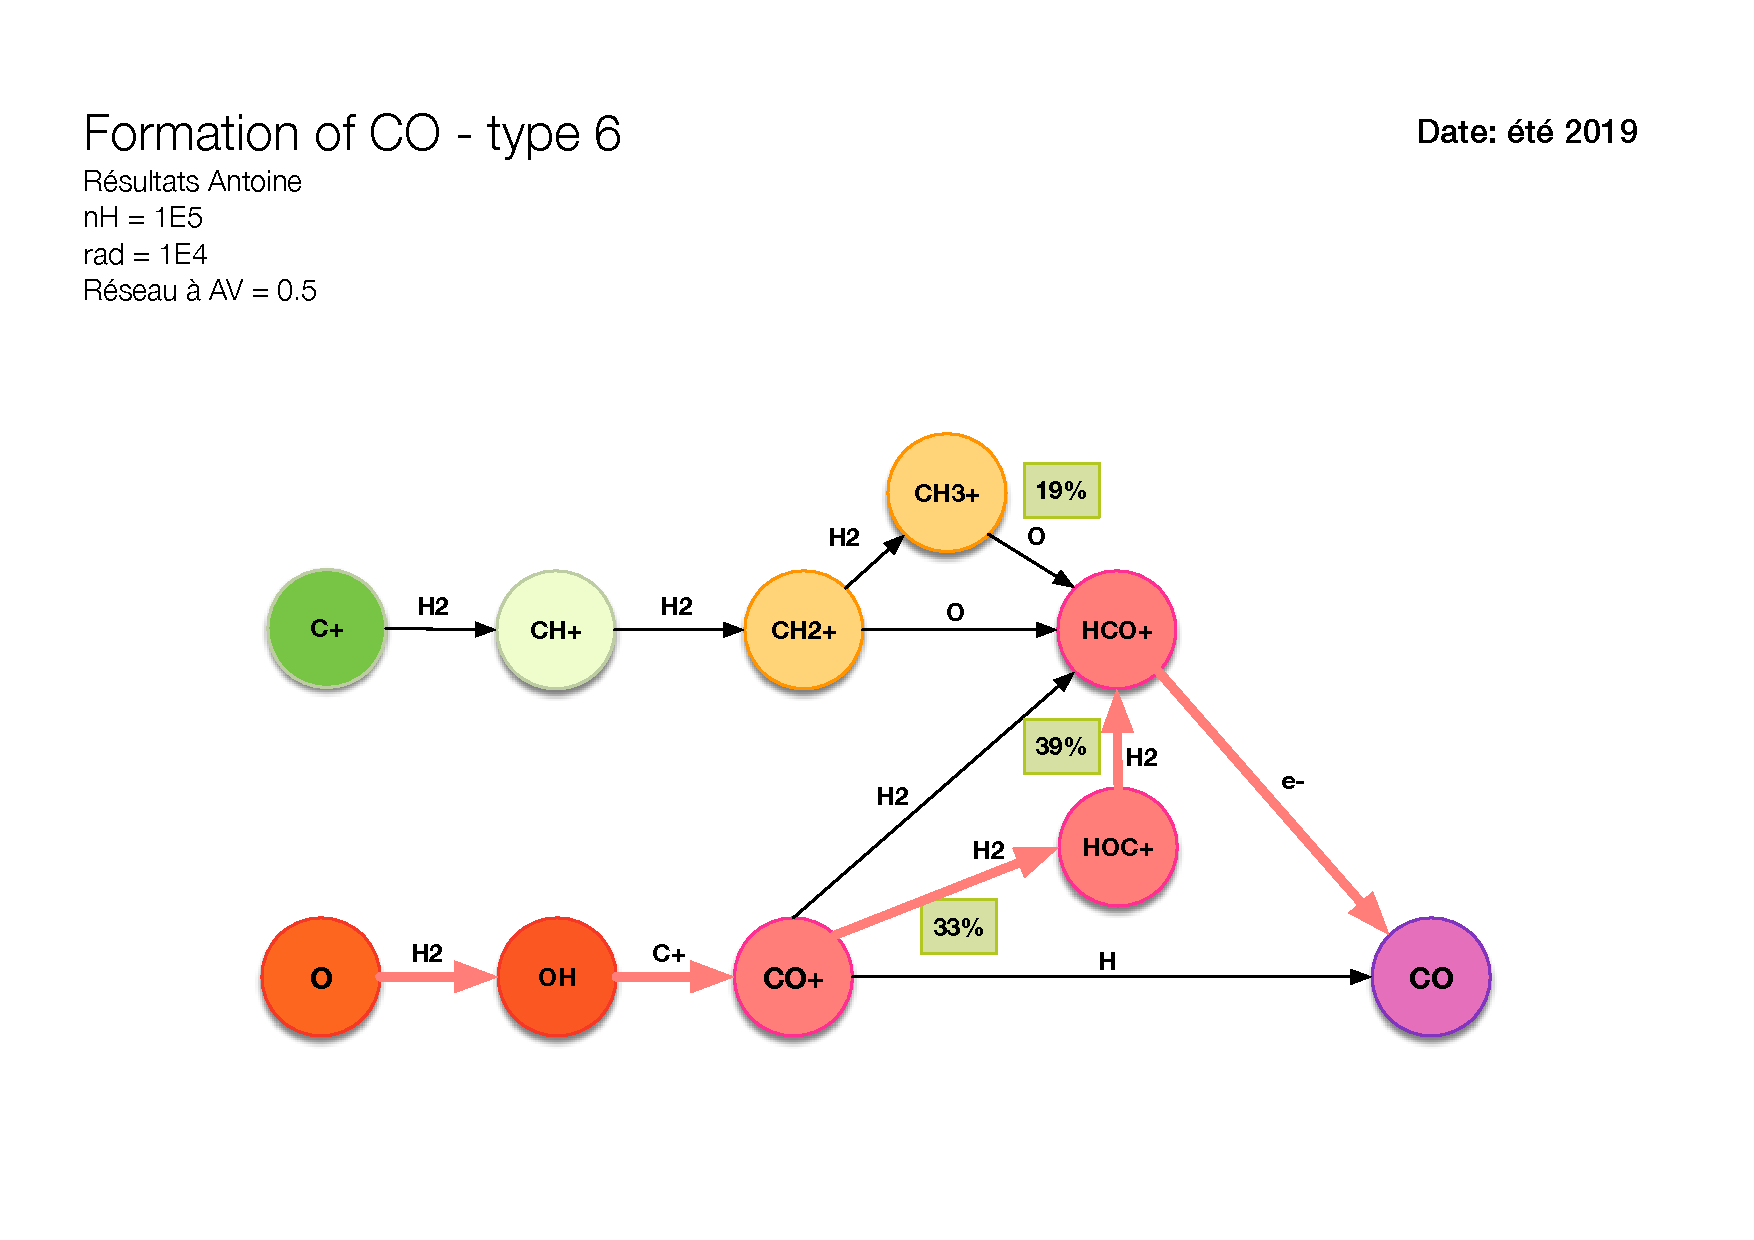
\includegraphics[trim = {3cm 3cm 3cm 7cm},clip,width=0.8\textwidth]{figure/type46/ChimieCO_2.pdf}
    \caption{Nouveau réseau de formation du $\mathrm{CO}$}
    \begin{minipage}{\textwidth}
    A titre de comparaison, l'ancien réseau chimique se trouve en annexe figure \ref{fig:type46:form:COold}.
    \end{minipage}
    \label{fig:type46:form:CO}
\end{figure}

% En comparant les réseaux chimiques du modèle avec la nouvelle prescription on trouve que la réaction $\mathrm{O} + \mathrm{H}_2 \rightarrow \mathrm{OH} +  \mathrm{H}$, devenue efficace, augmente la densité de $\mathrm{H}_2\mathrm{O}$ ($\times 10$) ainsi que ses raies d'émissions (figure \ref{fig:type46:H2O}). On constate également que la réaction $\mathrm{N} + \mathrm{H}_2 \rightarrow  \mathrm{NH} +  \mathrm{H}$ devient importante. La densité du $\mathrm{NH}$ augmente ($\times 10^3$) de même que celle du $\mathrm{HCN}$ ($\times 2$) et de $\mathrm{NO}$ ($\times 2$). Il est présenté dans l'appendice \ref{} les voies de formations des espèces qui sont impactées par le nouveau calcul des taux de réactions.\newline 



% On cherche dans un premiers temps des expressions permettant d'estimer le chauffage par pompage UV de la molécule $\mathrm{H}_2$ calculé par le code. 

% \subsection{Construction d'un modèle}
% \subsubsection{Chauffage net par Rollïg (1995)}

% \subsubsection{Chauffage par désexcitation collisionelle}
% Eq (10) ou (C.3).

% Il propose un modèle d'excitation effectif à deux niveaux au lieu d'un modèle prenant en compte les 15 premiers états vibrationels ($v\leq 15$) de la molécule. Se fonde sur Sternberg&Dalgarno (1995) et Burton (1990). Traduit l'absorption du flux de photons à un taux $P$ (90\% sert à à exciter la molécule) puis le chauffage par désexcitation collisionelle. 
% $\Gamma_{\mathrm{H}_2^\star} > 0$
 
% \begin{equation}
% \Gamma_{\mathrm{H}_2^\star} = n_{\mathrm{H}_2}\frac{\chi P}{1 + \frac{A_{\text{eff}}+ \chi D_{\text{eff}}}{\gamma_{\text{eff}}\, n}} \Delta E \operatorname{erg} \mathrm{cm}^{-3} \mathrm{s}^{-1}
% \end{equation}

% Où le taux de pompage par unité de champs FUV $P = 2 \times 2.9\,10^{-10}\,\mathrm{s}^{-1}$. Le facteur 2 est considéré car Rollig considère un demi champs incident en bord de nuage (contrairement à nous qui utilisons le flux calculé à partir du transfert radiatif total). Le taux de pompage représente $100\%$ du pompage. Normalement $85$-$90\%$ du pompage maintient la molécule dans un état excité, les autres desexcitation dissocient la molécule. Il retranche un terme de refroidissement pour corriger.

% \subsubsection{Refroidissement par émission de photons}

% Eq (11) ou (C.2).
% Excitation collisonelle (à $v=1$) puis émission (ou photodissociation à inspecter : pourquoi il prend en compte l). Rollïg veut un terme de refroidissement et construit le taux tel que $\Lambda_{\mathrm{H}_2} < 0$.

% \begin{equation}
%     \Lambda_{\mathrm{H}_2} = - \Delta E_{1,0} \, \gamma_{1,0} e^{-\Delta E_{1,0}/kT} n_{\mathrm{H}} \, n_{\mathrm{H}_2} \frac{A_{1,0} + \chi D_1}{\gamma_{1,0}  n_{\mathrm{H}} + A_{1,0} + \chi D_1} \operatorname{erg} \mathrm{cm}^{-3} \mathrm{s}^{-1}
% \end{equation}

% \subsubsection{Bialy et Sternberg (2019)}
% \subsubsubsection{Chauffage par désexcitation collisionelle}

% \cite{BialySternberg_2019} (A12) considère que 9 photons sur 10 permettent d'avoir du $\mathrm{H}_2$ excité. 

% \begin{equation}
%     \Gamma_{\mathrm{H}_2 \, \mathrm{pump}} = 9D_0 \chi \, E_{\mathrm{pump}} \, n(\mathrm{H}_2) \times \frac{1}{1 + \frac{n_{\mathrm{crit}}}{n_\mathrm{H}} } \operatorname{erg} \mathrm{cm}^{-3} \mathrm{s}^{-1}
% \end{equation}

% $D_0$ est le taux de photodissociation ($P \approx 10 D_0$, 1 photon sur 10 mène à une photodissociation). $E_{\mathrm{pump}} = 1.12\,eV$ et $n_{\mathrm{crit}} = 1.1\,10^5 /\sqrt{T/1000\mathrm{K}} \, \mathrm{cm}^{-3}$ représente la compétition entre émission spontanée et désexcitation par collisions. Si on compare ces termes entre \cite{BialySternberg_2019} et \cite{Rollig2005} au bord de nuage avec un champs de rayonnement $\chi = 10^5 $

% \begin{equation}
%     \frac{A_{\text{eff}}+ \chi D_{\text{eff}}}{\gamma_{\text{eff}}} \approx 2.9\,10^{6} /\sqrt{T/1000\mathrm{K}} \, \mathrm{cm}^{-3} \quad !\sim n_{\mathrm{crit}}
% \end{equation}

% \subsubsection{Chauffage par photodissociation}

% \begin{equation}
%     \Gamma_{\mathrm{H}_2 \, \mathrm{pd}} = D_0\,\chi \, E_\mathrm{pd} \, n(\mathrm{H}_2)
% \end{equation}

% \subsubsection{Absorption du rayonnement}
% \subsubsubsection{Shielding par le molécule $\mathrm{H}_2$}

% On utilise la fonction fitté (Eq.37) par \cite{DraineBertoldi_1996} pour calculer le \textit{shielding} de la molécule $\mathrm{H}_2$ sur le taux d'excitation par pompage $\chi P$.

% $$
% f_{\text {shield}}\left(x\right)=\frac{0.965}{\left(1+x / b_{5}\right)^{2}}+\frac{0.035}{(1+x)^{0.5}} \exp \left[-8.5 \times 10^{-4}(1+x)^{0.5}\right]
% $$

% avec $x = N(\mathrm{H}_2)/5\,10^{14} \, \mathrm{cm}^{-2}$ et $b_5 = b/10^5 \, \mathrm{cm}\,\mathrm{s}^{-1}$. L'écrantage affecte la formation et destruction de la molécule. Je multiplie la fonction $f_{\text {shield}}$ au champs de rayonnement $\chi$.
% On obtient ainsi un nouveau taux de chauffage :

% \begin{equation}
%     \Gamma_{\mathrm{H}_2^\star} = n_{\mathrm{H}_2}\frac{\chi P \, f_{\text {shield}}}{1 + \frac{A_{\text{eff}}+  f_{\text {shield}} \chi D_{\text{eff}}}{\gamma_{\text{eff}} \, n}} \Delta E \operatorname{erg} \mathrm{cm}^{-3} \mathrm{s}^{-1}
% \end{equation}



% On fait de même pour le taux de refroidissement.

% % \begin{figure}[h!]
% %     \centering
% %     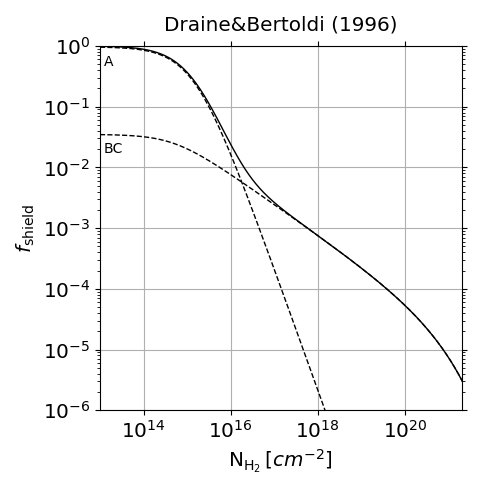
\includegraphics[width = 0.4\textwidth]{figure/H2/pumpingH2/fshield.png}
% %     \caption{Fonction de shielding $f_\mathrm{shield}$ de $\mathrm{H}_2$ en fonction de la colonne densité $N(\mathrm{H}_2)$}
% %     \label{fig:H2:fshield}
% % \end{figure}


% \subsubsection{Extinction par les grains}

% Le champs de rayonnement calculé par le code ne prend pas en compte l'extinction par les grains. Approximation FGK. Je corrige le champs de rayonnement par $e^{-\tau_d}$ où $\tau_d = N_\mathrm{H}\sigma_d$ donné par \cite{SternbergLePetit2014} Eq 20. Ainsi, 

% $$\chi^{'} = e^{-\tau_d
% }\, f_{\mathrm{shield}}\, \chi$$


% \subsubsection{Comparaison avec le code PDR de Meudon}

% On récupère du code le taux de refroidissement $\Lambda_{\mathrm{PDR}}$ par la molécule $\mathrm{H}_2$ qui peut être positif ou négatif. Le taux prend en compte du chauffage par desexcitation collisionnelle et du refroidissement ro-vibrationelle (émission). Il ne prend pas en compte de la photodissociation (qui chauffe). On veut étudier le chauffage, on appelle $\Gamma_{\mathrm{PDR}}$ la partie négative du taux ($\Lambda_{\mathrm{PDR}} < 0$) et on le compare aux de chauffage nets.

% \begin{equation}
%     \begin{split}
%         \Gamma_{\mathrm{Rollig} \, \mathrm{net}} &= \Gamma_{\mathrm{H}_2^\star} + \Lambda_{\mathrm{H}_2} \\ 
%         \Gamma_{\mathrm{BS} \, \mathrm{net}} &=\Gamma_{\mathrm{H}_2 \, \mathrm{pump}} +  \Gamma_{\mathrm{H}_2 \, \mathrm{pd}} 
%     \end{split}
% \end{equation}

% La figure \ref{fig:H2:GammaPDR} compare les taux de chauffages nets utilisant différentes prescriptions à celui calculé dans le code (en noir). Le chauffage calculé par Rollïg et de Bialy\&Sternberg ont la même intensité en bord de nuage où la désexcitation collisionnelle est prédominante. 

% L'approximation FGK est une méthode qui calcule le spectre du champs de rayonnements à travers le nuage qui prend en compte l'absorption dans le continuum et le carbone. Il prend également en compte l'écrantage de la molécule $\mathrm{H}_2$ (figure \ref{fig:H2:fgk} \cite{FGK}). 

% \begin{figure}[h!]
%     \centering
%     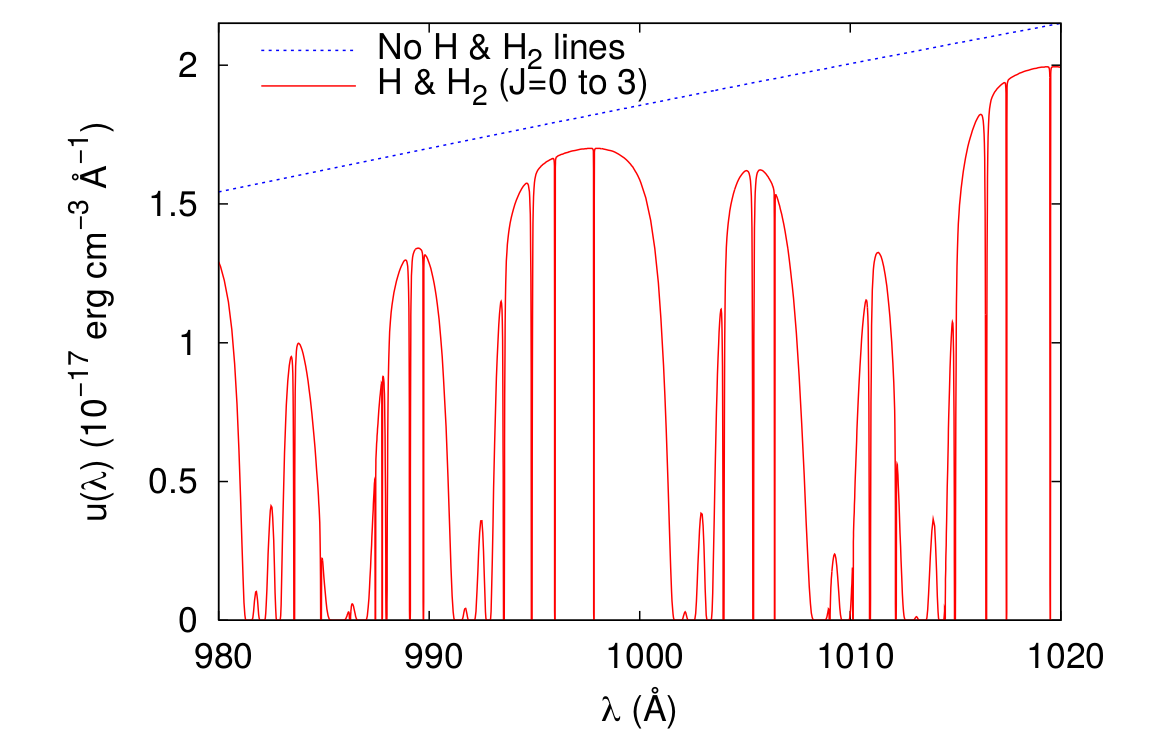
\includegraphics[width = 0.6\textwidth]{figure/H2/fgk.png}
%     \caption{Densité d'énergie au sein d'un nuage à un $A_\mathrm{V}=0.5$. Les niveaux du $\mathrm{H}$ et de $\mathrm{H}_2$ absorbent certains photons sur certaines raies. A mesure que l'on s'enfonce dans le nuage beaucoup de matière se trouve sur la ligne de visée et les raies d'absroptions s'élargissent (voir optiquement épaisse Draine) \cite{FGK}}
%     \label{fig:H2:fgk}
% \end{figure}

%%%%%%%%%%%%%%%%%%%%%%%%%%%%%%%%%%%%%%%%%%%%%%%%%%%%%%%%%%%%%%%%%%%%%%%%%%%%%

\subsection{Dissociation collisionelle du $\mathrm{H}_2$}

Une autre voie de destruction rapide du $\mathrm{H}_2$ autre que la photodissociation est la dissociation collisionnelle (eq. \ref{eq:H2diss}). Les taux de réaction de ces voies sont mal connues et jouent dans les bords atomiques des nuages où la température est élevée. 

\begin{equation}\label{eq:H2diss}
    \begin{array}{lcccccccl}
        \mathrm{H} & + & \mathrm{H}_2   & \rightarrow &\mathrm{H}  & + & \mathrm{H} & + & \mathrm{H} \\
        \mathrm{H}_2  & + & \mathrm{H}_2  & \rightarrow & \mathrm{H} & + &\mathrm{H}_2  & + & \mathrm{H} \\
    \end{array}
\end{equation}

Il existe plusieurs prescriptions qui tentent d'estimer ces taux en fonction de la température. Deux ont été retenu dans le code : celle de Glover et Mac Low \cite{GloverMacLow_2007} et celle de Janev \cite{Janev2003}. On constate par ailleurs que la prescription de Glover obtient des taux de dissociation plus faibles devant ceux de Janev ce qui peut changer radicalement la composition du nuage. Nous avons étudié les modifications qu'apportaient la prescription de Glover par rapport à Janev puis avons choisi de garder celle qui correspondait le mieux aux observations.


\subsubsection{Grilles de modèles - Bord atomique}

Sur la figure \ref{fig:H2:JanevGlover:Tba}, la température en bord de nuage atomique est représentée. On constate qu'elle est sensiblement similaire selon que l'on utilise la prescription de Janev ou de Glover à l'exception des PDR denses et fortement illuminées ($n_\mathrm{H} \geq 10^{4.5} \, \mathrm{cm}^{-3}$ et $\chi \geq 10^3$) qui sont légèrement plus chaudes. En visualisant sur la figure \ref{fig:H2:JanevGlover:diffTba} la différence des cartes de température, on comprend que la prescription de Glover a tendance à chauffer les bords atomiques de l'ensemble des PDR de $+200$ K et peut augmenter la température jusqu'à $+800$ K pour les PDR denses et fortement illuminées. \newline

\begin{figure}[!h]
    \centering 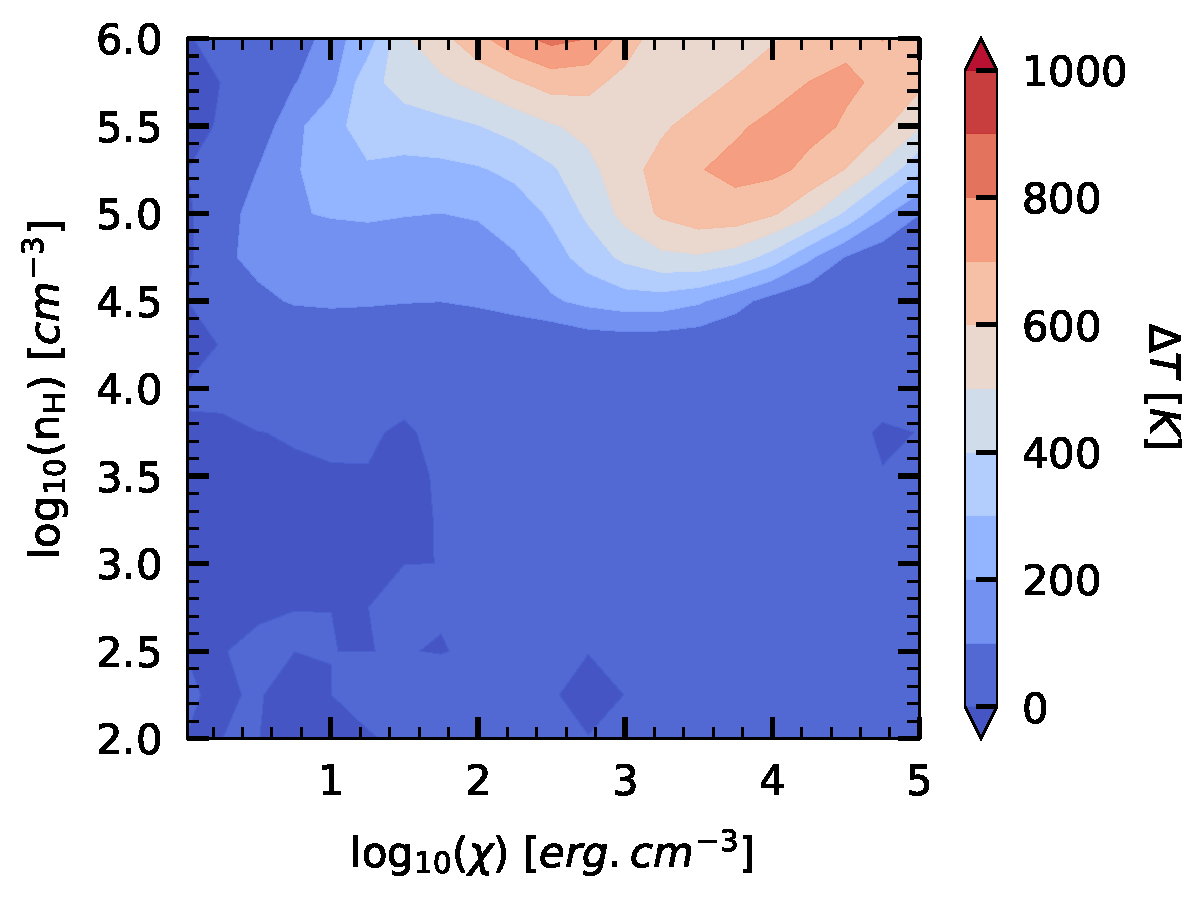
\includegraphics[trim = {0 0 0 0 },clip,width=0.6\textwidth]{figure/H2/diffgrid_gloverjanev/mapTba_H2_n_1p7_nobossion_noCl155_n.pdf}
    \caption{Différence de température aux bords de nuage entre des modèles utilisant la prescription de Janev et de Glover}
    \label{fig:H2:JanevGlover:diffTba}
\end{figure}

Cette différence est due à l'amélioration du chauffage par la molécule $\mathrm{H}_2$. La prescription de Glover diminue les taux de destruction ce qui produit davantage de $\mathrm{H}_2$ dans le bord atomique. Le chauffage étant d'autant plus efficace que la densité de $\mathrm{H}_2$ est grande, les bords atomiques de l'ensemble des PDR chauffent. Par ailleurs, le chauffage par $\mathrm{H}_2$ devient particulièrement efficace dans les régions denses et fortement illuminées. \newline

On constate sur la figure \ref{fig:H2:JanevGlover:Gmax} que le chauffage par $\mathrm{H}_2$ reste dominant dans les bords atomique des PDR denses quelque soit la prescription que l'on utilise. En revanche, les processus de refroidissement (figure \ref{fig:H2:JanevGlover:Lmax}) varient pour les PDR denses et faiblement illuminées ($n_\mathrm{H} \geq 10^{4.5} \, \mathrm{cm}^{-3}$ et $\chi \leq 10^3$). Les réactions de dissociations collisionnelles sont des réactions endothermiques efficaces. Le changement de prescription diminue les taux de réaction et donc les taux de refroidissement par ces réactions. 


%%%%%%%%%%%%%%%%%%%%%%%%%%%%%%%%%%%%%%%%%%%%%%%%%%%%%%%%%%%%%%%%%%%%%%%%%%%%%%
\subsubsection{Grilles de modèles - Transition $\mathrm{H}/\mathrm{H}_2$}

La transition $\mathrm{H}/\mathrm{H}_2$ marque la frontière entre le milieu atomique et moléculaire du nuage. Elle survient une fois que le $\mathrm{H}_2$, jusque là détruit dans la zone atomique par les photons UV, parvienne à se former en suffisamment grande quantité pour que l'hydrogène soit majoritairement sous forme moléculaire. Nous avons définit le critère tel qu'il y ait autant d'élément hydrogène sous forme atomique que moléculaire soit $n(\mathrm{H}) = 2 n(\mathrm{H}_2)$. La température et l'$\mathrm{A}_\mathrm{v}$ auxquelles s'effectuent la transition $\mathrm{H}/\mathrm{H}_2$ sont déterminants puisque les observables moléculaires se forment et sont excitées dans cette région du nuage qui est encore chaude. \newline

Les figures \ref{fig:H2:JanevGlover:THH2} et \ref{fig:H2:JanevGlover:AVHH2} montrent les températures et les $\mathrm{A}_\mathrm{v}$ des transitions de chaque modèles. Alors que la position de la transition dans le nuage reste sensiblement identique (figure \ref{fig:H2:JanevGlover:AVHH2}) en passant de la prescription de Janev à celle de Glover, la température parvient à dépasser un plateau à $600$ K et atteint les $1000$ K (figure \ref{fig:H2:JanevGlover:THH2}). Ce résultat peut avoir un impact important sur les diagrammes d'intensités des traceurs. 

% \begin{figure}[!h]
%     \centering 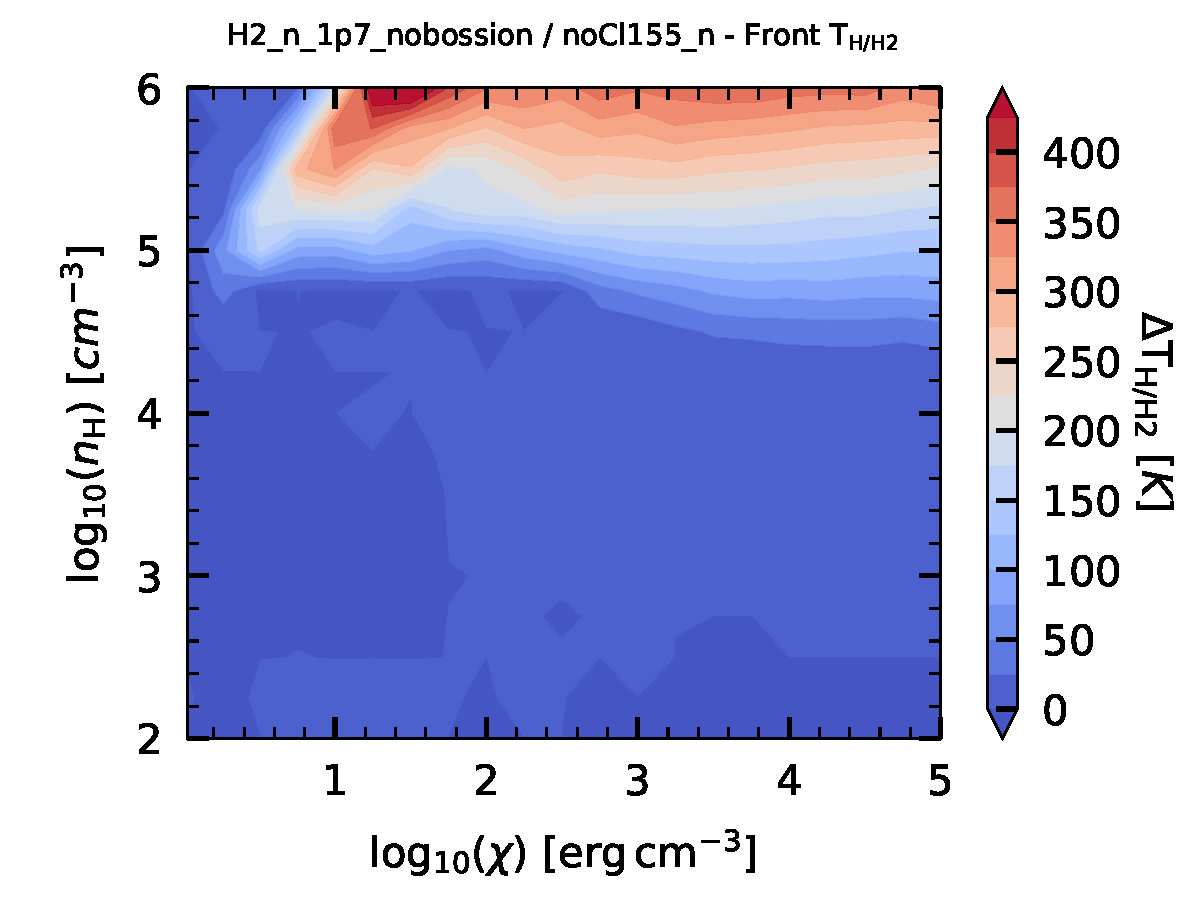
\includegraphics[trim = {0 0 0 1cm },clip,width=0.6\textwidth]{figure/H2/diffgrid_gloverjanev/HH2_T_H2_n_1p7_nobossion_noCl155_n.pdf}
%     \caption{Différence de température à la transition $\mathrm{H}/\mathrm{H}_2$ entre des modèles utilisant la prescription de Janev et de Glover}
%     \label{fig:H2:JanevGlover:diffTHH2}
% \end{figure}

\begin{figure}[!h]
    \centering
    \begin{subfigure}[t]{0.49\textwidth} % "0.49" donne ici la largeur de l'image
        \centering 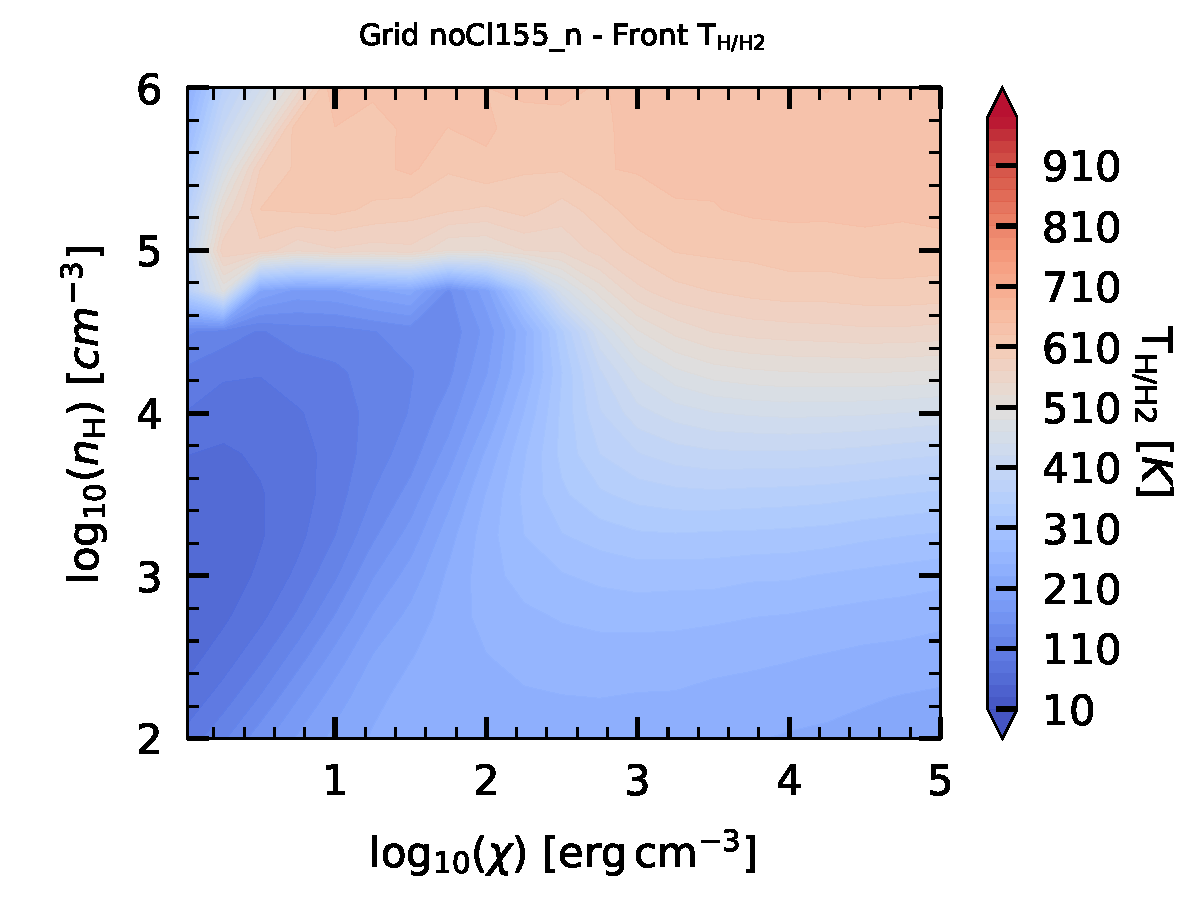
\includegraphics[trim = {0 0 0 1cm },clip,width=1\textwidth]{figure/H2/grid_janev/HH2_T.pdf}
        \caption{Prescription de Janev}
    \end{subfigure}
    ~ 
    \begin{subfigure}[t]{0.49\textwidth}
        \centering 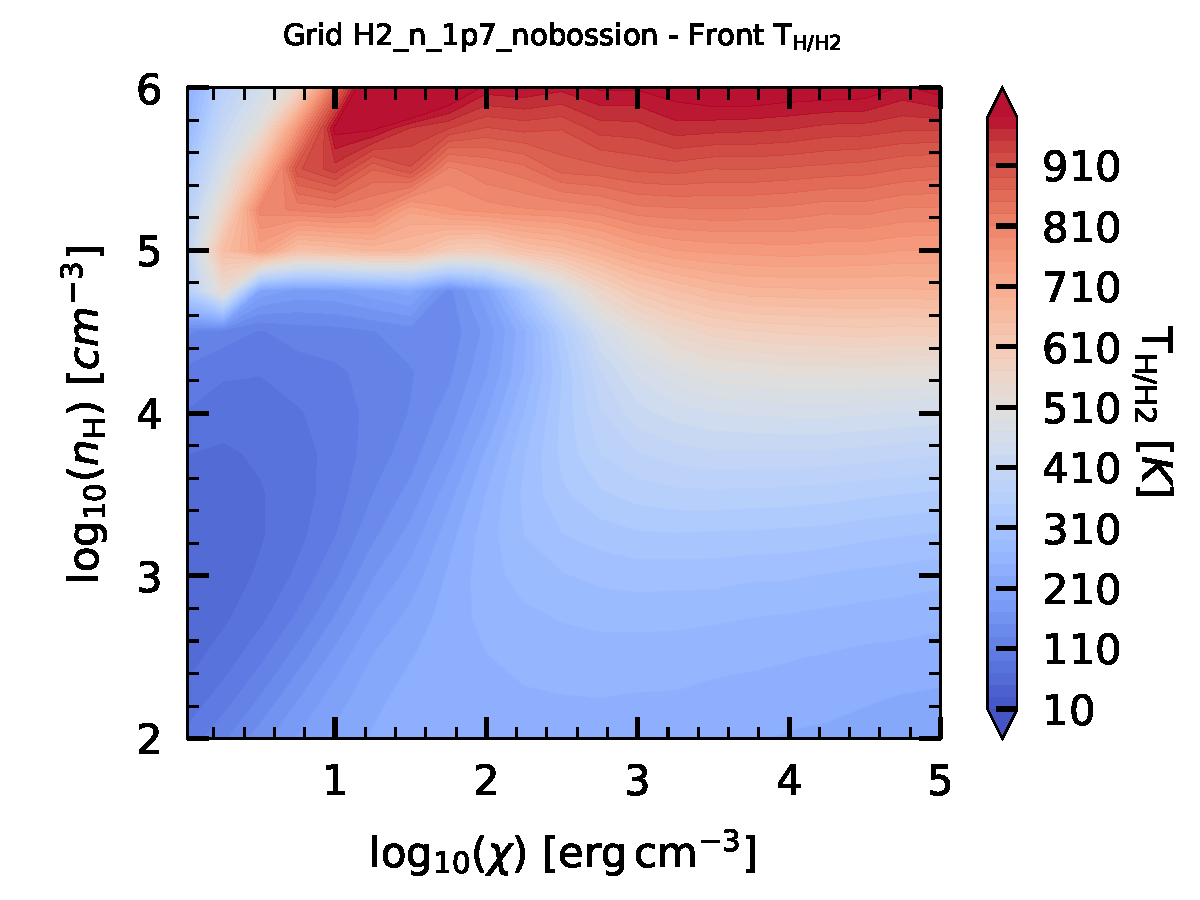
\includegraphics[trim = {0 0 0 1cm },clip,width=1\textwidth]{figure/H2/grid_glover/HH2_T.pdf}
        \caption{Prescription de Glover}
    \end{subfigure}
    \caption{Comparaison de la température à la transition $\mathrm{H}/\mathrm{H}_2$ des modèles utilisant la prescription de Janev et de Glover}
    \label{fig:H2:JanevGlover:THH2}
\end{figure}

 
%%%%%%%%%%%%%%%%%%%%%%%%%%%%%%%%%%%%%%%%%%%%%%%%%%%%%%%%%%%%%%%%%%%%

\subsubsection{Étude d'un modèle particulier}

On cherche à comprendre dans cette section d'où vient l'augmentation de la température à la transition $\mathrm{H}/\mathrm{H}_2$. On a choisit un modèle à $n_\mathrm{H} = 10^{5.5} \,\mathrm{cm}^{-3}$ et $\chi = 10^4$ qui subit une augmentation de $+300$ K à la frontière. Le profil de température (figure \ref{fig:H2:bosse:plotH}) montre une augmentation locale de la température commençant à un $\mathrm{A}_\mathrm{v} \approx 0.1 \,\mathrm{mag}$ et finissant à $\mathrm{A}_\mathrm{v} \approx 0.4 \,\mathrm{mag}$ accompagnée d'une augmentation de la densité de $\mathrm{H}_2$. L'augmentation locale de température est également très proche de la transition $\mathrm{C}^+/\mathrm{C}/\mathrm{CO}$ permettant de former du $\mathrm{CO}$ chaud. \newline 

\begin{figure}[!h]
    \centering
    \begin{subfigure}[t]{0.49\textwidth} % "0.49" donne ici la largeur de l'image
        \centering 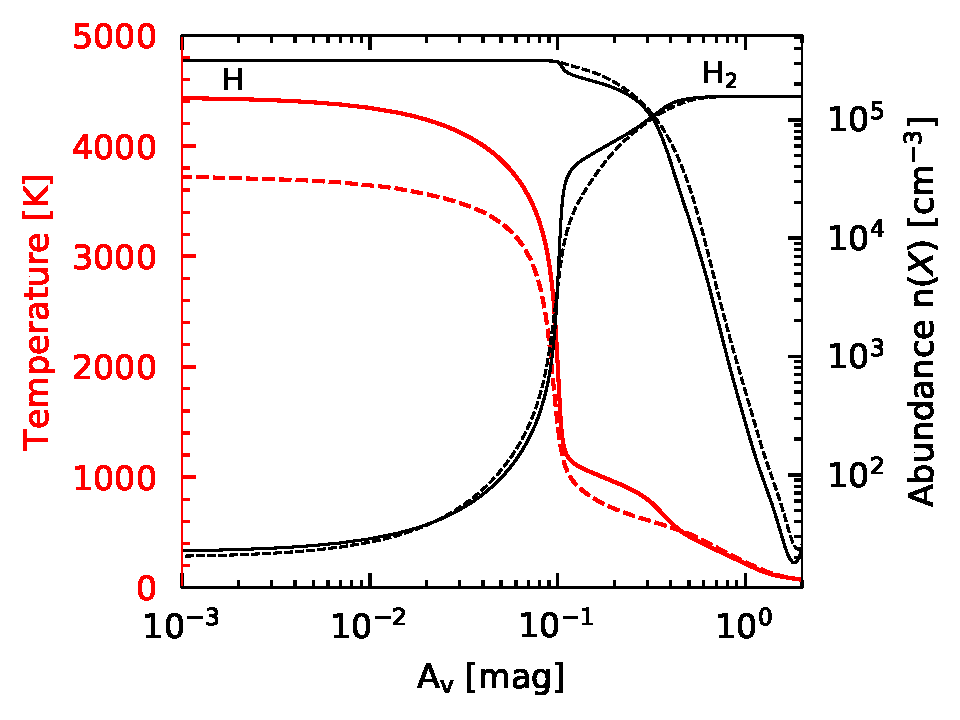
\includegraphics[trim = {0 0 0 0 },clip,width=1\textwidth]{figure/H2/bosse_dcte_janevVSglover/profilT.pdf}
        \caption{}
        \label{fig:H2:bosse:plotH}
    \end{subfigure}
    \begin{subfigure}[t]{0.49\textwidth}
        \centering 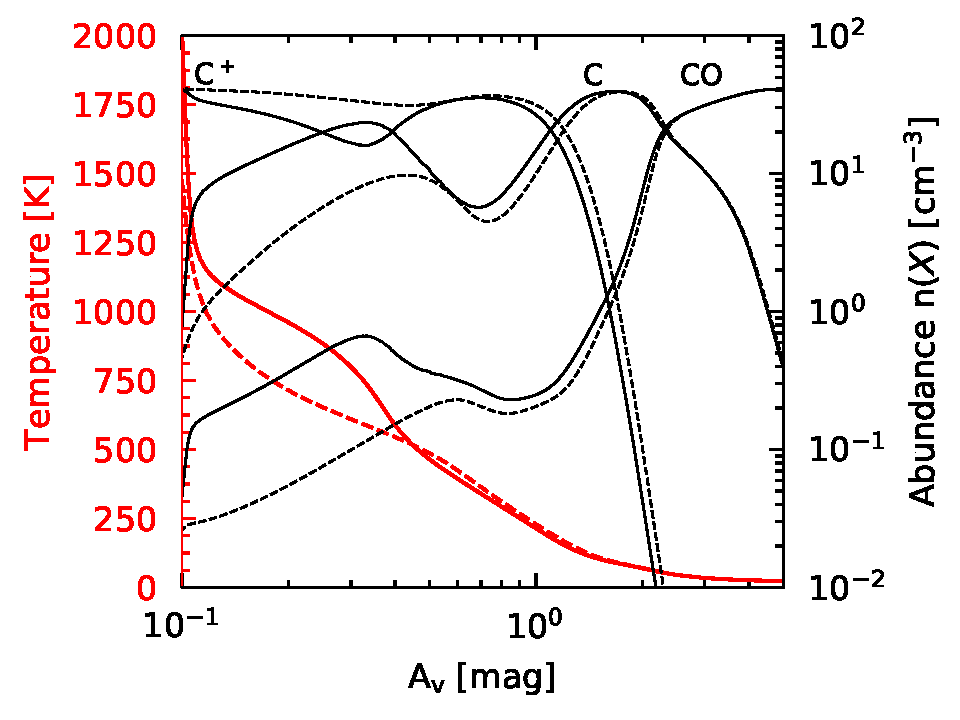
\includegraphics[trim = {0 0 0 0 },clip,width=1\textwidth]{figure/H2/bosse_dcte_janevVSglover/Cp_C_CO.pdf}
        \caption{}
    \label{fig:H2:bosse:plotC}
    \end{subfigure}
    \caption{Profils de densités de $\mathrm{H}$ et $\mathrm{H}_2$ (a) et $\mathrm{C}^+$, $\mathrm{C}$ et $\mathrm{CO}$ (b) d'un modèle à densité constante ($n_\mathrm{H} = 10^{5.5}\,\mathrm{cm}^{-3}$ et $\chi = 10^4$). Le trait plein correspond au calcul utilisant la prescription de Glover et les trait pointillés celle de Janev. La température est représentée en rouge.}
    
\end{figure}

La figure \ref{fig:H2:bosse:heat} trace les taux de chauffages en fonction de l'extinction. On constate, qu'avec la prescription de Glover, les réactions chimiques chauffent le gaz de manière aussi intense que l'effet photoélectrique ce qui est peu commun dans les PDR. Afin de comprendre l'origine de cette augmentation locale de température, on a tracé à $\mathrm{A}_\mathrm{v} \approx 0.2 \,\mathrm{mag}$, les courbes de chauffage et de refroidissement en fonction de la température (figure \ref{fig:H2:bosse:chem}). L'équilibre thermique du gaz est déterminée par l'intersection de la courbe de chauffage et de refroidissement total. A première vue, les allures des courbes sont très différentes. En passant de la prescription de Janev à celle de Glover, on voit qu'un nouveau processus de chauffage intervient entre $100$ K et $1000$ K. Il s'agit des réactions chimiques qui se mettent à chauffer le gaz de manière plus efficace. \newline

Une analyse préliminaire a montré que le caractère exothermique ou endothermique des réactions chimiques était globalement gouverné par la compétition entre la recombinaison électronique du $\mathrm{CH}_3^+$ (qui est exothermique et qui peut se faire sous quatre formes) et la dissociation collisionnelle du $\mathrm{H}_2$ (qui est endothermique). Les réactions et leurs enthalphies de réactions ont été écrites ci dessous. Le passage de la prescription de Janev à celle de Glover a pour effet d'affailblir la destruction du $\mathrm{H}_2$ ce qui rend le bilan des réactions chimiques exothermique. Il permet également de former plus facilement du $\mathrm{H}_2$ qui devient alors un agent refroidissant efficace. On le visualise sur la figure \ref{fig:H2:bosse:heat}. \newline


\begin{equation}
     \mathrm{CH}_3^+ +  \mathrm{e}^- \rightarrow \left\{ 
    \begin{array}{lcccclr}
         \mathrm{H} &+& \mathrm{CH}_2  & & & \qquad \Delta H_r = - 5.0\,10^2 \,\mathrm{kJ}\,\mathrm{mol}^{-1}\\
         \mathrm{H}_2 &+& \mathrm{CH}  & & & \qquad \Delta H_r = - 5.1\,10^2 \,\mathrm{kJ}\,\mathrm{mol}^{-1}\\
         \mathrm{H} &+& \mathrm{H}_2 &+& \mathrm{C}  & \qquad \Delta H_r = - 1.7\,10^2 \,\mathrm{kJ}\,\mathrm{mol}^{-1}\\
         \mathrm{H} &+& \mathrm{CH} &+& \mathrm{H} & \qquad  \Delta H_r = - 8.0\,10^1 \,\mathrm{kJ}\,\mathrm{mol}^{-1}
    \end{array}\right.
\end{equation}


\begin{equation}
    \begin{array}{lcccccccll}
        \mathrm{H} & + & \mathrm{H}_2   & \rightarrow &\mathrm{H}  & + & \mathrm{H} & + & \mathrm{H} & \Delta H_r = 4.3\,10^{2}\,\mathrm{kJ}\,\mathrm{mol}^{-1} \\
        \mathrm{H}_2  & + & \mathrm{H}_2  & \rightarrow & \mathrm{H} & + &\mathrm{H}_2  & + & \mathrm{H} & \Delta H_r = 4.3\,10^2\,\mathrm{kJ}\,\mathrm{mol}^{-1} \\
    \end{array}
\end{equation}

% L'augmentation de l'intensité des raies se comprend On constate également sur la figure $\ref{fig:H2:bosse:plotC}$ qui représente la transition $\mathrm{C}^+/\mathrm{C}/\mathrm{CO}$ que l. La prescription de Glover permet la formation de $\mathrm{CO}$ chaud 



\begin{figure}[!h]
    \centering
    \begin{subfigure}[t]{0.49\textwidth} % "0.49" donne ici la largeur de l'image
        \centering 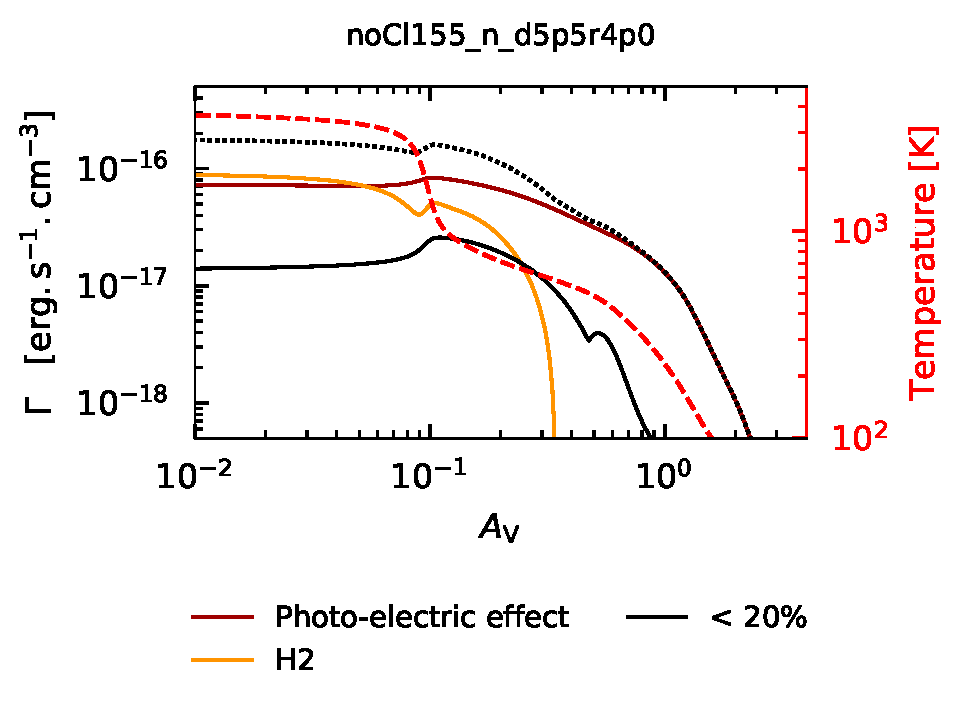
\includegraphics[trim = {0 0 0 1cm },clip,width=1\textwidth]{figure/H2/bosse_dcte_janevVSglover/janev/heat.pdf}
        \caption{Prescription de Janev}
    \end{subfigure}
    \begin{subfigure}[t]{0.49\textwidth}
        \centering 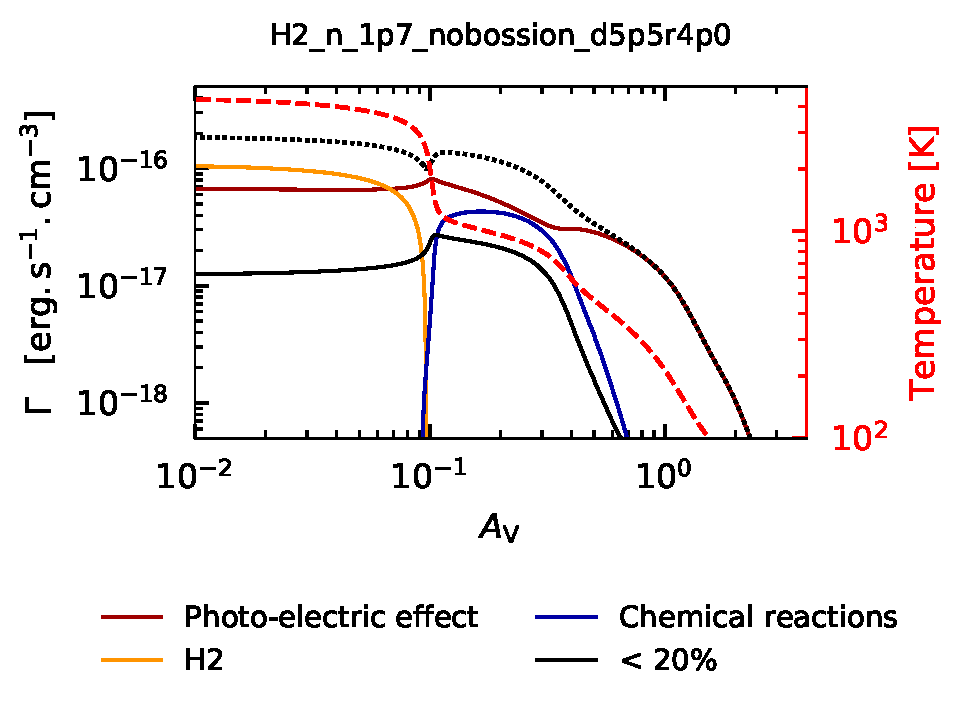
\includegraphics[trim = {0 0 0 1cm },clip,width=1\textwidth]{figure/H2/bosse_dcte_janevVSglover/glover/heat.pdf}
        \caption{Prescription de Glover}
    \end{subfigure}
    \caption{Profils des taux de chauffages d'un modèle à densité constante ($n_\mathrm{H} = 10^{5.5}$ et $\chi = 10^4$) utilisant la prescription de Janev ou de Glover. La température est représentée en tiret rouge. Le taux de chauffage total est en pointillé noir.}
    \label{fig:H2:bosse:heat}
\end{figure}


% \begin{figure}[!h]
%     \centering
%     \begin{subfigure}[t]{0.49\textwidth} % "0.49" donne ici la largeur de l'image
%         \centering 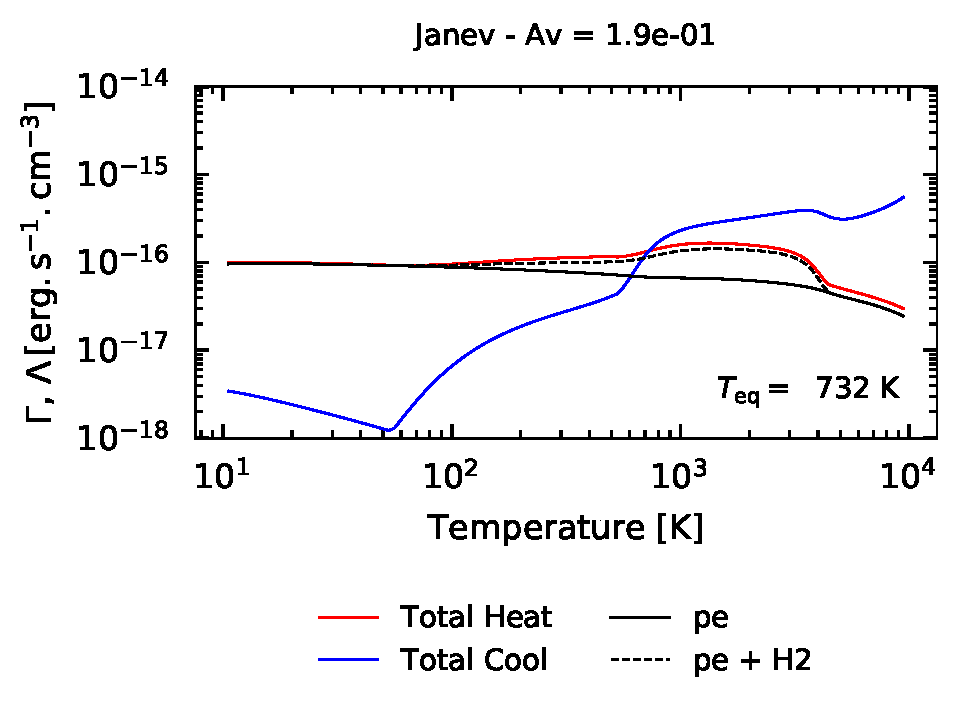
\includegraphics[trim = {0 0 0 1cm },clip,width=1\textwidth]{figure/H2/bosse_dcte_janevVSglover/janev/GC_h_1p9em01.pdf}
%         \caption{Prescription de Janev}
%     \end{subfigure}
%     \begin{subfigure}[t]{0.49\textwidth}
%         \centering 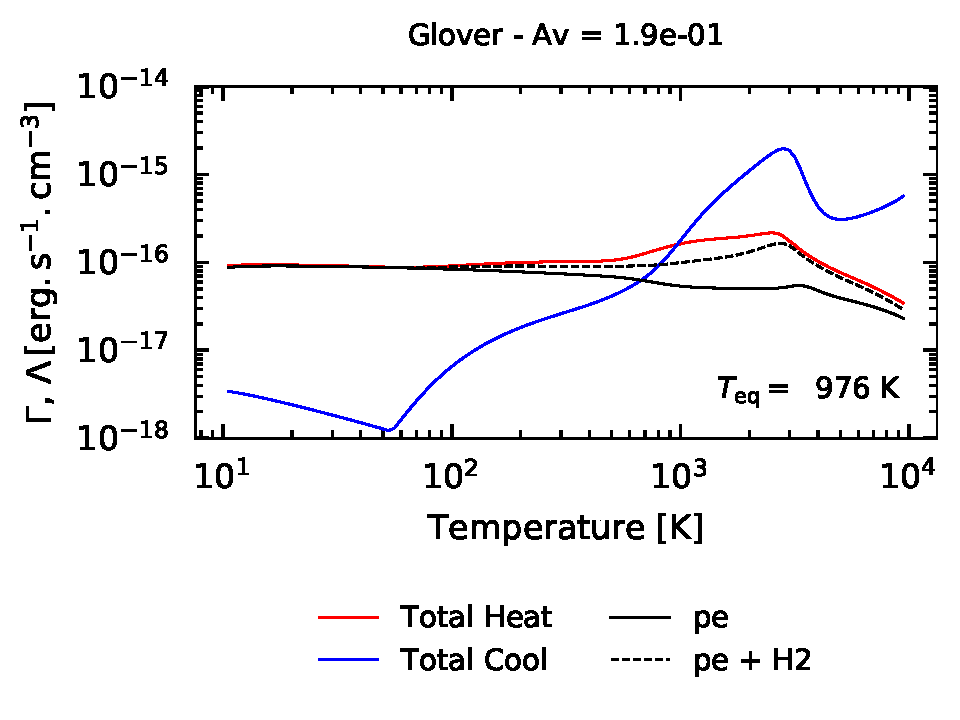
\includegraphics[trim = {0 0 0 1cm },clip,width=1\textwidth]{figure/H2/bosse_dcte_janevVSglover/glover/GC_h_1p9em01.pdf}
%         \caption{Prescription de Glover}
%     \end{subfigure}
%     ~
%     \begin{subfigure}[t]{0.49\textwidth} % "0.49" donne ici la largeur de l'image
%         \centering 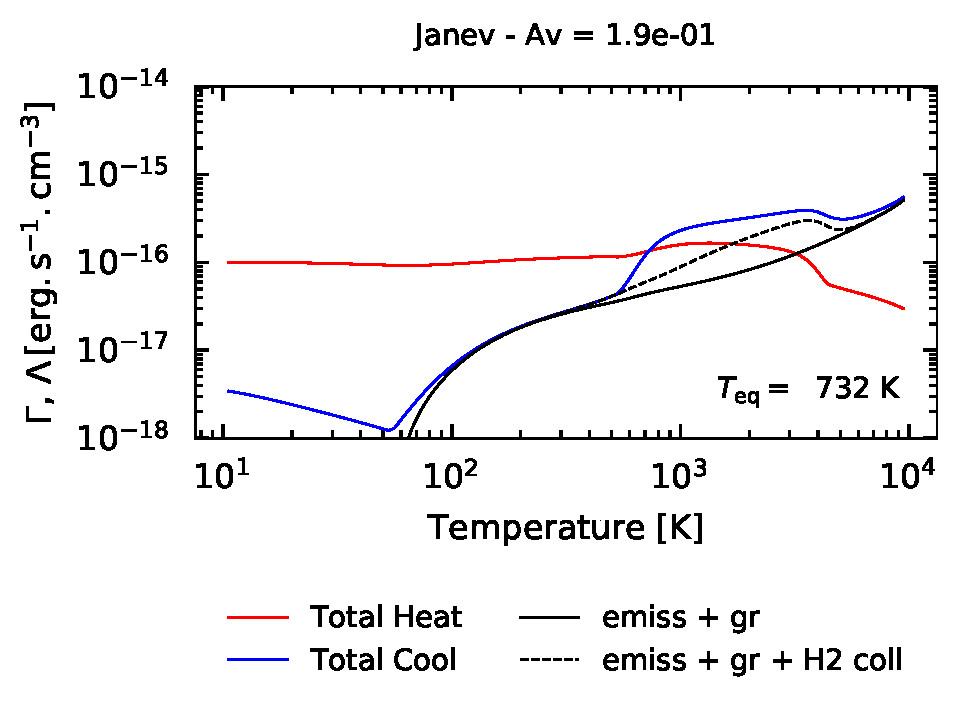
\includegraphics[trim = {0 0 0 1cm },clip,width=1\textwidth]{figure/H2/bosse_dcte_janevVSglover/janev/GC_c_1p9em01.pdf}
%         \caption{Prescription de Janev}
%     \end{subfigure}
%     \begin{subfigure}[t]{0.49\textwidth}
%         \centering 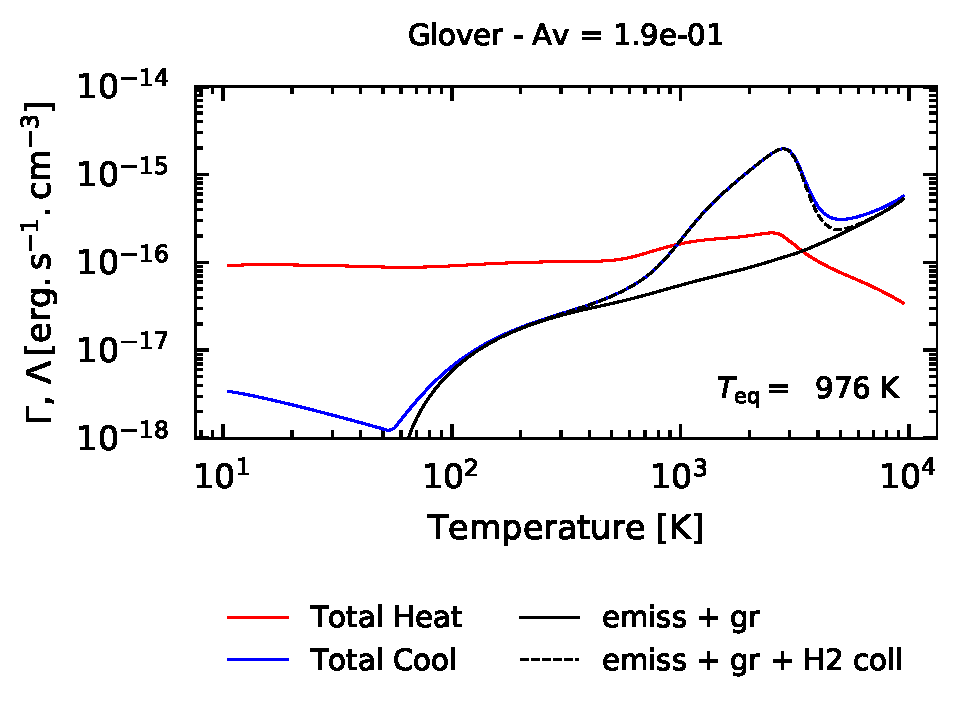
\includegraphics[trim = {0 0 0 1cm },clip,width=1\textwidth]{figure/H2/bosse_dcte_janevVSglover/glover/GC_c_1p9em01.pdf}
%         \caption{Prescription de Glover}
%     \end{subfigure}
%     \caption{Taux de chauffages et de refroidissements en fonction de la température à $A_\mathrm{v}$ de $0.2 \ \mathrm{mag}$ pour un modèle à densité constante ($n_\mathrm{H} = 10^{5.5}$ et $\chi = 10^4$).}
%     \label{fig:H2:bosse:GC}
% \end{figure}

\begin{figure}[!h]
    \centering
    \begin{subfigure}[t]{0.49\textwidth} % "0.49" donne ici la largeur de l'image
        \centering 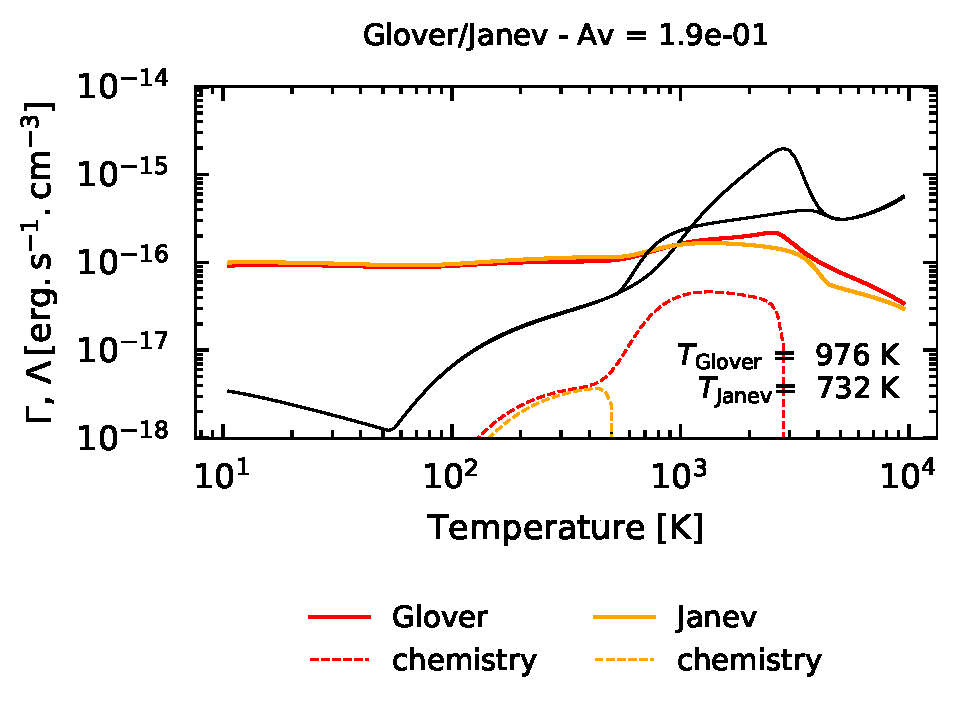
\includegraphics[trim = {0 0 0 1cm },clip,width=1\textwidth]{figure/H2/bosse_dcte_janevVSglover/GCcomp_h_1p9em01.pdf}
        \caption{Chauffage}
    \end{subfigure}
    \begin{subfigure}[t]{0.49\textwidth}
        \centering 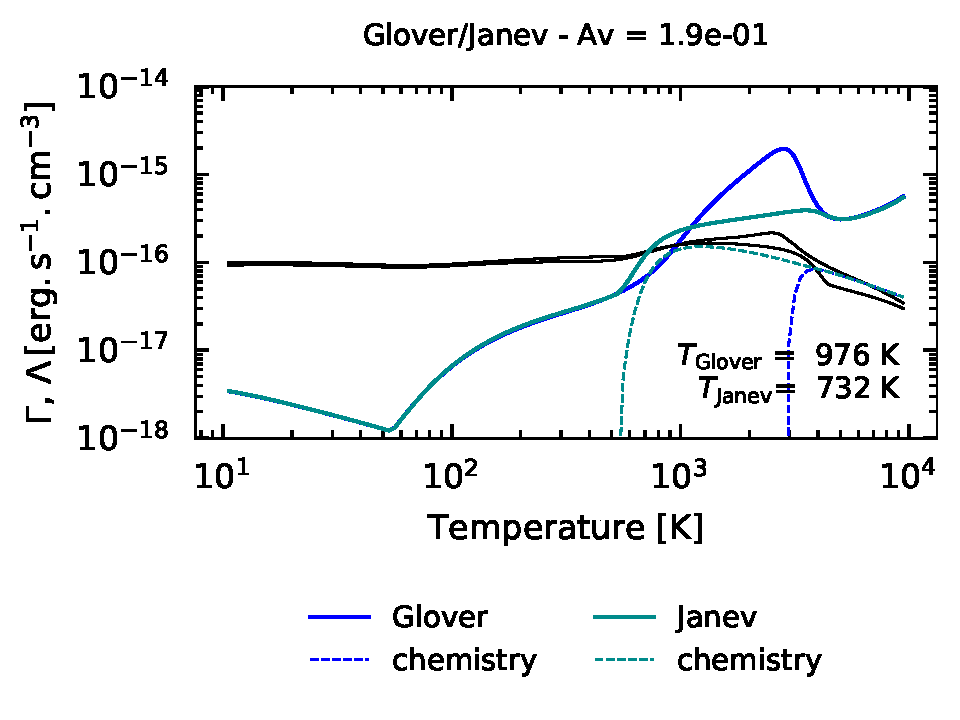
\includegraphics[trim = {0 0 0 1cm },clip,width=1\textwidth]{figure/H2/bosse_dcte_janevVSglover/GCcomp_c_1p9em01.pdf}
        \caption{Refroidissement}
    \end{subfigure}
    \caption{Efficacité du chauffage des réactions chimiques en fonction de la température pour un modèle à densité constante ($n_\mathrm{H} = 10^{5.5}$ et $\chi = 10^4$). Les courbes en rouge et jaune sur la figure (a) représente les processus de chauffage tandis que celles en noires les courbes de refroidissement total. Sur la figure (b), les courbes en bleu et bleu clair représentent le refroidissement alors que celles en noires le chauffage.}
    \label{fig:H2:bosse:chem}
\end{figure}

L'augmentation de température est provoquée par le changement d'allure de la courbe de refroidissement total ce qui déplace le point d'équilibre vers des températures plus chaudes. Les conséquences sont importantes. Plus de $\mathrm{CO}$ chaud parvient à se former après la transition $\mathrm{H}/\mathrm{H}_2$ donnant des raies (figure \ref{fig:H2:bosse:ICO}) plus intenses. Les raies $ 8 \leq \mathrm{J}\leq 15$ doublent leur intensités tandis que les raies $\mathrm{J}\geq 15$ augmente d'un facteur 10 ce qui est majeur. Elle permet notamment de retrouver des les diagrammes d'intensité du $\mathrm{CO}$ observée (\cite{COJoblin}). La figure \ref{fig:H2:bosse:IgridCO} trace les diagrammes d'intensités du $\mathrm{CO}$ pour une grille de modèle. Comme l'augmentation locale agit après la transition $\mathrm{H}/\mathrm{H}_2$ et que le $\mathrm{CO}$ est un traceur moléculaire, la figure \ref{fig:H2:bosse:IgridCO} montre l'impact global de l'augmentation de la température à la transition. Elle concerne les mêmes régions PDR que la figure \ref{fig:H2:JanevGlover:THH2}. 

\begin{figure}[!p]
    \centering
    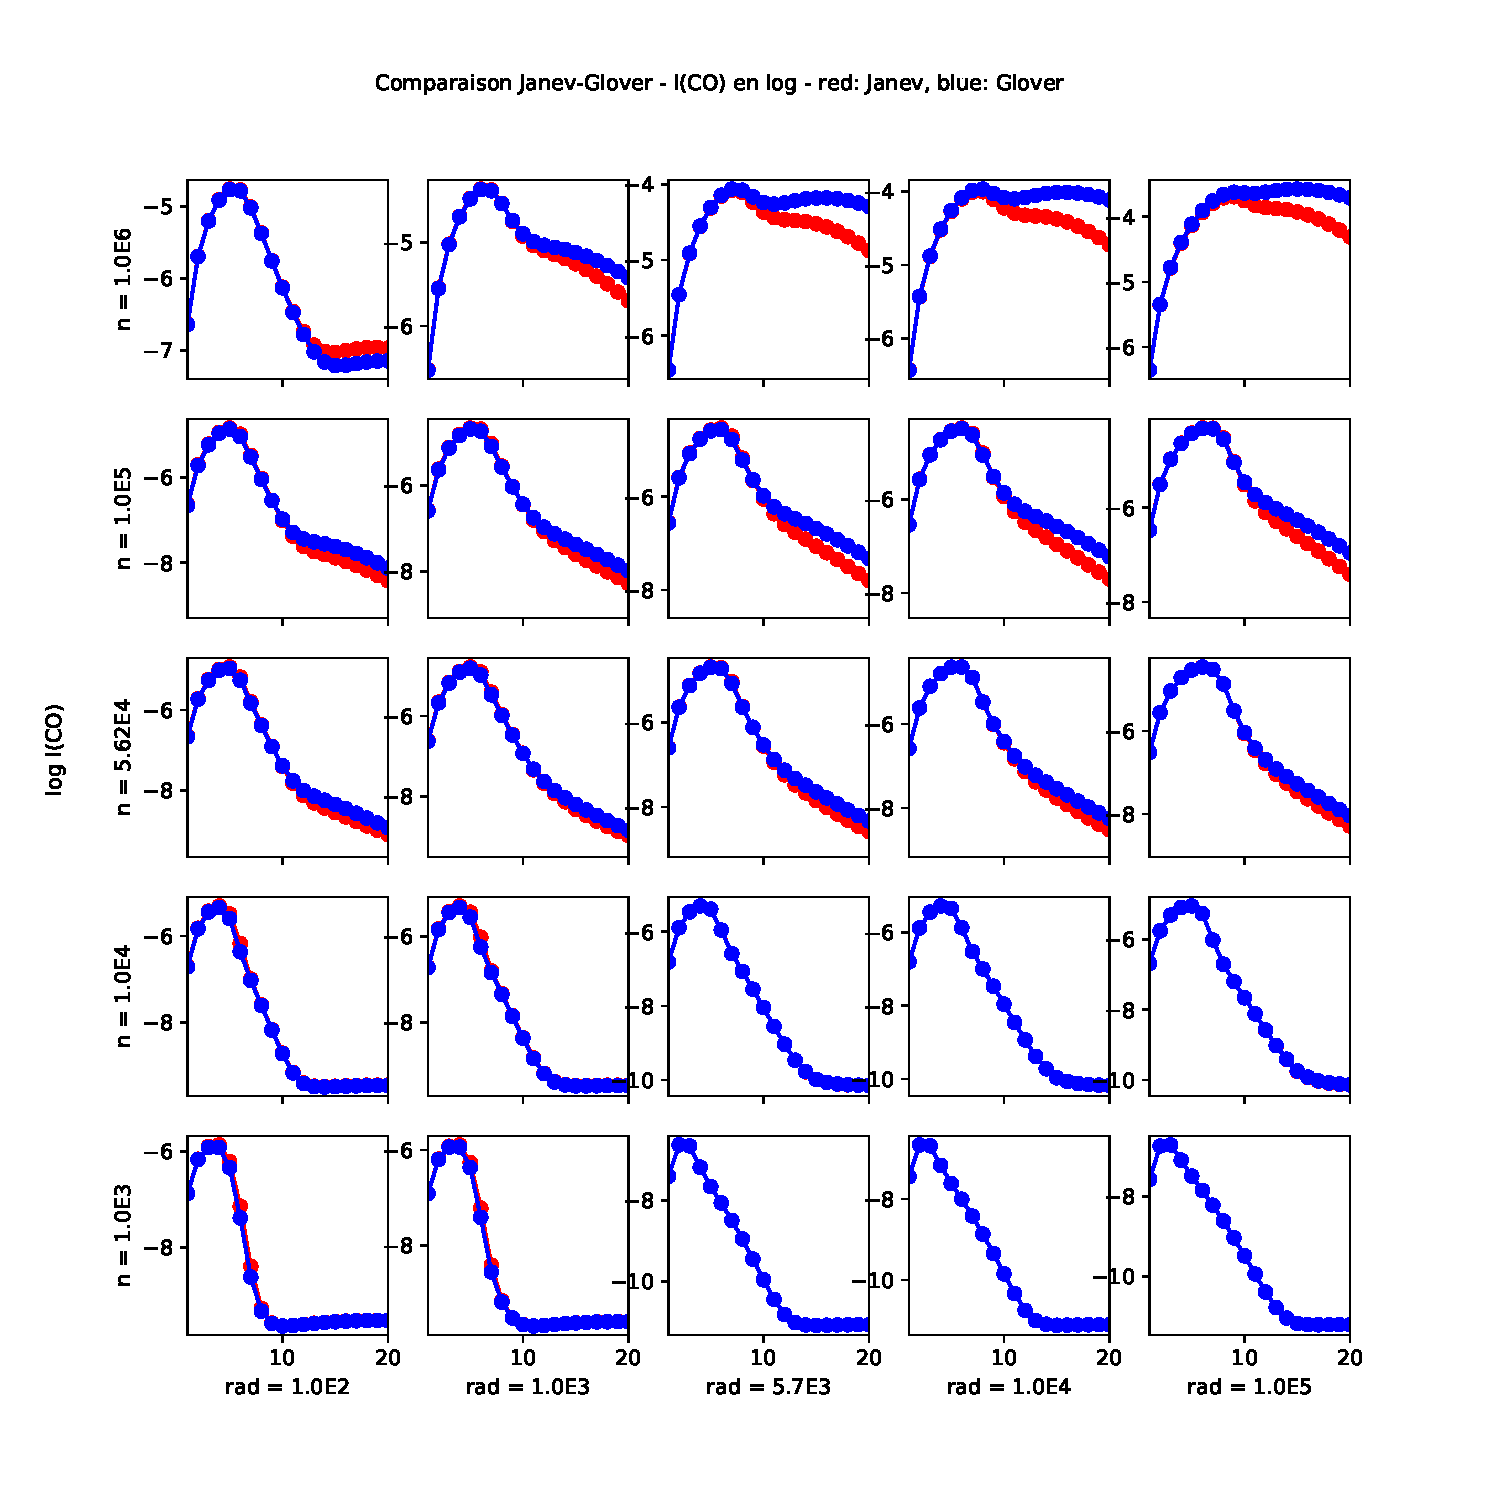
\includegraphics[trim = {0 0 0 3cm },clip,width=1\textwidth]{figure/H2/bosse_dcte_janevVSglover/PlotComp_Janev_Glover_IntCO.pdf}
    \caption{Diagramme d'intensité des raies du $\mathrm{CO}$ pour une grille de modèles à densité constante. Les lignes en rouge sont les modèles utilisant la prescription de Janev tandis que celles en bleues utilisent la prescription de Glover. Les $20$ premières transitions sont représentées.}
    \label{fig:H2:bosse:IgridCO}
\end{figure}



\subsection{Nouveaux taux de collisions de $\mathrm{H}_2$}

On a vu dans les sections précédentes qu'une nouvelle chimie du $\mathrm{H}_2$ pouvait avoir un impact fort sur les profils de densité et de température du gaz. Nous cherchons maintenant à affiner la physique qui décrit le phénomène de chauffage par $\mathrm{H}_2$. Afin de calculer le taux de chauffage par desexcitation collisionnelle, le code PDR effectue le bilan des transitions collisionnelles des niveaux de $\mathrm{H}_2$. Il dépend directement des taux de collision $k_{ij}$ qui donnent la probabilité d'une transition de l'état $i$ à l'état $j$ par collision avec une espèce du gaz. On connaissait ces $k_{ij}$ seulement pour les états peu énergétiques du $\mathrm{H}_2$ ($J\leq15$ de l'état fondamentale). De récents calculs de chimie semi-classique ont permis d'estimer avec précision les taux de collisions jusqu'à des niveaux très énergétiques \cite{Bossion}. \newline 


Une étude rapide a montré que l'utilisation des nouveaux taux de collisions montrait que $H_2$ chauffait globalement les bords atomiques de $+100$K (figure \ref{fig:H2:Bossion:Tba}). On sait que $\mathrm{H}_2$ peut provoquer une instabilité thermique, dans différentes zones du nuage, mais pour des conditions physiques que que l'on ne connait pas. Le code PDR obtient des températures en bords atomique de nuage plus chaude pour les PDR denses et peu illuminées, avec les nouveaux taux de collisions ce qui suggère l'existence d'une instabilité thermique. En effet, le code PDR ne pouvant déterminer qu'une température d'équilibre, des PDR qui était anciennement à la température d'équilibre froide deviennent chaude provoquant un $\Delta T$ important. \newline 
En revanche, la comparaison des températures maximales atteintes par les PDR peuvent montrer de nouvelles régions de l'espace des paramètres impactées par l'utilisation des nouveaux taux de collisions (figure \ref{fig:H2:Bossion:Tmax}). Les bords atomiques des PDR étant les zones les plus proche de la source de photons, elles sont généralement les plus chaudes à travers le nuage. La carte \ref{fig:H2:Bossion:Tmax} doit, à priori, englober la carte de température du bord atomique des PDR. Pourtant, ce n'est pas le cas dans certaines conditions physiques de PDR. 

\begin{figure}[!h]
    \centering
    \begin{subfigure}[t]{0.49\textwidth} % "0.49" donne ici la largeur de l'image
        \centering 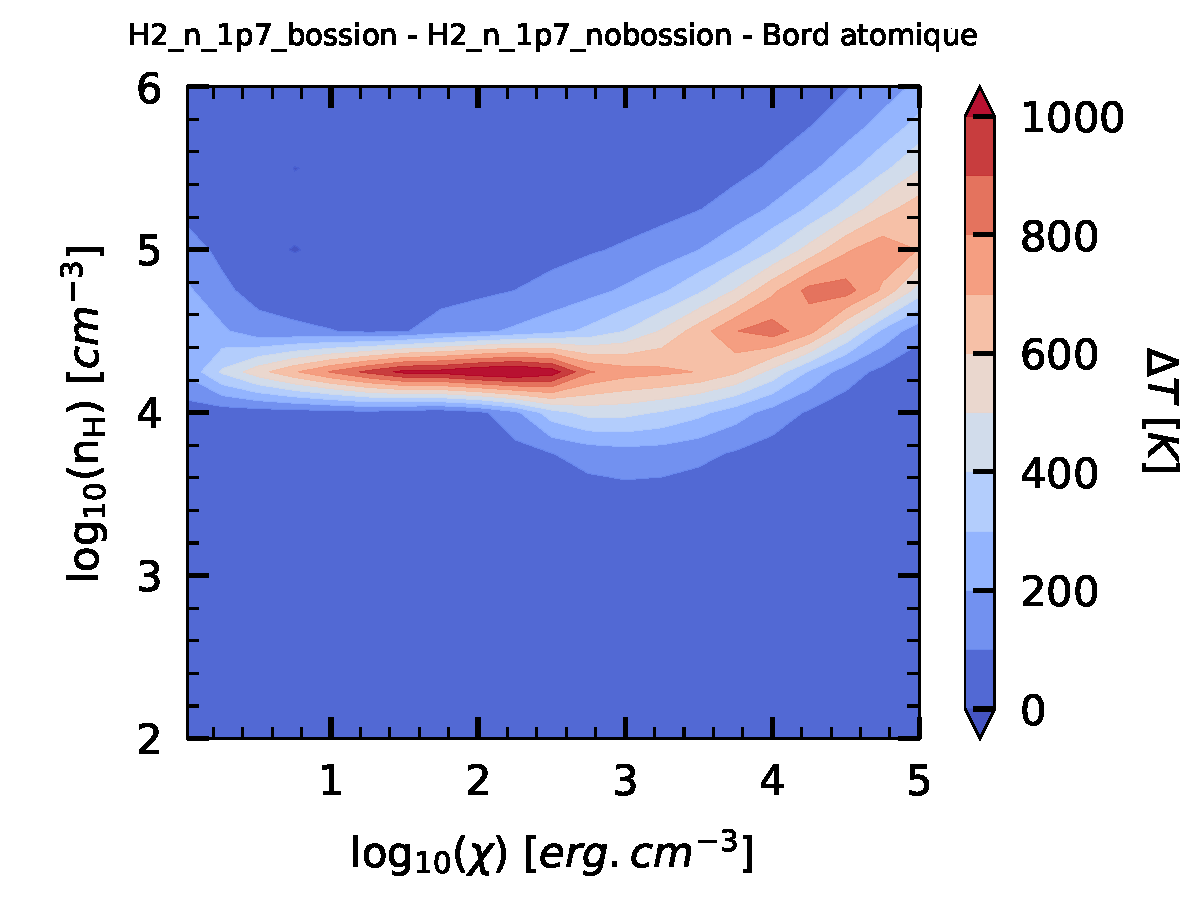
\includegraphics[trim = {0 0 0 1cm },clip,width=1\textwidth]{figure/H2/diffgrid_bossionglover/mapTba_H2_n_1p7_bossion_H2_n_1p7_nobossion.pdf}
        \caption{Différence de température au bord}
        \label{fig:H2:Bossion:Tba}
    \end{subfigure}
    ~ 
    \begin{subfigure}[t]{0.49\textwidth}
        \centering 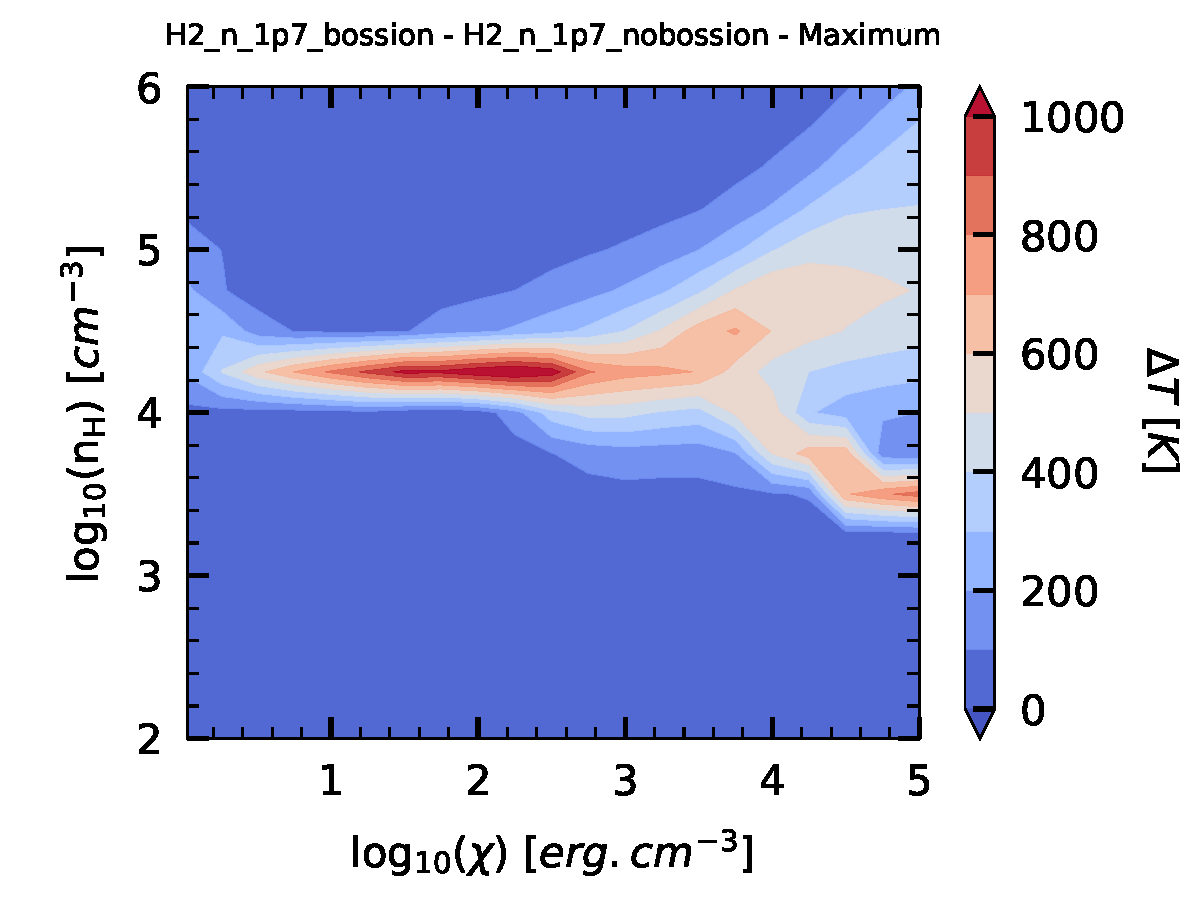
\includegraphics[trim = {0 0 0 1cm },clip,width=1\textwidth]{figure/H2/diffgrid_bossionglover/mapTmax_H2_n_1p7_bossion_H2_n_1p7_nobossion.pdf}
        \caption{Différence de température maximale}
         \label{fig:H2:Bossion:Tmax}
    \end{subfigure}
    \caption{Carte de température comparant l'impact des nouveaux taux de collisions de $\mathrm{H}_2$ sur des modèles à densités constantes.}
\end{figure}


\subsubsection{Etude des courbes de chauffage et de refroidissement}


En traçant les profils de densités d'un modèle ($n_\mathrm{H} = 10^{3.5}\,\mathrm{cm}^{-3},\chi = 10^{4.5}$) on constate une augmentation brutale de la température à la fin de la zone atomique vers $A_\mathrm{v}=0.7\,\mathrm{mag}$ (figure \ref{fig:H2:Bossion:profilT}) accompagné d'une diminution de la densité de $\mathrm{H}_2$. Les courbes de chauffage et de refroidissement (figure \ref{fig:H2:Bossion:zer}) à cet endroit du nuage montre qu'il existe une bistabilité thermique provoquée par un emballement de l'effet photoélectrique à partir de $T\geq800$K et du refroidissement par $\mathrm{H}_2$. Elle existait déjà sans les nouveaux taux de collisions et diminue même l'emballement de l'effet photoélectrique. Les figures \ref{fig:H2:Glover:cooling} et \ref{fig:H2:Bossion:cooling} montrent séparément les courbes de chauffage et de refroidissement pour les deux modèles utilisant ou non les nouveaux taux. De plus, elles pointent une ambiguïté dans les fichiers \textit{.res} sur le calcul des totaux notamment sur les termes de refroidissement. En effet, la somme des colonnes de refroidissement dépasse celle du total donnée par le code. Comme j'ai préféré me fier aux processus plutôt qu'au total, les courbes de total on était recalculée à partir des autres colonnes. Cela amène à la situation où l'on ne parvient pas toujours à retrouver la température prédite par le code avec celle donnée par l'intersection des courbes de chauffage et de refroidissement (figure \ref{fig:H2:Bossion:cooling}). Je n'ai pas eu le temps de chercher les raisons de cette différence. Deux autres points remarquables : à basse température ($T\geq 100$K) le refroidissement total devient négatif à cause des termes de refroidissement par les raies de $\mathrm{C}^+$ et de $\mathrm{O}$ mais aussi par le couplage gaz-grains qui devient chauffant ; la colonne \textit{refrec} qui est le refroidissement par recombinaison électroniques des ions est comptabilisé comme un terme négatif alors que les autres colonnes de refroidissement sont positives. \newline


\begin{figure}[!h]
    \centering
    \begin{subfigure}[t]{0.49\textwidth} % "0.49" donne ici la largeur de l'image
        \centering 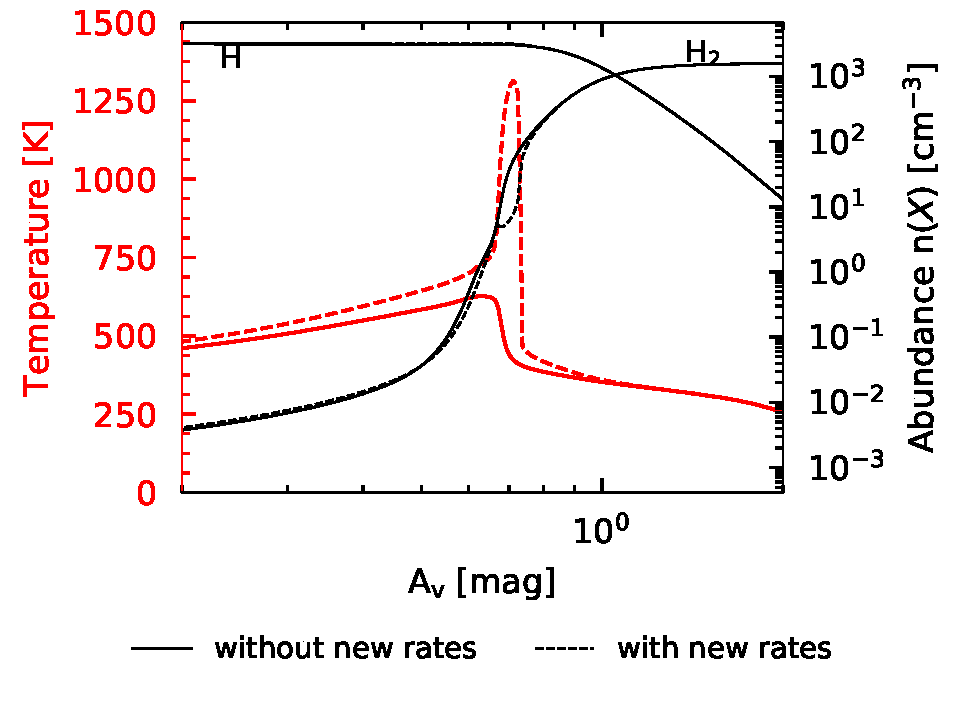
\includegraphics[trim = {0 0 0 0cm },clip,width=1\textwidth]{figure/H2/pic/profilT.pdf}
        \caption{Profils de densité et température}
        \label{fig:H2:Bossion:profilT}
    \end{subfigure}
    ~ 
    \begin{subfigure}[t]{0.49\textwidth}
        \centering 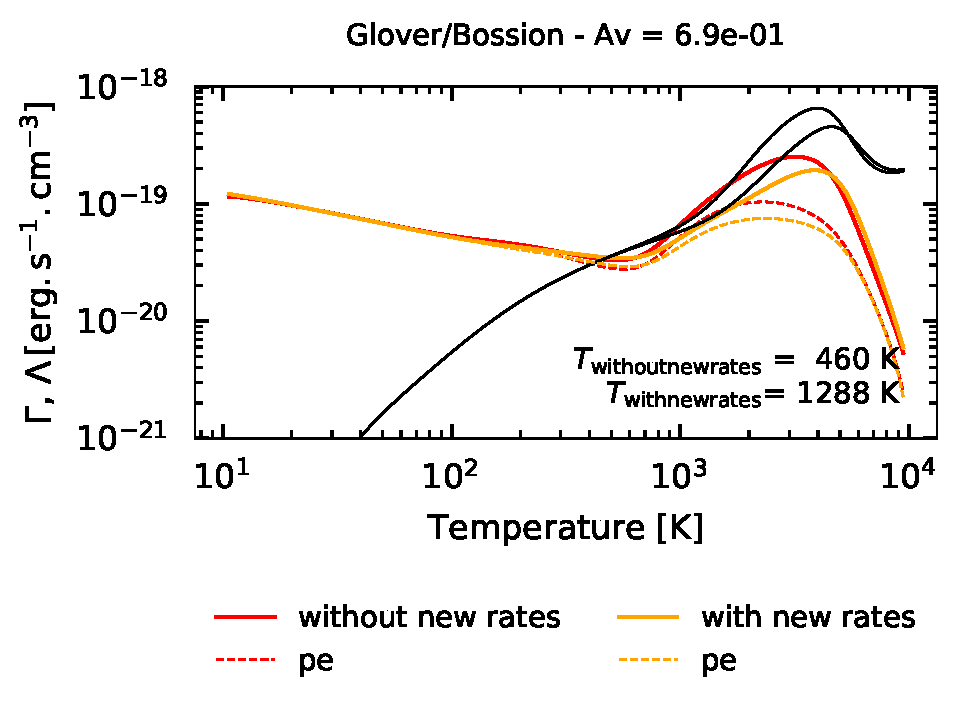
\includegraphics[trim = {0 0 0 1cm },clip,width=1\textwidth]{figure/H2/pic/GCcomp_h_6p9em01.pdf}
        \caption{Courbes de chauffages à $A_\mathrm{v}=0.7\,\mathrm{mag}$}
         \label{fig:H2:Bossion:zer}
    \end{subfigure}
    \caption{Modèle à densité constante ($n_\mathrm{H} = 10^{3.5}\,\mathrm{cm}^{-3}$ et $\chi = 10^4$).}
    \begin{minipage}{\textwidth}
    Sur (b), les courbes de chauffage total sont représentées en trait plein rouge et orange. Les traits noirs sont les courbes de refroidissement total qui est principalement assuré par les émissions de $\mathrm{C}^+$ et de $\mathrm{O}$, le couplage gaz-grains et le refroidissement par les émissions ro-vibrationnelle du $\mathrm{H}_2$ particulièrement actif entre $T\sim10^3-10^4$K.
    \end{minipage}
\end{figure}

\begin{figure}[!h]
    \centering
    \begin{subfigure}[t]{0.49\textwidth} % "0.49" donne ici la largeur de l'image
        \centering 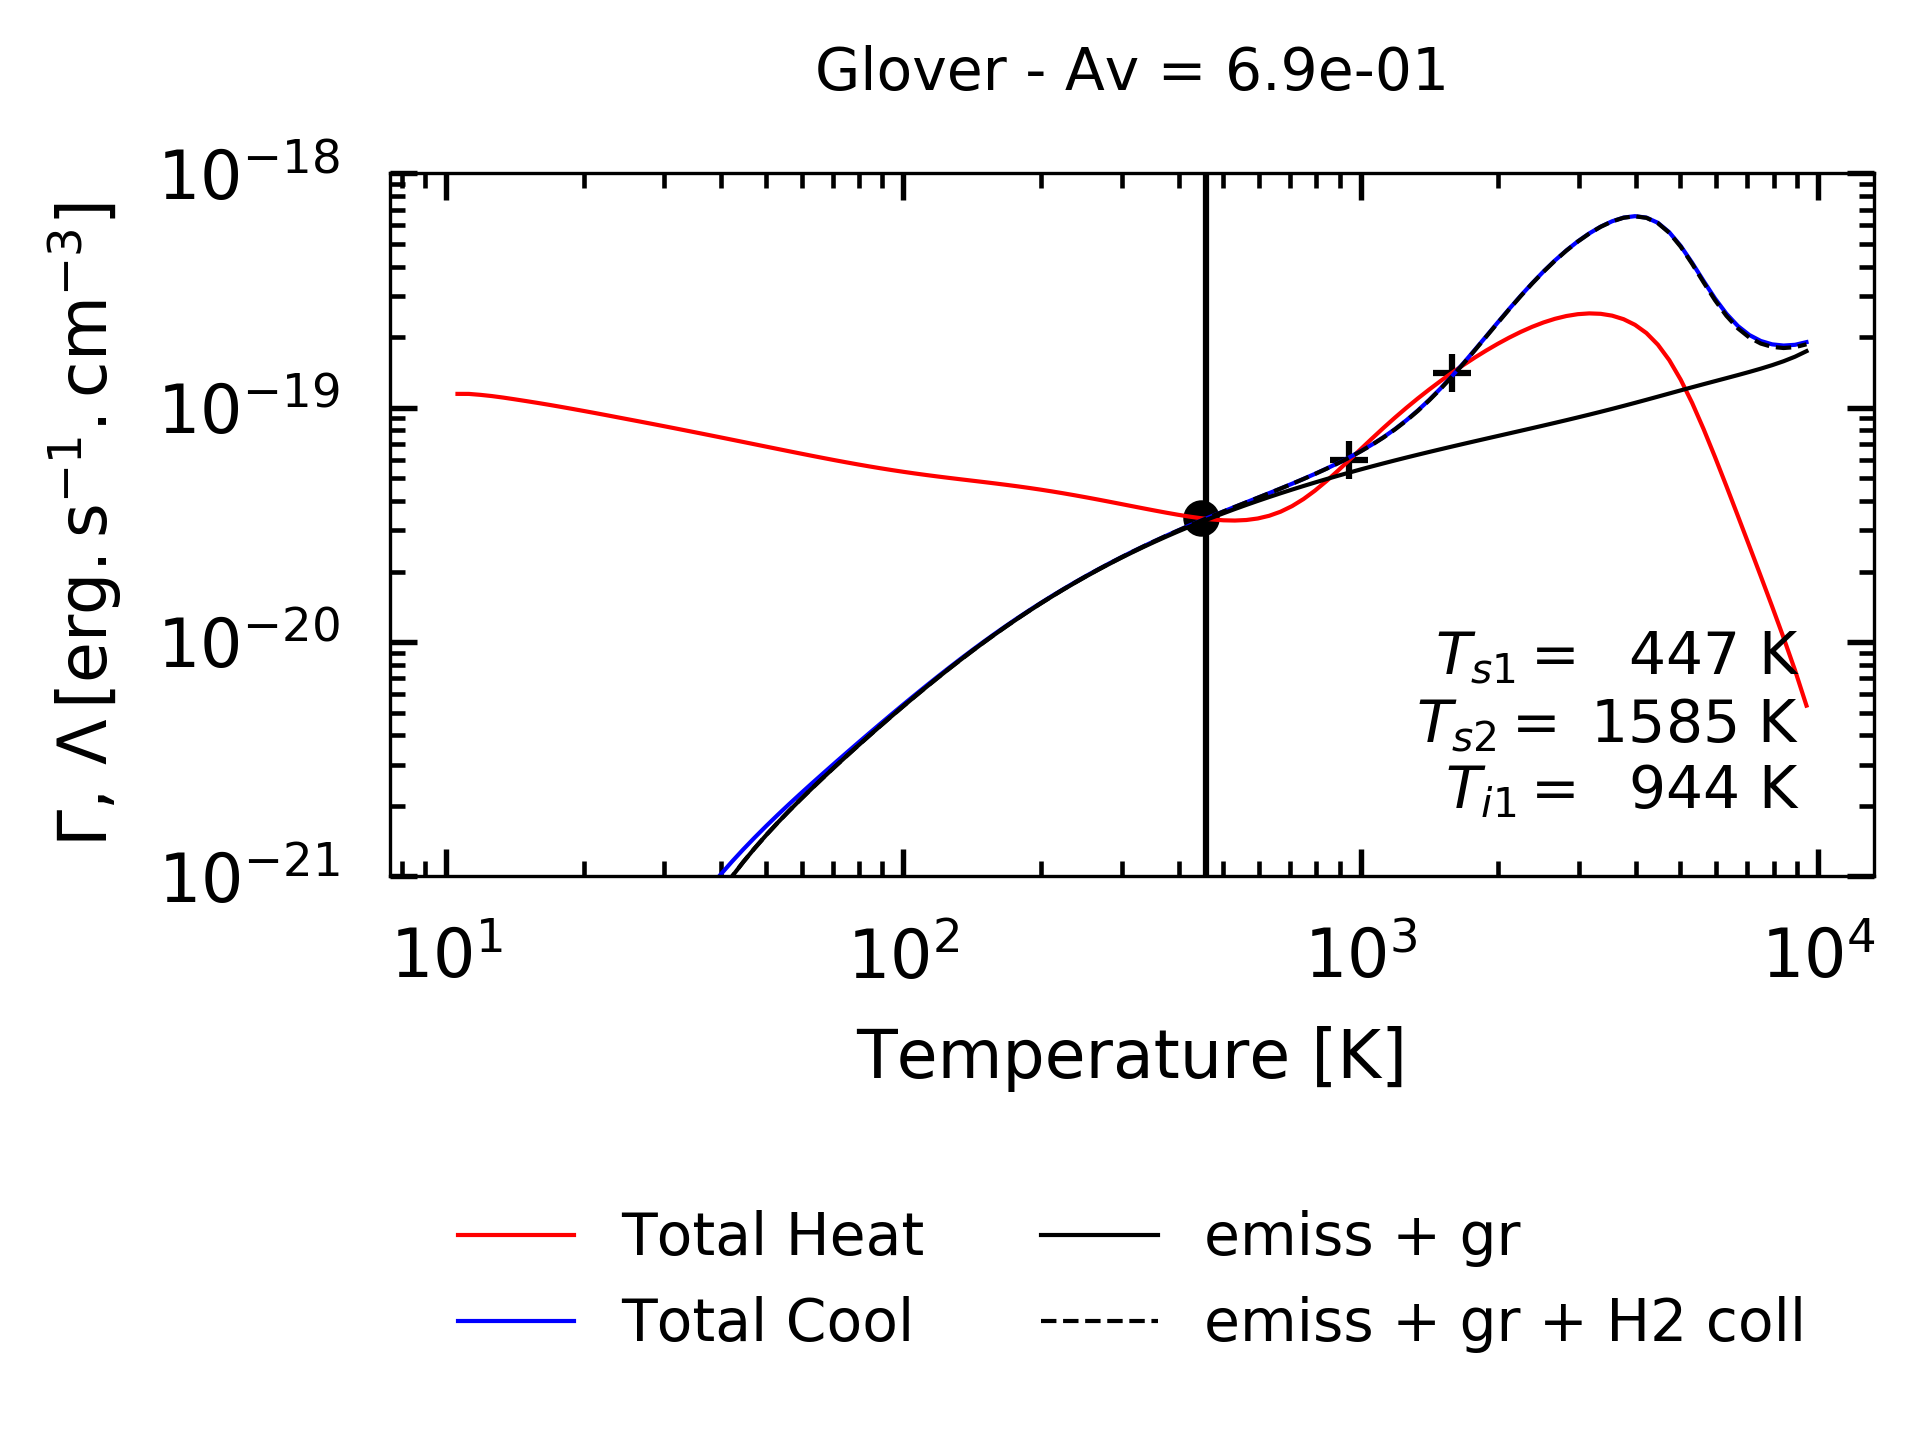
\includegraphics[trim = {0 0 0 1cm },clip,width=1\textwidth]{figure/H2/pic/glover_cooling.png}
        \caption{Sans les nouveaux taux}
        \label{fig:H2:Glover:cooling}
    \end{subfigure}
    ~ 
    \begin{subfigure}[t]{0.49\textwidth}
        \centering 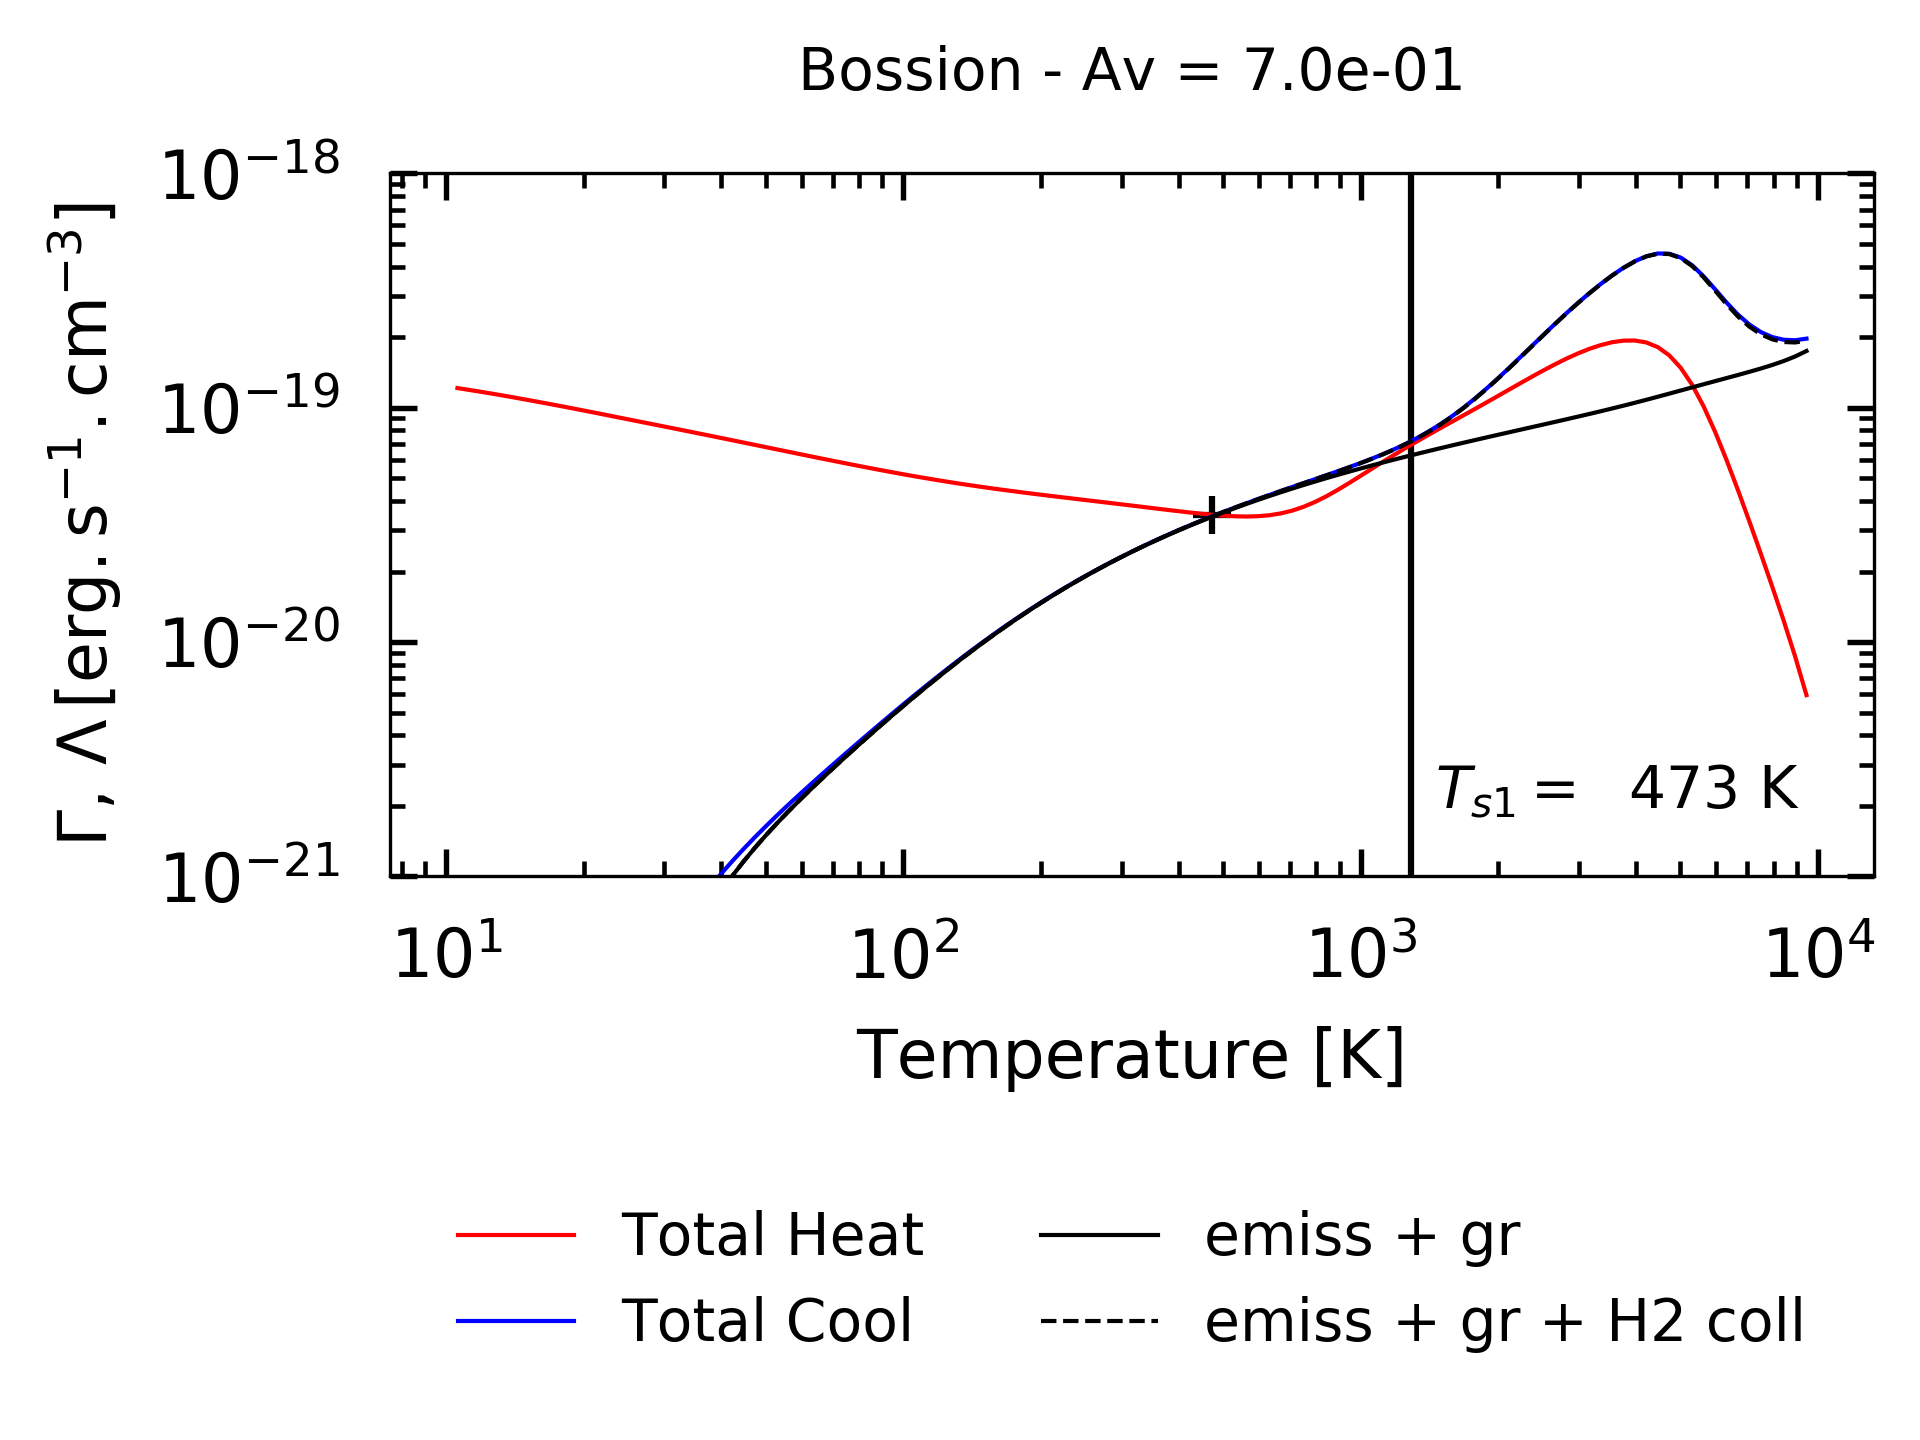
\includegraphics[trim = {0 0 0 1cm },clip,width=1\textwidth]{figure/H2/pic/bossion_cooling.png}
        \caption{Avec les nouveaux taux}
         \label{fig:H2:Bossion:cooling}
    \end{subfigure}
    \caption{Courbes de chauffage et de refroidissement à $A_\mathrm{v}=0.7\,\mathrm{mag}$}
    \begin{minipage}{\textwidth}
    Les traits verticaux représentent la température d'équilibre trouvé par le code PDR. Les marqueurs (cercle plein et croix vertical) sont calculées comme les intersections des courbes de chauffage et de refroidissement. La température d'équilibre choisie par le code est indiqué par le cercle plein tandis que les autres solutions trouvées sont indiquée par une croix vertical.
    \end{minipage}
\end{figure}


\subsection{Amplification de l'effet photoélectrique par le carbone}

J'ai analysé la chimie du nuage à $A_\mathrm{v} = 0.7\,\mathrm{mag}$ et compris que l'amplification de l'effet photoélectrique fonctionnait selon un mécanisme similaire à celui induit par le chlore. Ici l'atome de chlore est remplacé par l'atome de carbone et la recombinaison des ions chlore par transfert de charge par la formation par $\mathrm{H}_2$ suivie de la dissociation radiative de la molécule $\mathrm{CH}^+$. Un schéma, certes peu ragoûtant mais somme toute explicatif, résume le mécanisme de chauffage (figure \ref{fig:H2:meca:C}). Le carbone ayant un potentiel de ionisation de $11.3\,\mathrm{eV}$ il peut être photoionisé. La présence d'une grande quantité de $\mathrm{H}_2$ excité à cette position du nuage permet la formation du $\mathrm{CH}^+$ qui se dissocie radiativement formant un ion $\mathrm{H}^+$ et un atome $\mathrm{C}$ qui peut de nouveau être photoioniser. Comme pour le chlore, ce mécanisme permet de former efficacement une grande quantité d'électrons qui emballe l'effet photoélectrique sur les grains. J'ai identifié les réactions principales en jeu et construit un modèle permettant de retrouver l'augmentation de la fraction électronique à haute température.

\begin{figure}[!h]
    \centering 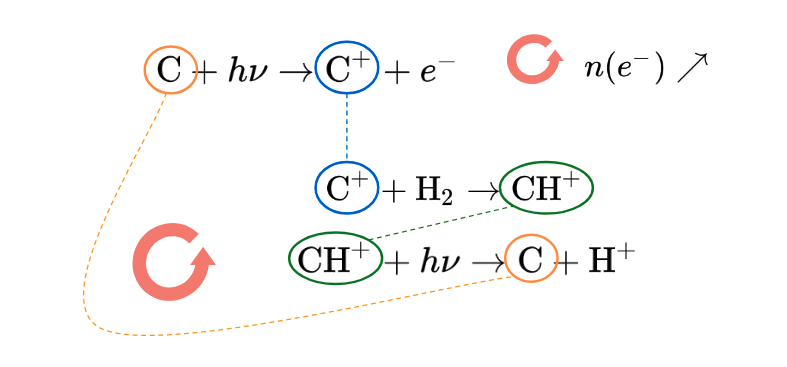
\includegraphics[trim = {0 0 0 1cm},clip,width=0.6\textwidth]{figure/H2/pic/scheme_pic.png}
    \caption{Mécanisme de l'instabilité induit par le carbone}
    \label{fig:H2:meca:C}
\end{figure}


\subsubsection{ion hydrogène}

Les réactions efficaces qui concernent les ions hydrogènes dans cette région du nuage sont : 

\begin{equation}\label{eq:sysH}
    \begin{array}{lllllllr}
        \mathrm{D}^+ & + &\mathrm{H}   & \rightleftharpoons &\mathrm{D}  & + & \mathrm{H}^+ &   \\
        \mathrm{O}^+ & + &\mathrm{H}   & \rightleftharpoons &\mathrm{O}  & + & \mathrm{H}^+ &   \\
        \mathrm{H}^+  & + & \mathrm{e}^-  & \rightarrow &\mathrm{H}   &   &  &  \\
        \mathrm{H}^+  & + & \mathrm{grains}  & \rightarrow &\mathrm{H}   &   &  &  \\
        \mathrm{CH}^+ & + & h\nu   & \rightarrow &\mathrm{C}  & + & \mathrm{H}^+ &  \\
    \end{array}
\end{equation}

On ne prend pas en compte les réactions impliquant $\mathrm{D}$ et $\mathrm{O}$ car elles forment autant de $\mathrm{H}^+$ qu'elles détruisent. On néglige dans un premier temps la recombinaison de $\mathrm{H}^+$ sur les grains qui ne modifie que très peu le profil de densité de l'ion en fonction de la température. Il reste :

\begin{equation}
    \begin{array}{lllllllr}
        \mathrm{CH}^+ & + & h\nu   & \rightarrow &\mathrm{C}  & + & \mathrm{H}^+ & (\mathcal{P}_{ch}) \\
        \mathrm{Cl}  & + & \mathrm{H}^+  & \rightarrow & \mathrm{Cl}^+ & + &\mathrm{H}  & (\mathcal{B}_h) \\
    \end{array}
\end{equation}
avec $\mathcal{P}_{ch}$ en $\mathrm{s}^{-1}$ et $\mathcal{B}_h$ en $\mathrm{cm}^{-3}\mathrm{s}^{-1}$ les coefficients de réactions.

Le bilan de formation donne : 

\begin{equation}
    \frac{d}{dt}n(\mathrm{H}^+) = \mathcal{P}_{ch}n(\mathrm{CH}^+) - \mathcal{B}_{h}n(\mathrm{H}^+)n(e^-)
\end{equation}

ce qui donne en considérant que $n(e^-)\approx n(\mathrm{H}^+)$ : 

\begin{equation}
\boxed{
    n(\mathrm{H}^+) = \sqrt{\frac{\mathcal{P}_{ch}}{\mathcal{B}_h}n(\mathrm{CH}^+)}
    }
\end{equation}

\subsubsection{molécule $\mathrm{CH}^+$}

De même les réactions impliquant la molécule $\mathrm{CH}^+$ sont :

\begin{equation}\label{eq:sysH}
    \begin{array}{lllllllr}
        \mathrm{C}^+ & + &\mathrm{H}_2   & \rightleftharpoons &\mathrm{CH}^+  & + & \mathrm{H} &   \\
        \mathrm{CH}^+  & + & \mathrm{e}^-  & \rightarrow &\mathrm{H}   & +  & \mathrm{C} &  \\
        \mathrm{CH}^+  & + & h\nu  & \rightarrow &\mathrm{C}^+   & +  & \mathrm{H} &  \\
    \end{array}
\end{equation}

On négligera seulement la recombinaison dissociation. On pose deux nouveaux coefficients de réactions $k_1$ et $k_2$ en $\mathrm{cm}^{-3}\mathrm{s}^{-1}$.

\begin{equation}
    \begin{array}{lllllllr}
    \mathrm{C}^+ & + & \mathrm{H}_2   & \rightarrow &\mathrm{CH}^+  & + & \mathrm{H} & (k_1) \\
    \mathrm{CH}^+ & + & \mathrm{H}   & \rightarrow &\mathrm{C}^+  & + & \mathrm{H}_2 & (k_2) \\
        \mathrm{CH}^+ & + & h\nu   & \rightarrow &\mathrm{C}  & + & \mathrm{H}^+ & (\mathcal{P}_{ch}) \\
    \end{array}
\end{equation}

Le bilan de formation du $\mathrm{CH}^+$ donne 

\begin{equation}
    \frac{d}{dt}n(\mathrm{CH}^+) = k_1 n(\mathrm{C}^+)n(\mathrm{H}_2) - k_2n(\mathrm{CH}^+)n(\mathrm{H}) -\mathcal{P}_{ch}n(\mathrm{CH}^+) 
\end{equation}

Même à $A_\mathrm{V} = 0.7 \,\mathrm{mag}$, l'hydrogène reste principalement atomique (voir figure \ref{fig:H2:Bossion:profilT}) et on a $n_\mathrm{H}\approx n(\mathrm{H})$. Il est également correct de poser $n(\mathrm{C}^+)\approx \delta_C n_\mathrm{H}$ dans la mesure où le carbone est principalement atomique. On obtient alors :

\begin{equation}
\boxed{
    n(\mathrm{CH}^+) = \frac{k_1\delta_Cn_\mathrm{H}}{\mathcal{P}_{ch} + k_2n_\mathrm{H}} n(\mathrm{H}_2)
    }
\end{equation}

Il faudrait maintenant chercher à estimer la densité de $\mathrm{H}_2$ en fonction de la température à cette position du nuage. 

\subsubsection{molécule $\mathrm{H}_2$}

Les réactions les plus efficaces sont  

\begin{equation}\label{eq:sysH}
    \begin{array}{lllllllr}
        \mathrm{H}    & + &\mathrm{H}::   & \rightarrow &\mathrm{H}_2  & & &   \\
        \mathrm{H}_2  & + & h\nu  & \rightarrow &\mathrm{H}   & +  & \mathrm{H} &  \\
        \mathrm{H}_2  & + & \mathrm{C}^+  & \rightarrow &\mathrm{H}   & +  & \mathrm{CH}^+ &  \\
    \end{array}
\end{equation}

Il est néanmoins difficile d'estimer le taux de formation de $\mathrm{H}_2$ sur les grains. En prenant les formules proposées dans \cite{Rollig2005} que j'ai fitté avec les taux de réactions données par le code, je n'ai pas pu obtenir des taux de formation et de destruction du $\mathrm{H}_2$ satisfaisant. J'ai donc choisi de ne pas chercher à estimer par la densité du $\mathrm{H}_2$ et ai pris celle donnée par le \textit{.res} pour le besoin de la démonstration.

\subsubsection{thermique}

Nous sommes maintenant en mesure d'estimer la densité d'électrons en fonction de la température. Le modèle que nous avons construit retrouve l'emballement de l'effet photoélectrique à partir de $T\geq 800$K ce qui prouve que nous avons compris le mécanisme de chauffage. On a calculé le refroidissement par les émissions de $\mathrm{H}_2$ (pointillé bleue) à partir d'une expression analytique (\cite{Rollig2005}, équation C.1) qui ne prend pas en compte que les états vibrationnelles. Or les émissions depuis les états rotationnels sont très efficaces pour refroidir le gaz c'est pourquoi on ne parvient pas à retrouver le refroidissement calculé par le code. 

\begin{figure}[!h]
    \centering 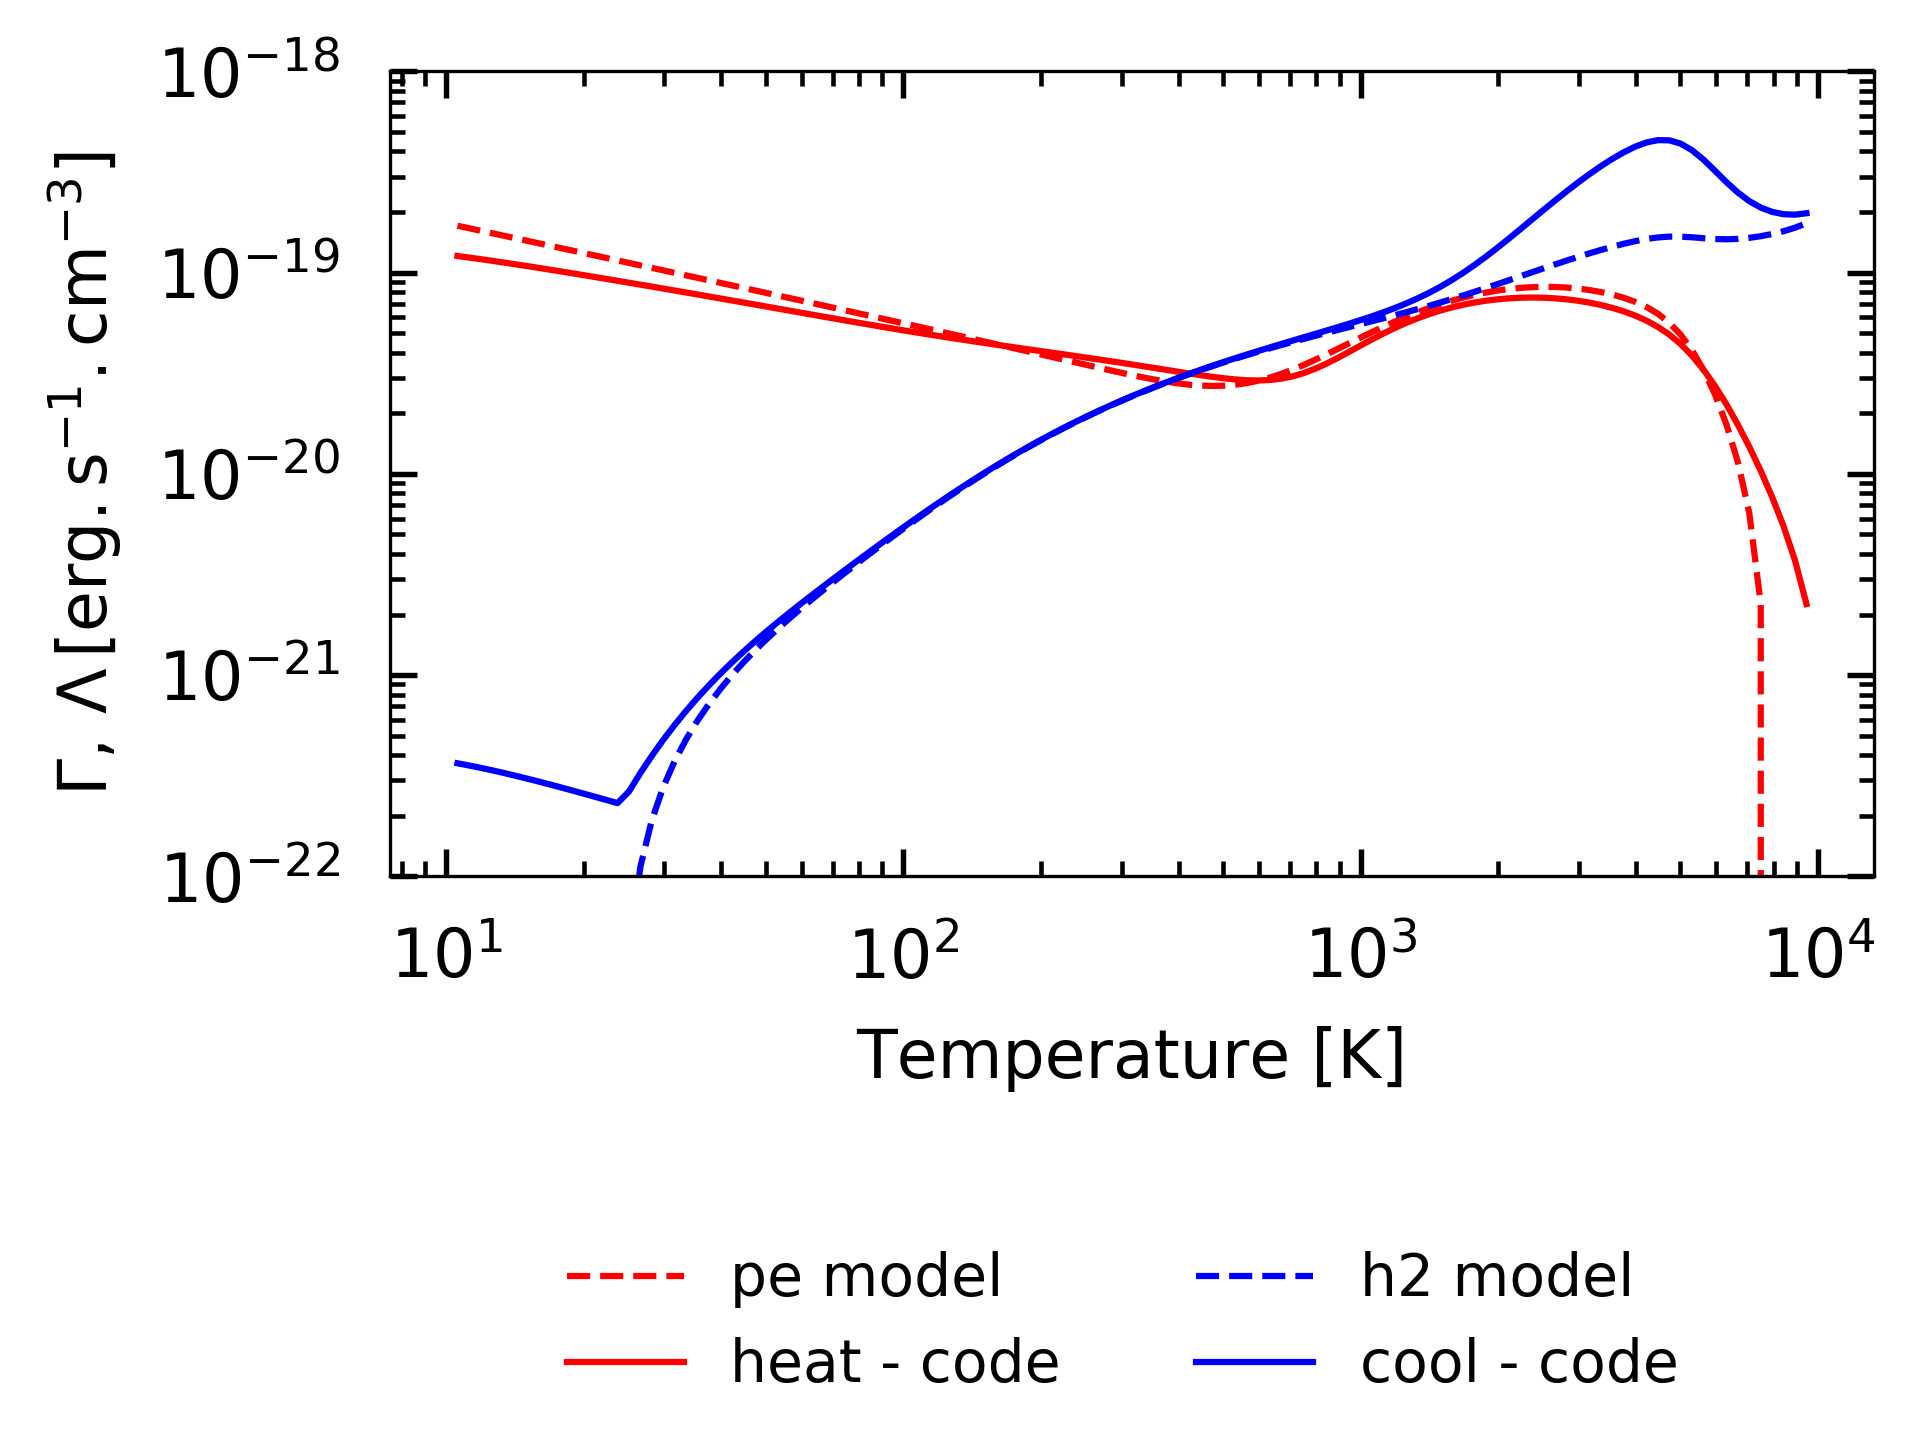
\includegraphics[trim = {0 0 0 0cm},clip,width=0.6\textwidth]{figure/H2/pic/model.png}
    \caption{Comparaison du modèle chimique avec le code PDR}
    \label{fig:H2:meca:chim}
\end{figure}


% \subsubsection{Raies du $\mathrm{CO}$ et $\mathrm{H}_2$ - Janev/Glover}
% à tracer en plus des profils de températures de modèles ...

% et on remarque plusieurs choses. Tout d'abord les raies d'émissions de $\mathrm{H}_2$ et $\mathrm{CO}$ sont augmentées (\autoref{figu:H2:..}). De plus le profil de température avec la nouvelle prescription (Glover) est modifié un tout petit peu au au bord (+100K) et un peu à l'entrée du nuage moléculaire (+400K) (\autoref{fig:H2:JanevGlover:emiss}). L'augmentation de la température à l'entrée du nuage moléculaire ($A_\mathrm{V} = 0.8$) provient du chauffage par exothermicité des réactions chimiques qui devient majeure (jusqu'à $50\%$ du chauffage total). Janev a tendance à surestimer les taux de dissociation qui sont toutes deux des réactions endothermiques et qui ont des efficacités de refroidissement les plus importantes. Les taux calculé par Glover réduisent leur refroidissement globale sur le nuage ce qui le chauffe. \newline 


% \begin{figure}[h!]
%     \centering
%     \begin{subfigure}[t]{0.49\textwidth} % "0.49" donne ici la largeur de l'image
%         \centering 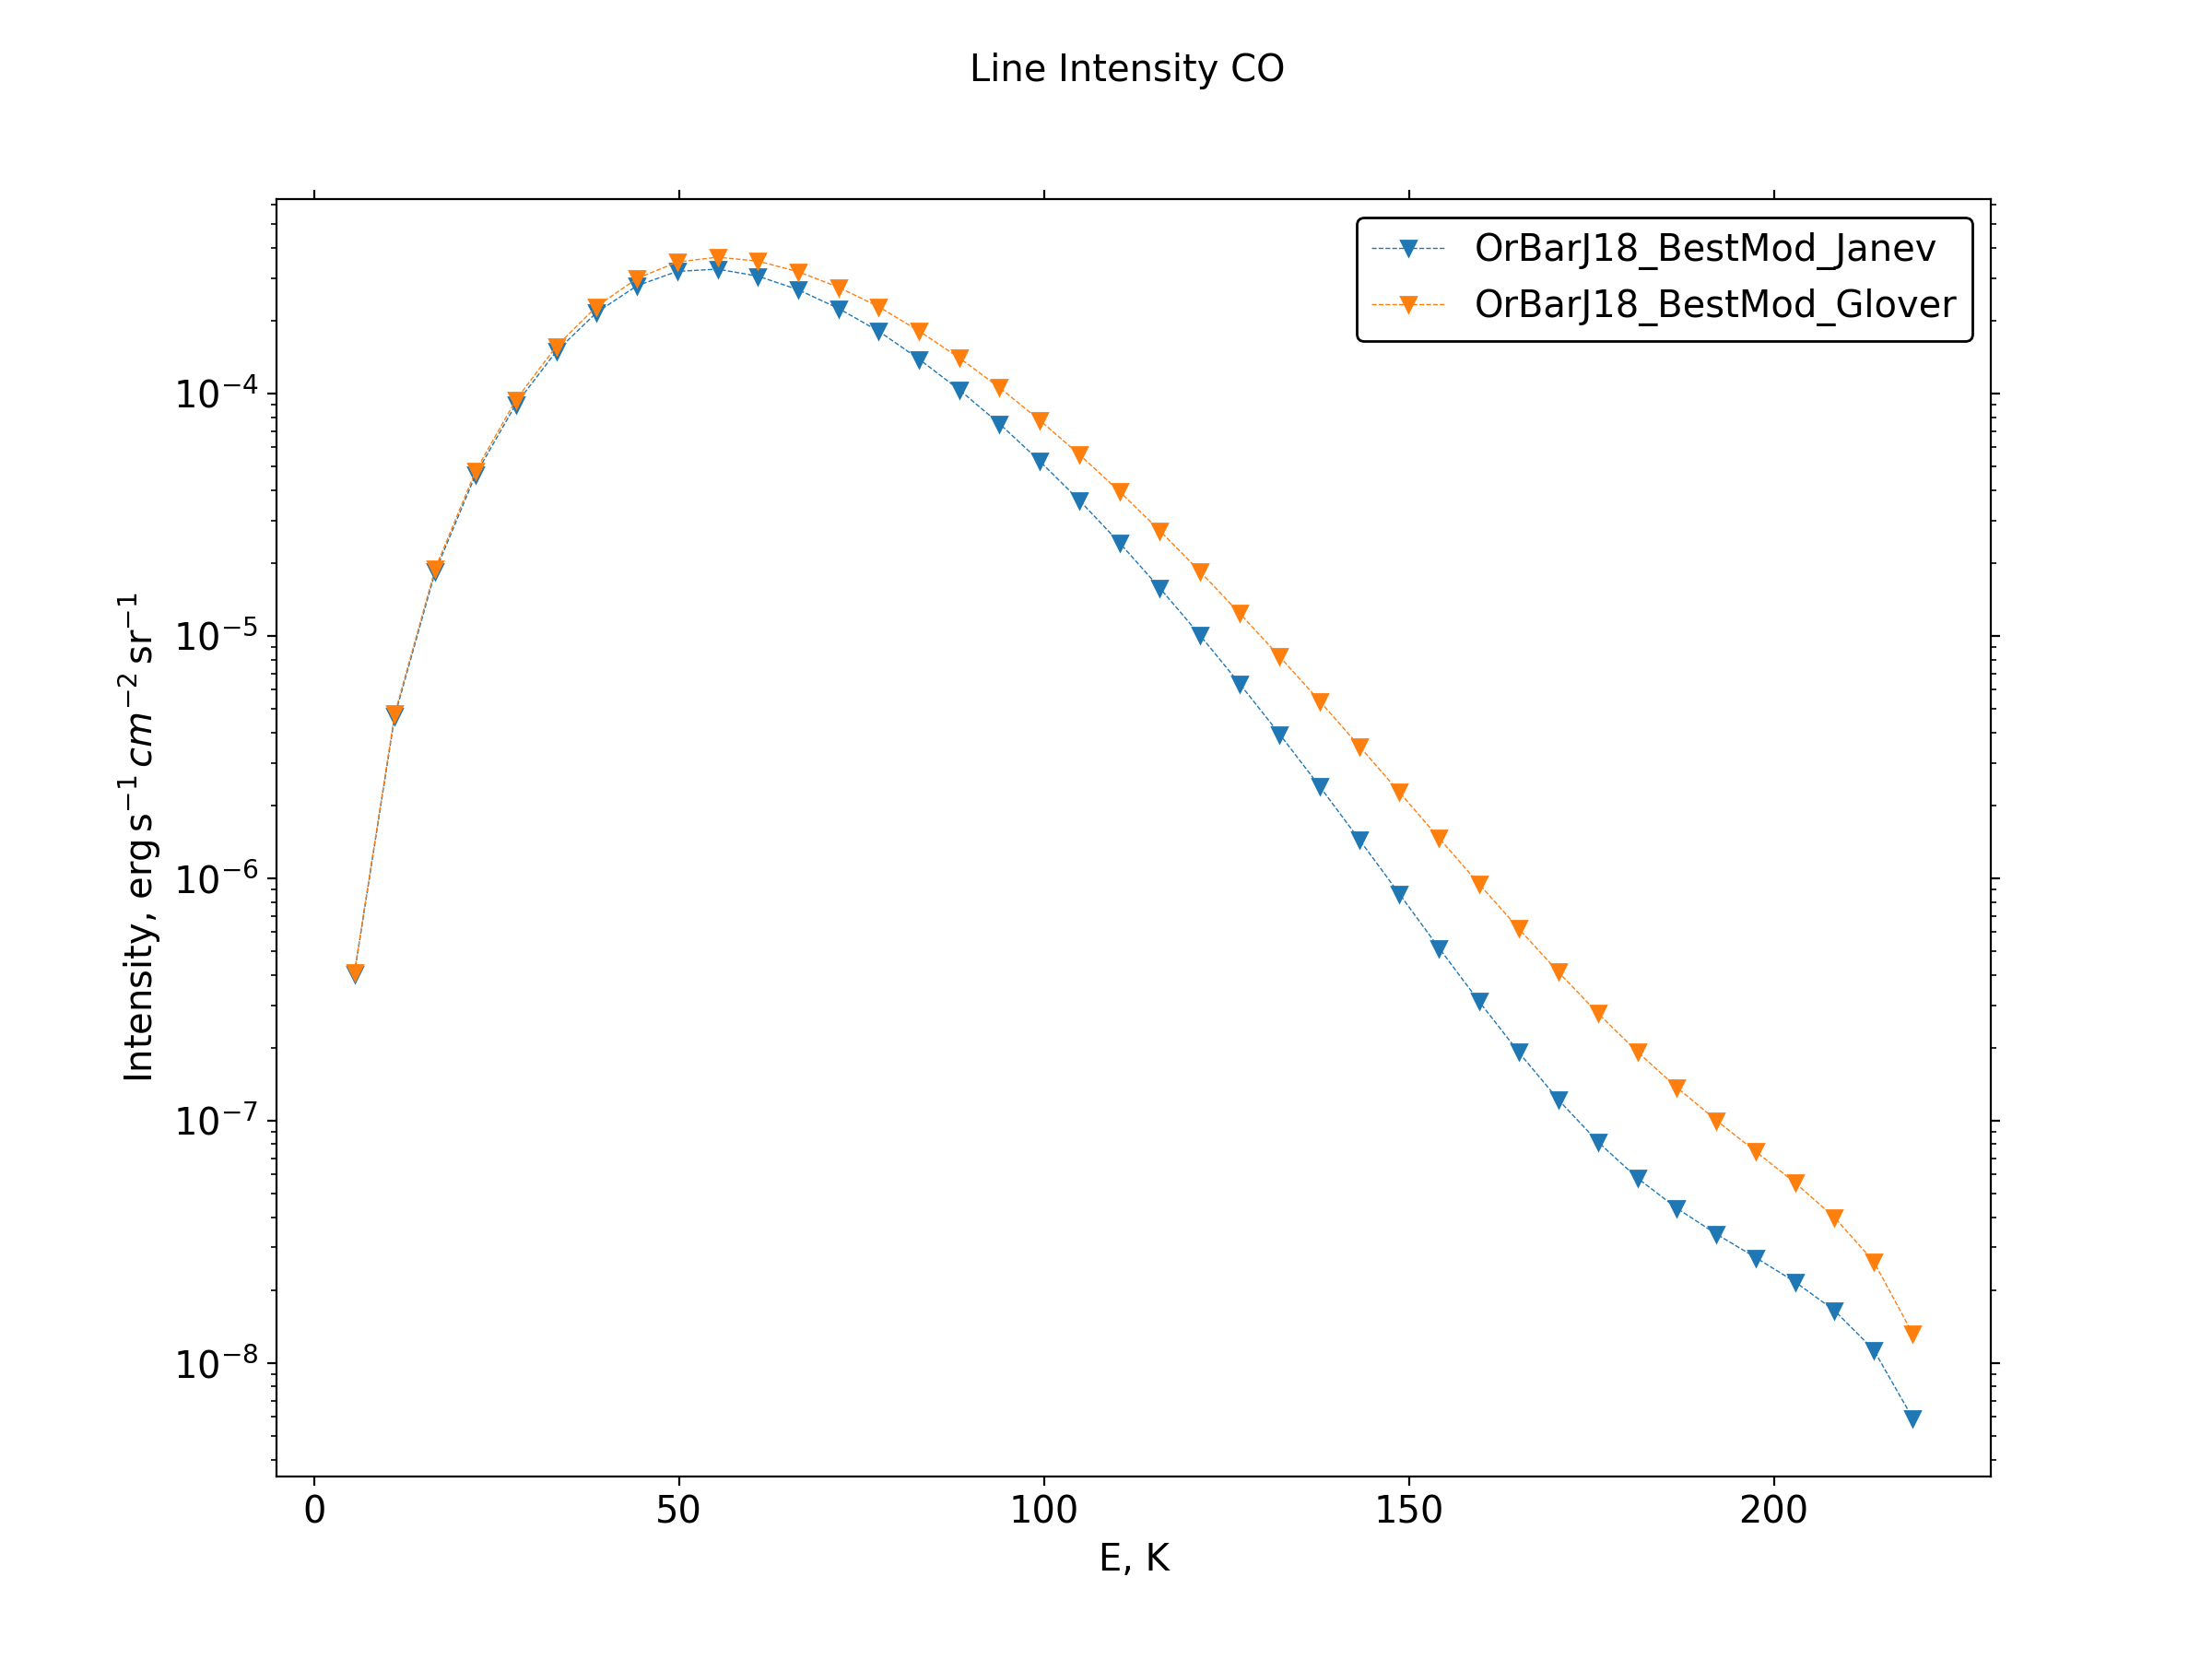
\includegraphics[trim = {0 0 0 1.5cm},clip,width=1\textwidth]{figure/H2/JanevGlover/I_comp_CO.png}
%         \caption{Spectre $\mathrm{H}_2$}
%     \end{subfigure}
%     ~ 
%     \begin{subfigure}[t]{0.49\textwidth}
%         \centering 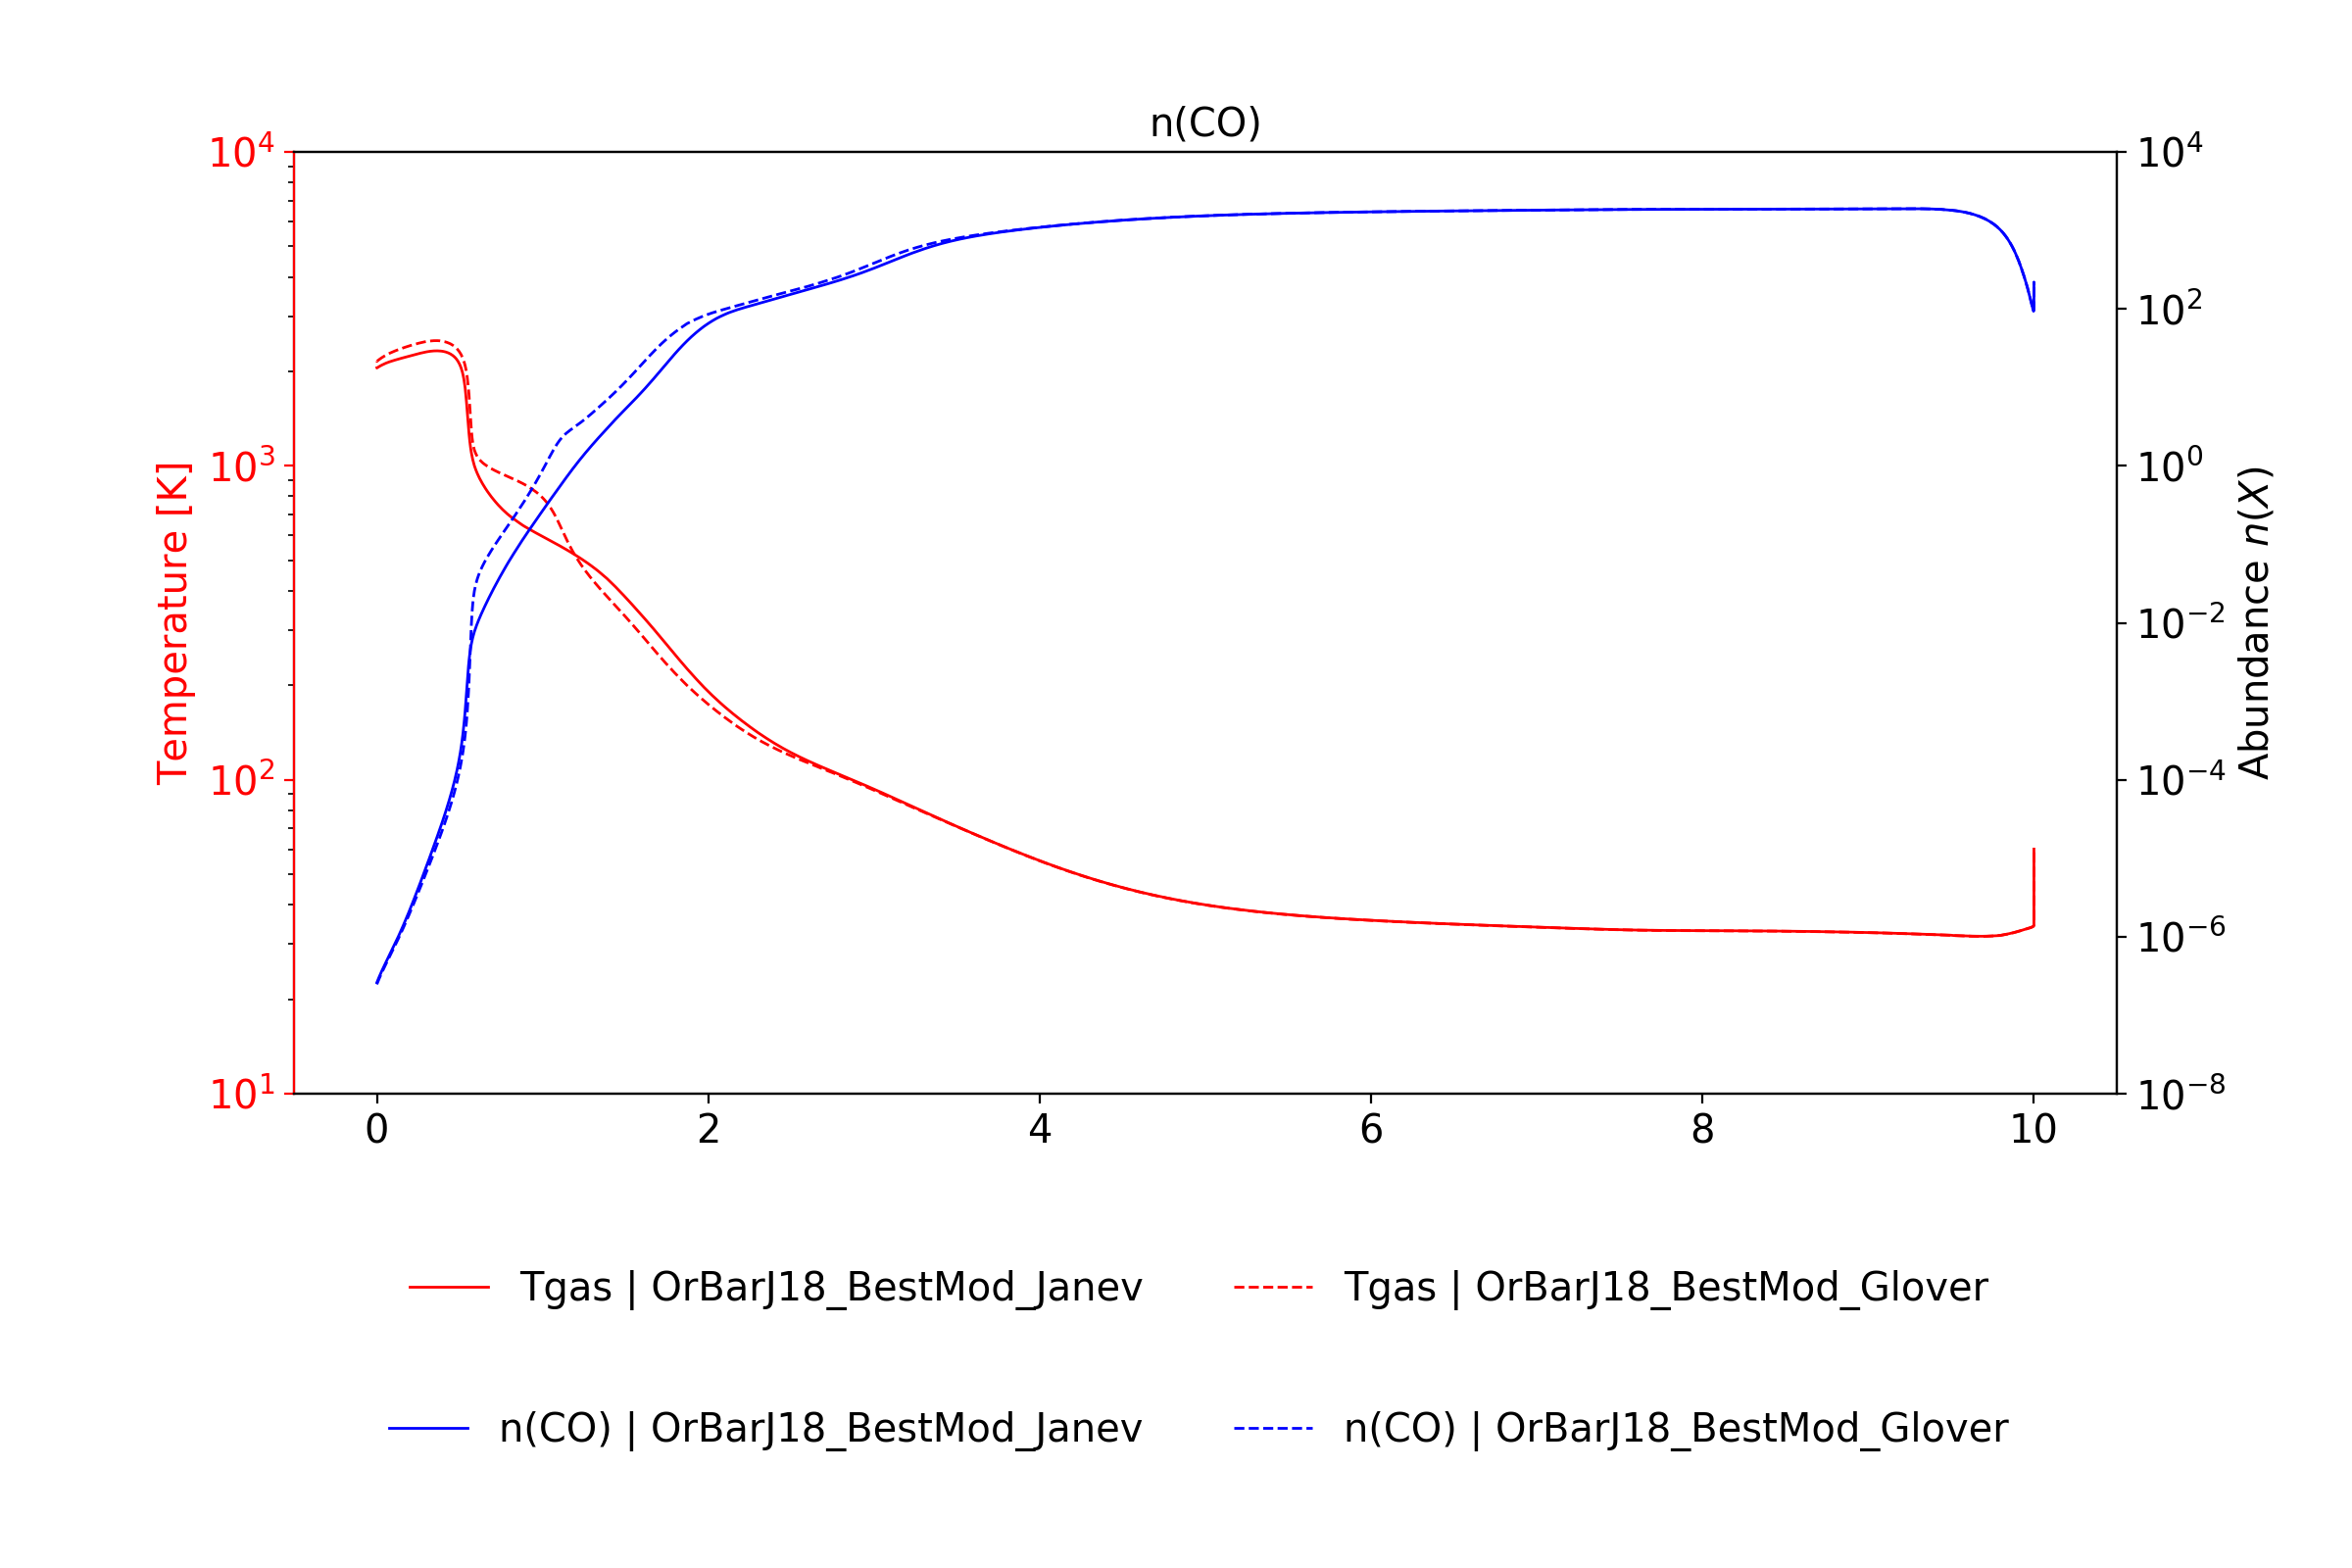
\includegraphics[trim = {0 0 0 1.5cm},clip,width=1\textwidth]{figure/H2/JanevGlover/nT_comp_CO.png}
%         \caption{Profil de densité et température de $\mathrm{H}_2$}
%     \end{subfigure}

%     \centering
%     \begin{subfigure}[t]{0.49\textwidth} % "0.49" donne ici la largeur de l'image
%         \centering 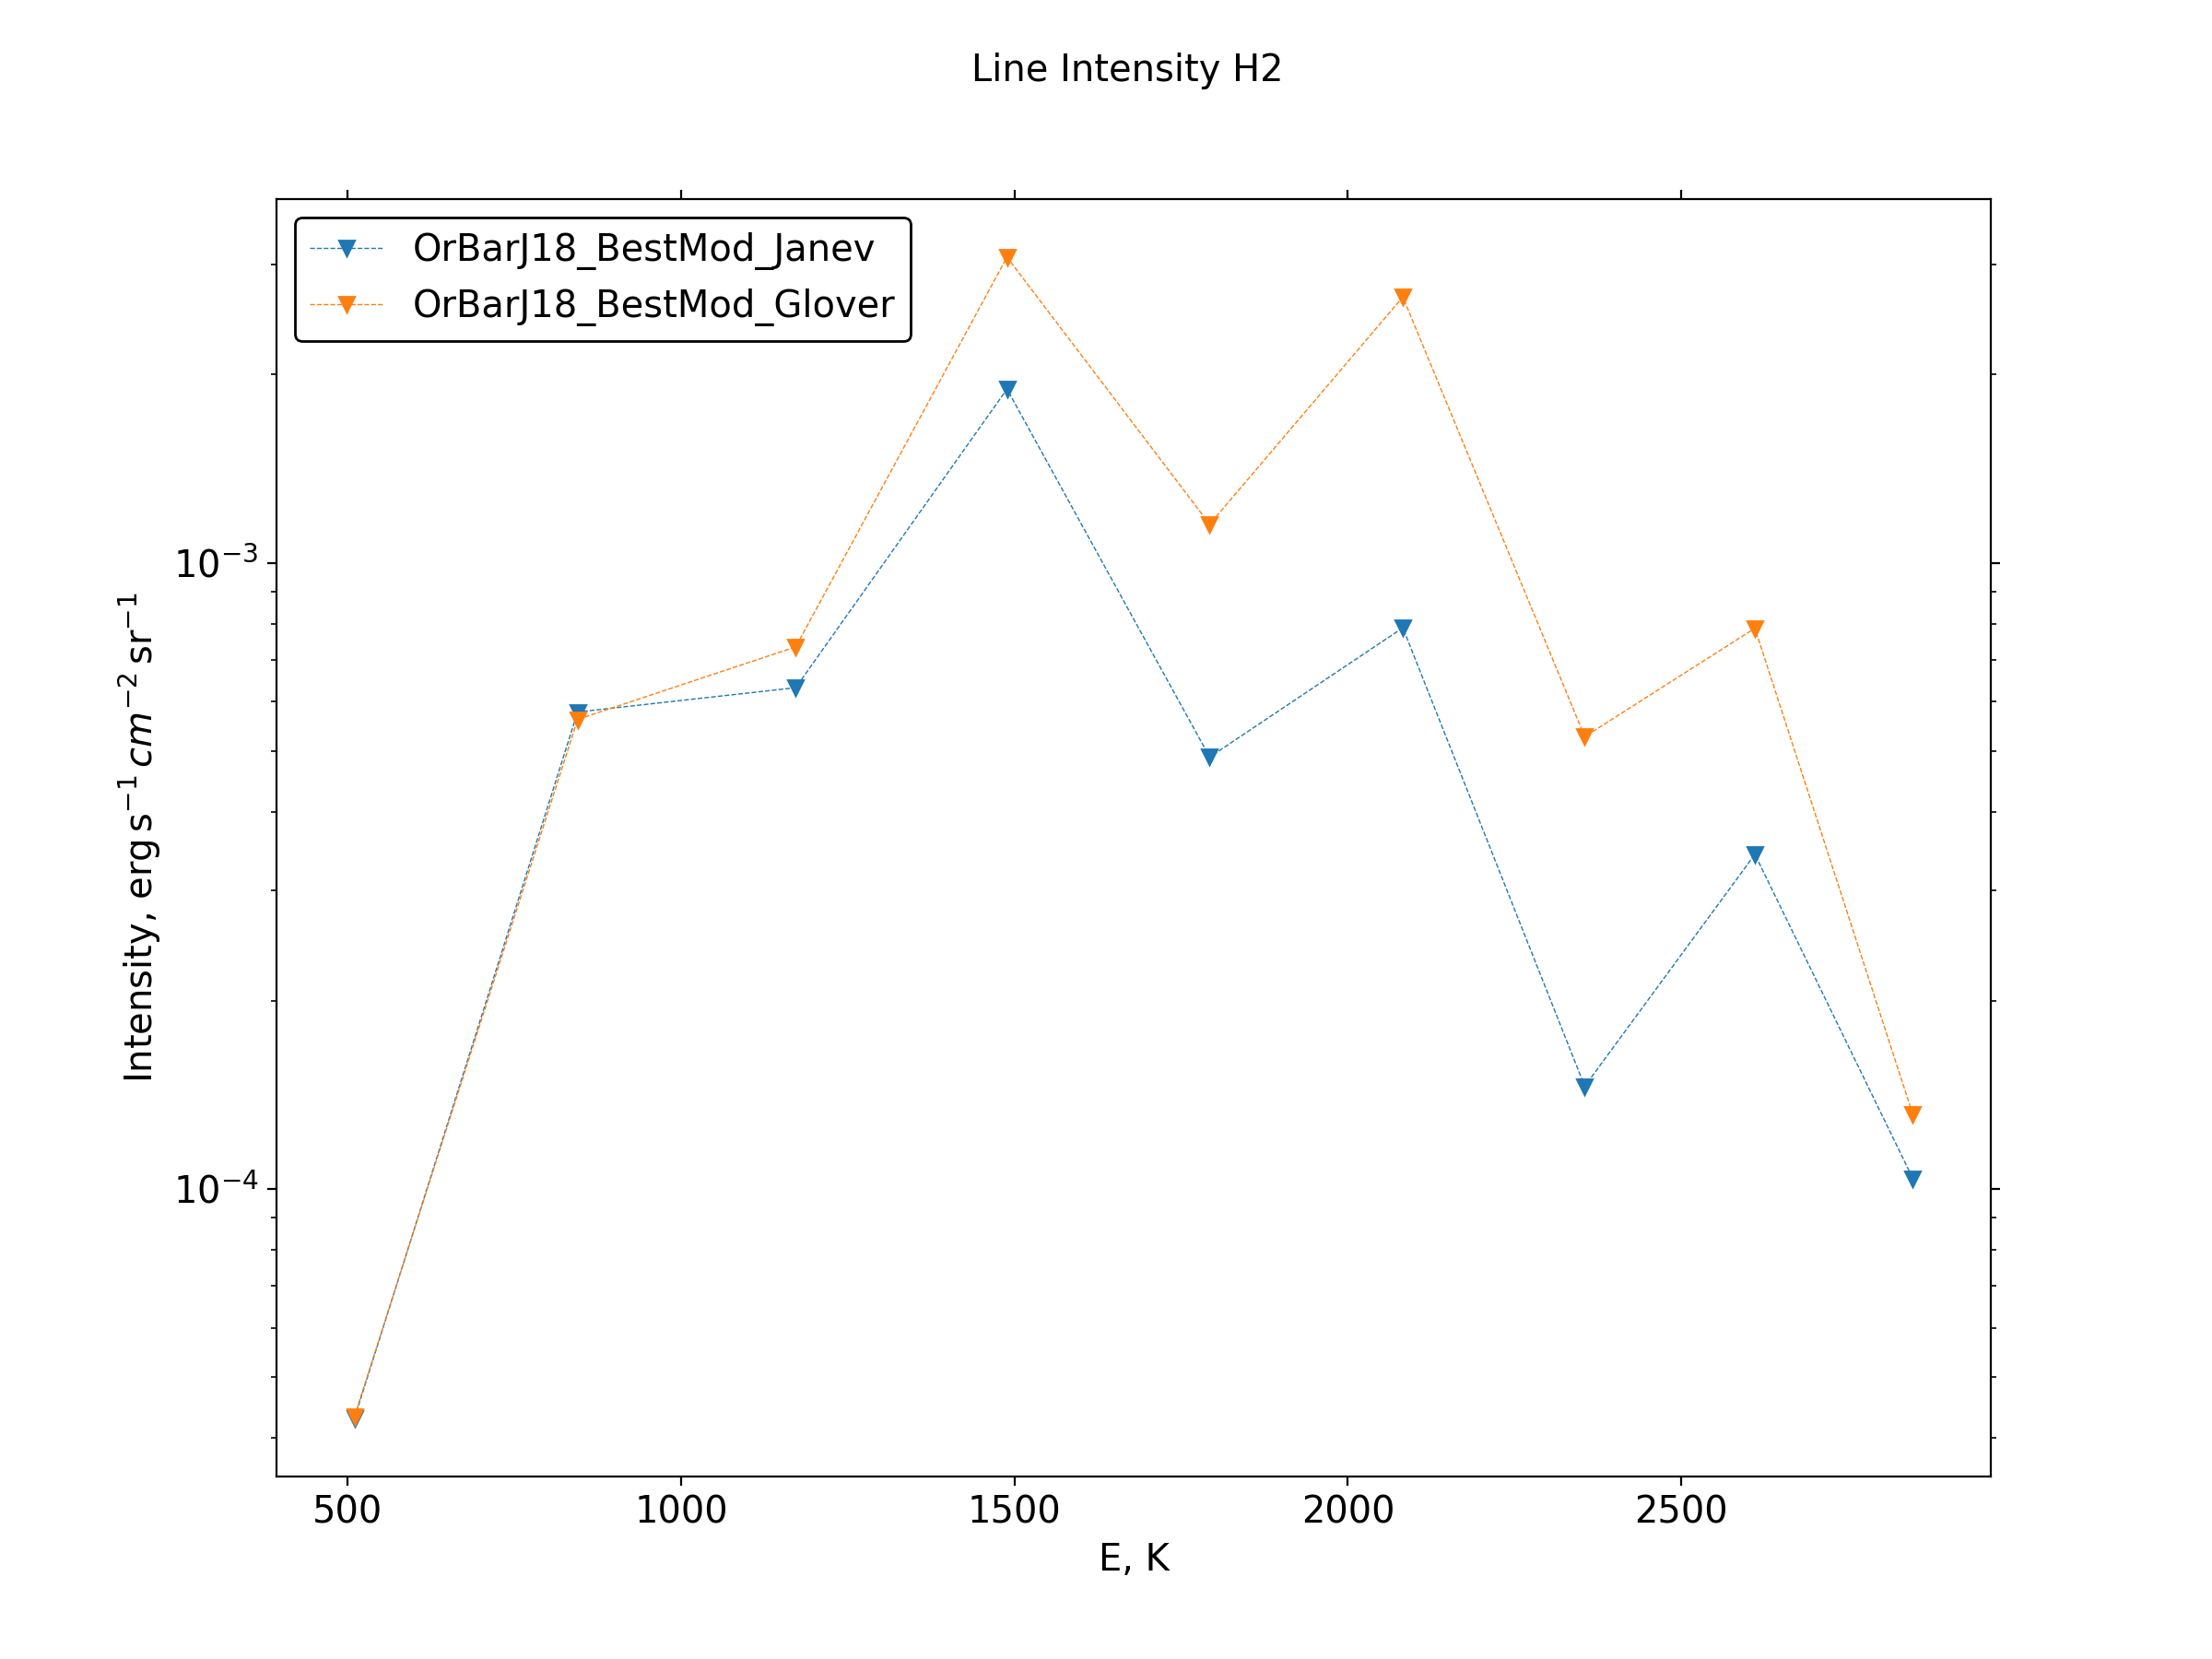
\includegraphics[trim = {0 0 0 1.5cm},clip,width=1\textwidth]{figure/H2/JanevGlover/I_comp_H2.png}
%         \caption{Spectre de $\mathrm{CO}$}
%     \end{subfigure}
%     ~ 
%     \begin{subfigure}[t]{0.49\textwidth}
%         \centering 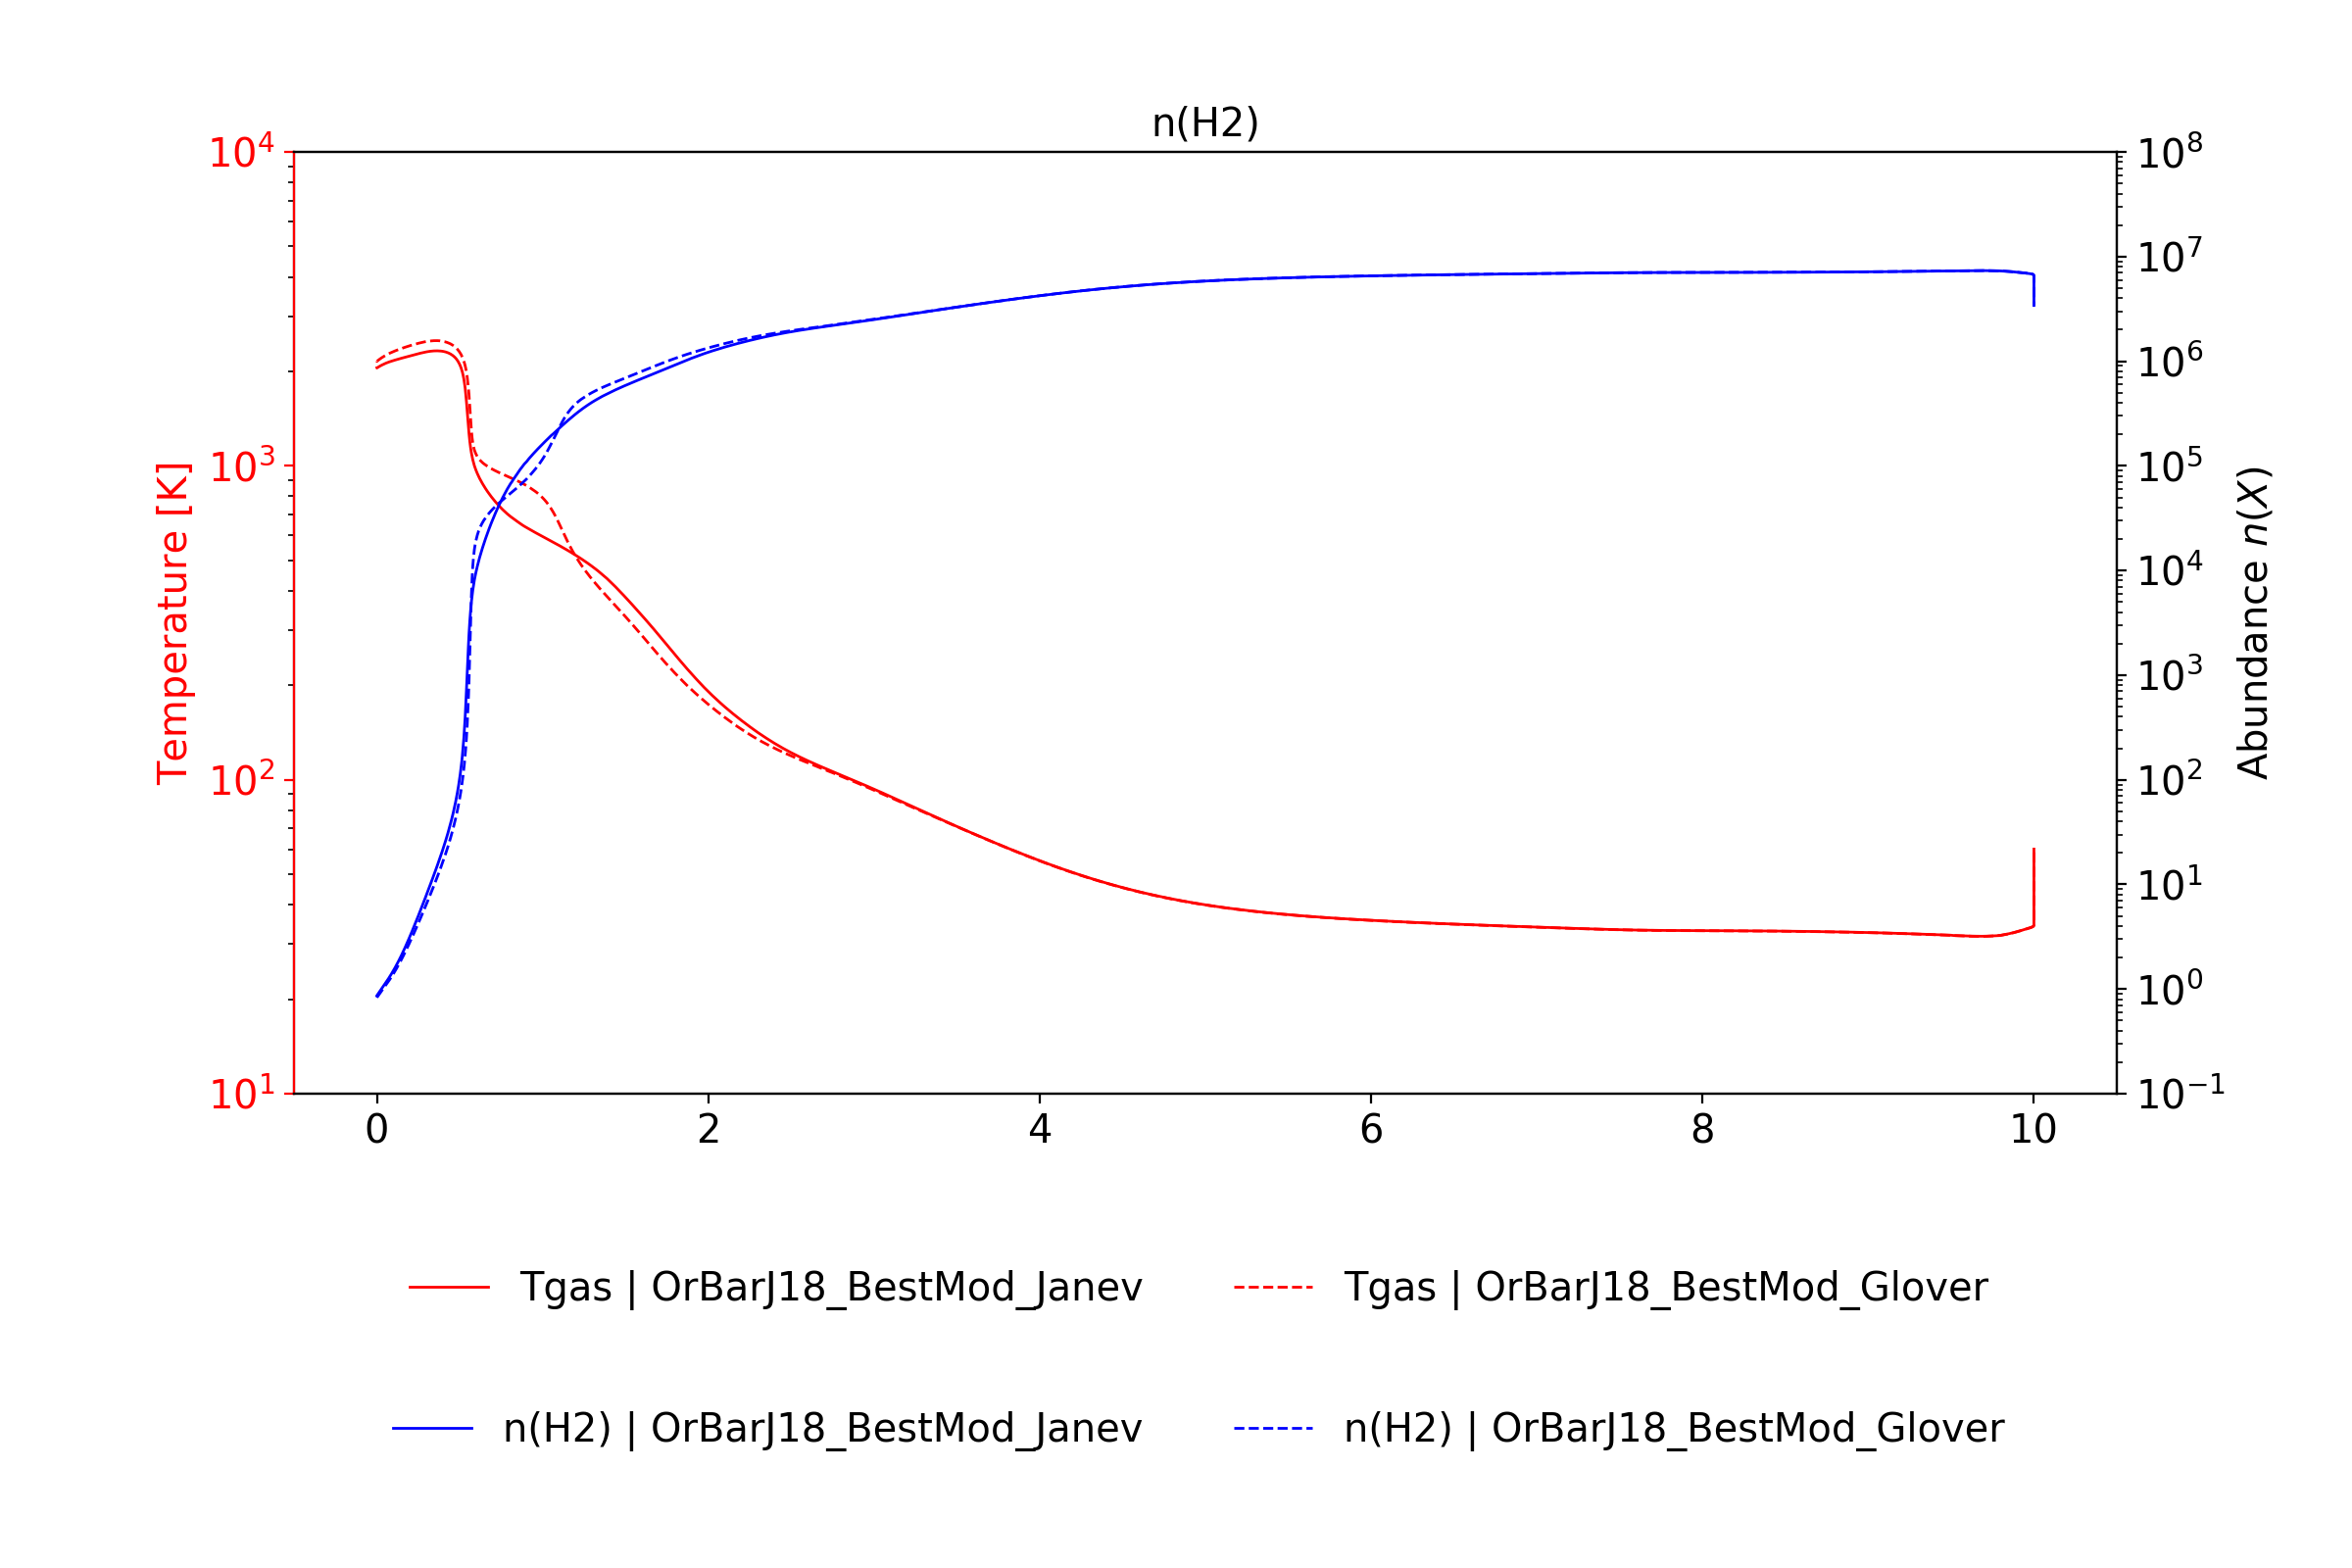
\includegraphics[trim = {0 0 0 1.5cm},clip,width=1\textwidth]{figure/H2/JanevGlover/nT_comp_H2.png}
%         \caption{Profil de densité et température de $\mathrm{CO}$}
%     \end{subfigure}
%     \caption{Impact des prescriptions de Janev et Glover sur les raies d'émissions des traceurs $\mathrm{H}_2$ et $\mathrm{CO}$}
%     \label{fig:H2:JanevGlover:emiss}
% \end{figure}


% Néanmoins on connaît mal la proportion effective qui chauffe le gaz par exothermicité. Il faut reprendre l'étude sur l'exothermicité des réactions chimiques en jouant sur la prescription. \newline 

% On cherche à visualiser l'impact des nouveaux calculs des niveaux de $\mathrm{H}_2$ sur les raies. On l'a calculé dans le cas de Janev et Glover mais l'on montre seulement la prescription de Glover qui est la plus importante (\autoref{fig:H2:GloverBossion:emiss})

% On se rend compte que l'impact est minime alors que le travail pour calculer ces niveaux est lourd. Au moins on sait que connaître précisément les niveaux de $\mathrm{H}_2$ n'est pas décisif dans l'interprétation des spectres d'émissions. 

% \begin{figure}[h!]
%     \centering
%     \begin{subfigure}[t]{0.49\textwidth} % "0.49" donne ici la largeur de l'image
%         \centering 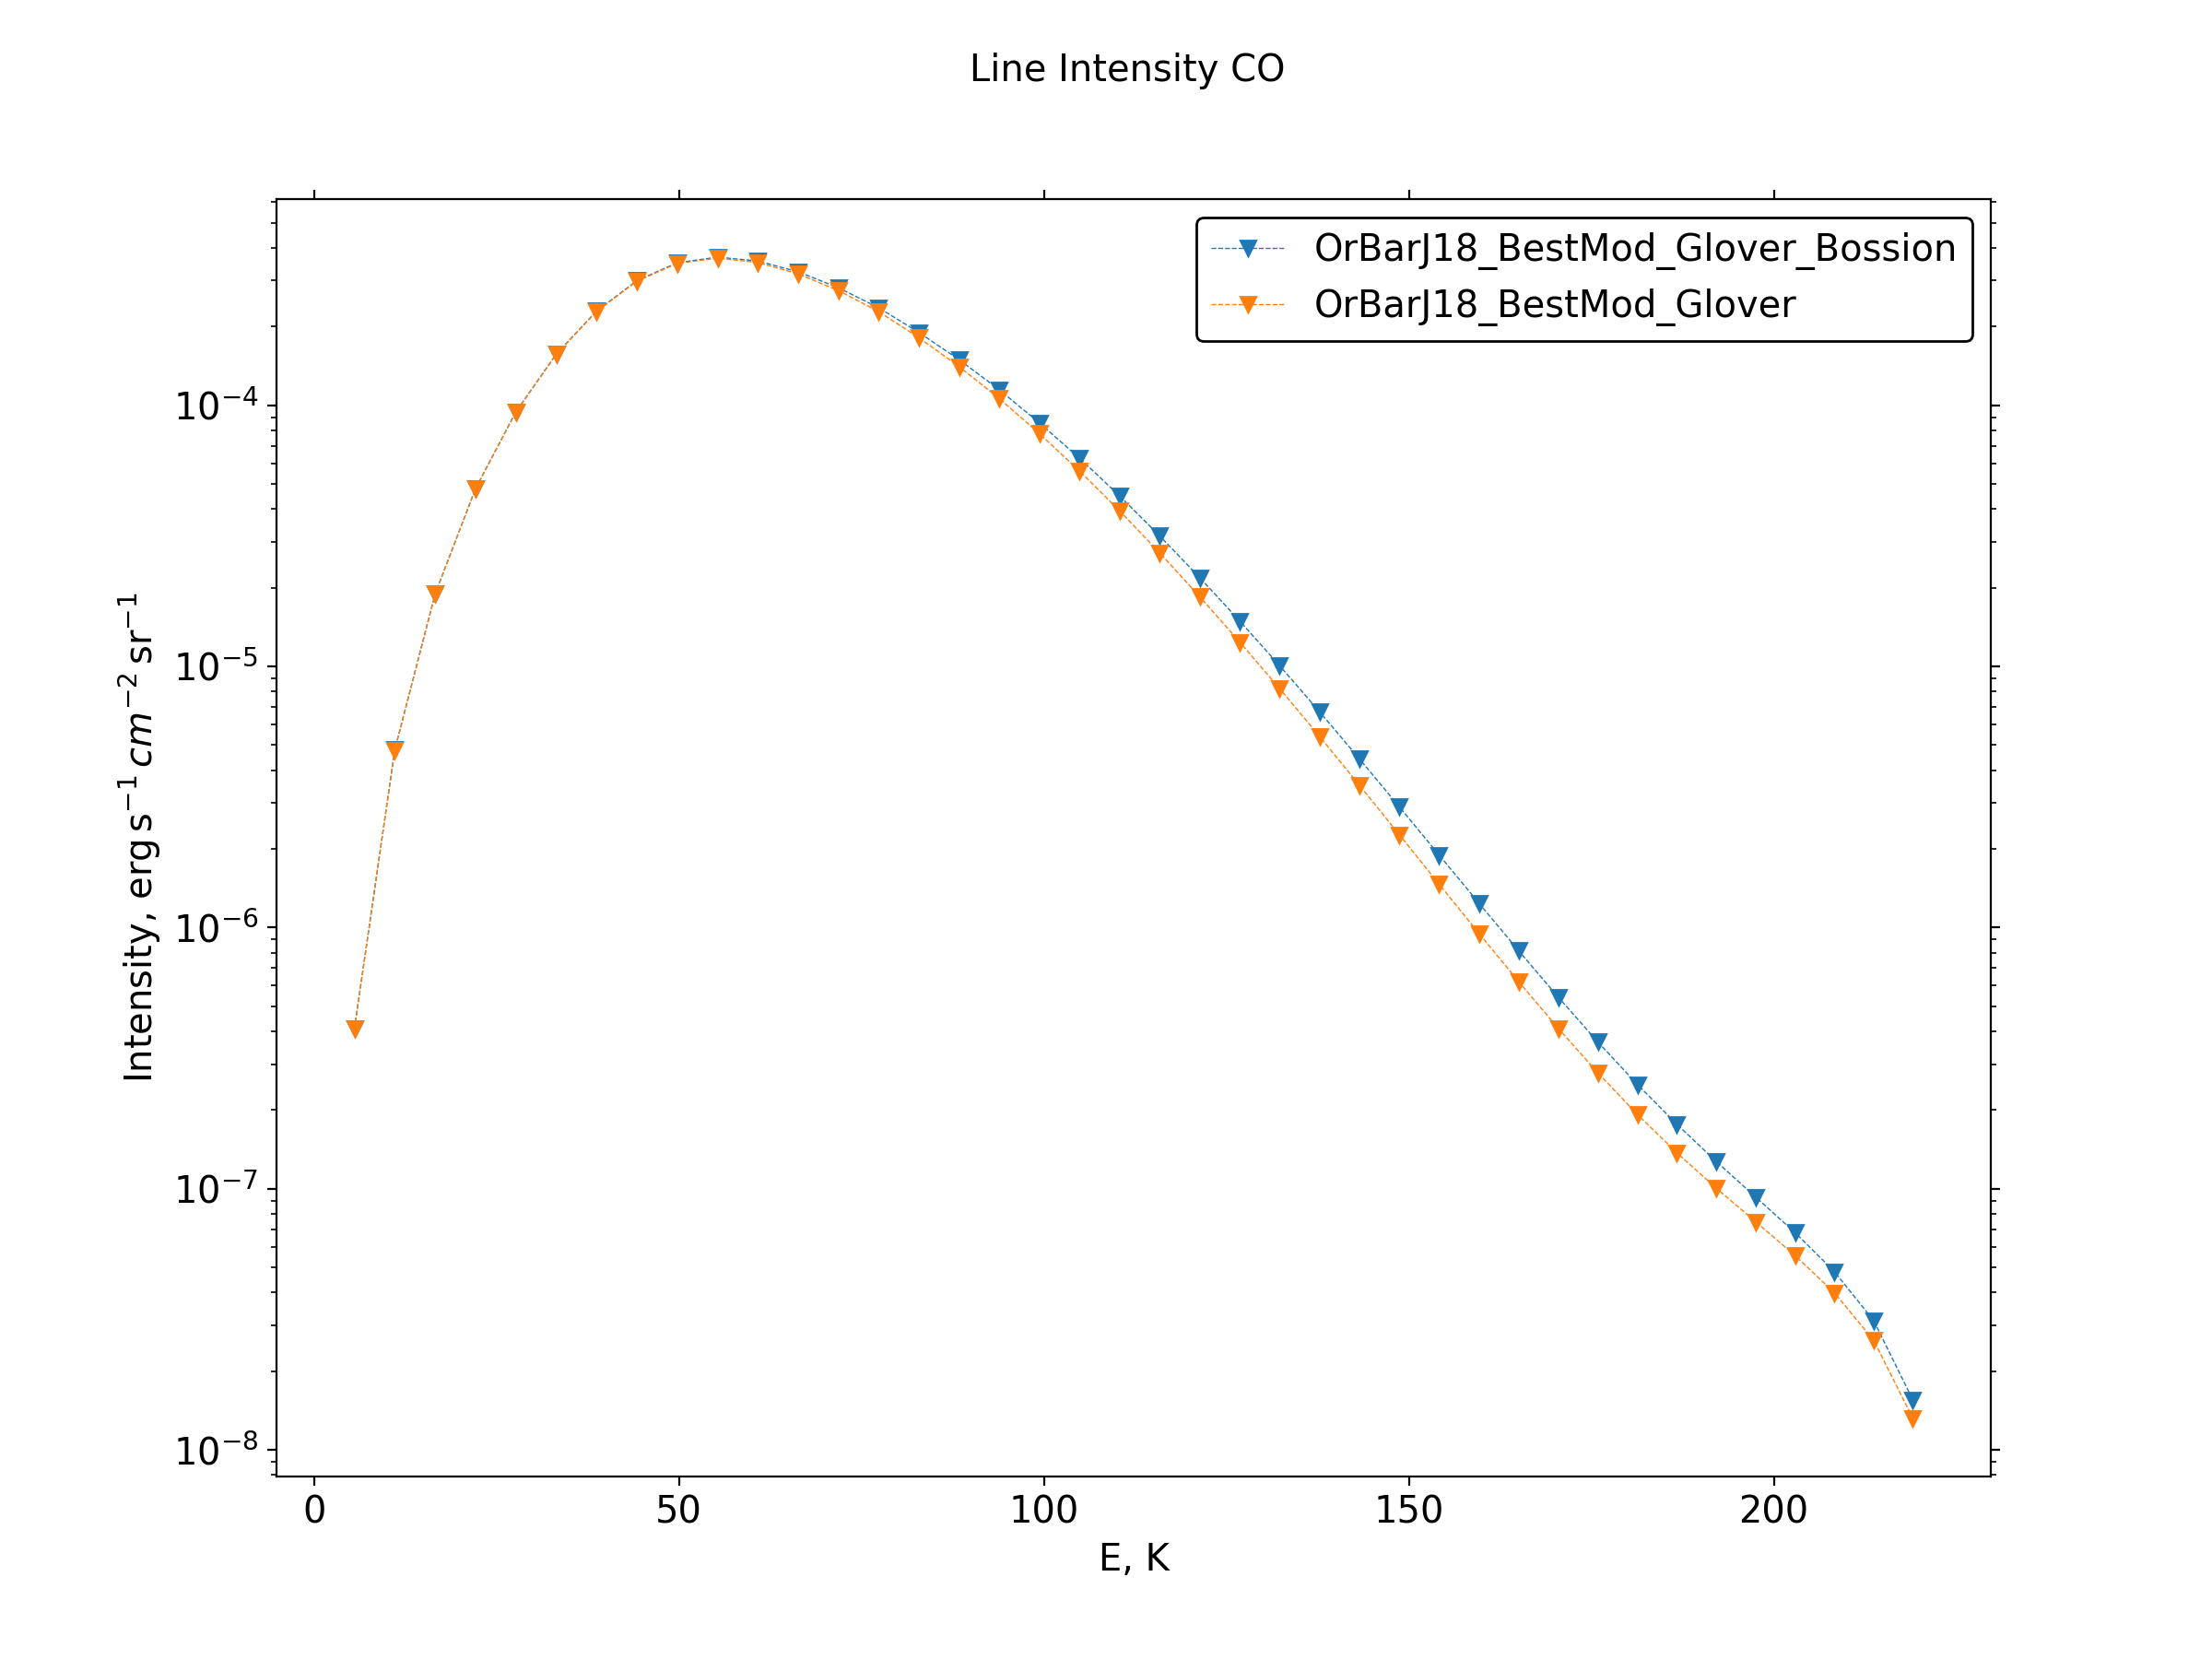
\includegraphics[trim = {0 0 0 1.5cm},clip,width=1\textwidth]{figure/H2/GloverBossion/I_comp_CO.png}
%         \caption{Spectre $\mathrm{H}_2$}
%     \end{subfigure}
%     ~ 
%     \begin{subfigure}[t]{0.49\textwidth}
%         \centering 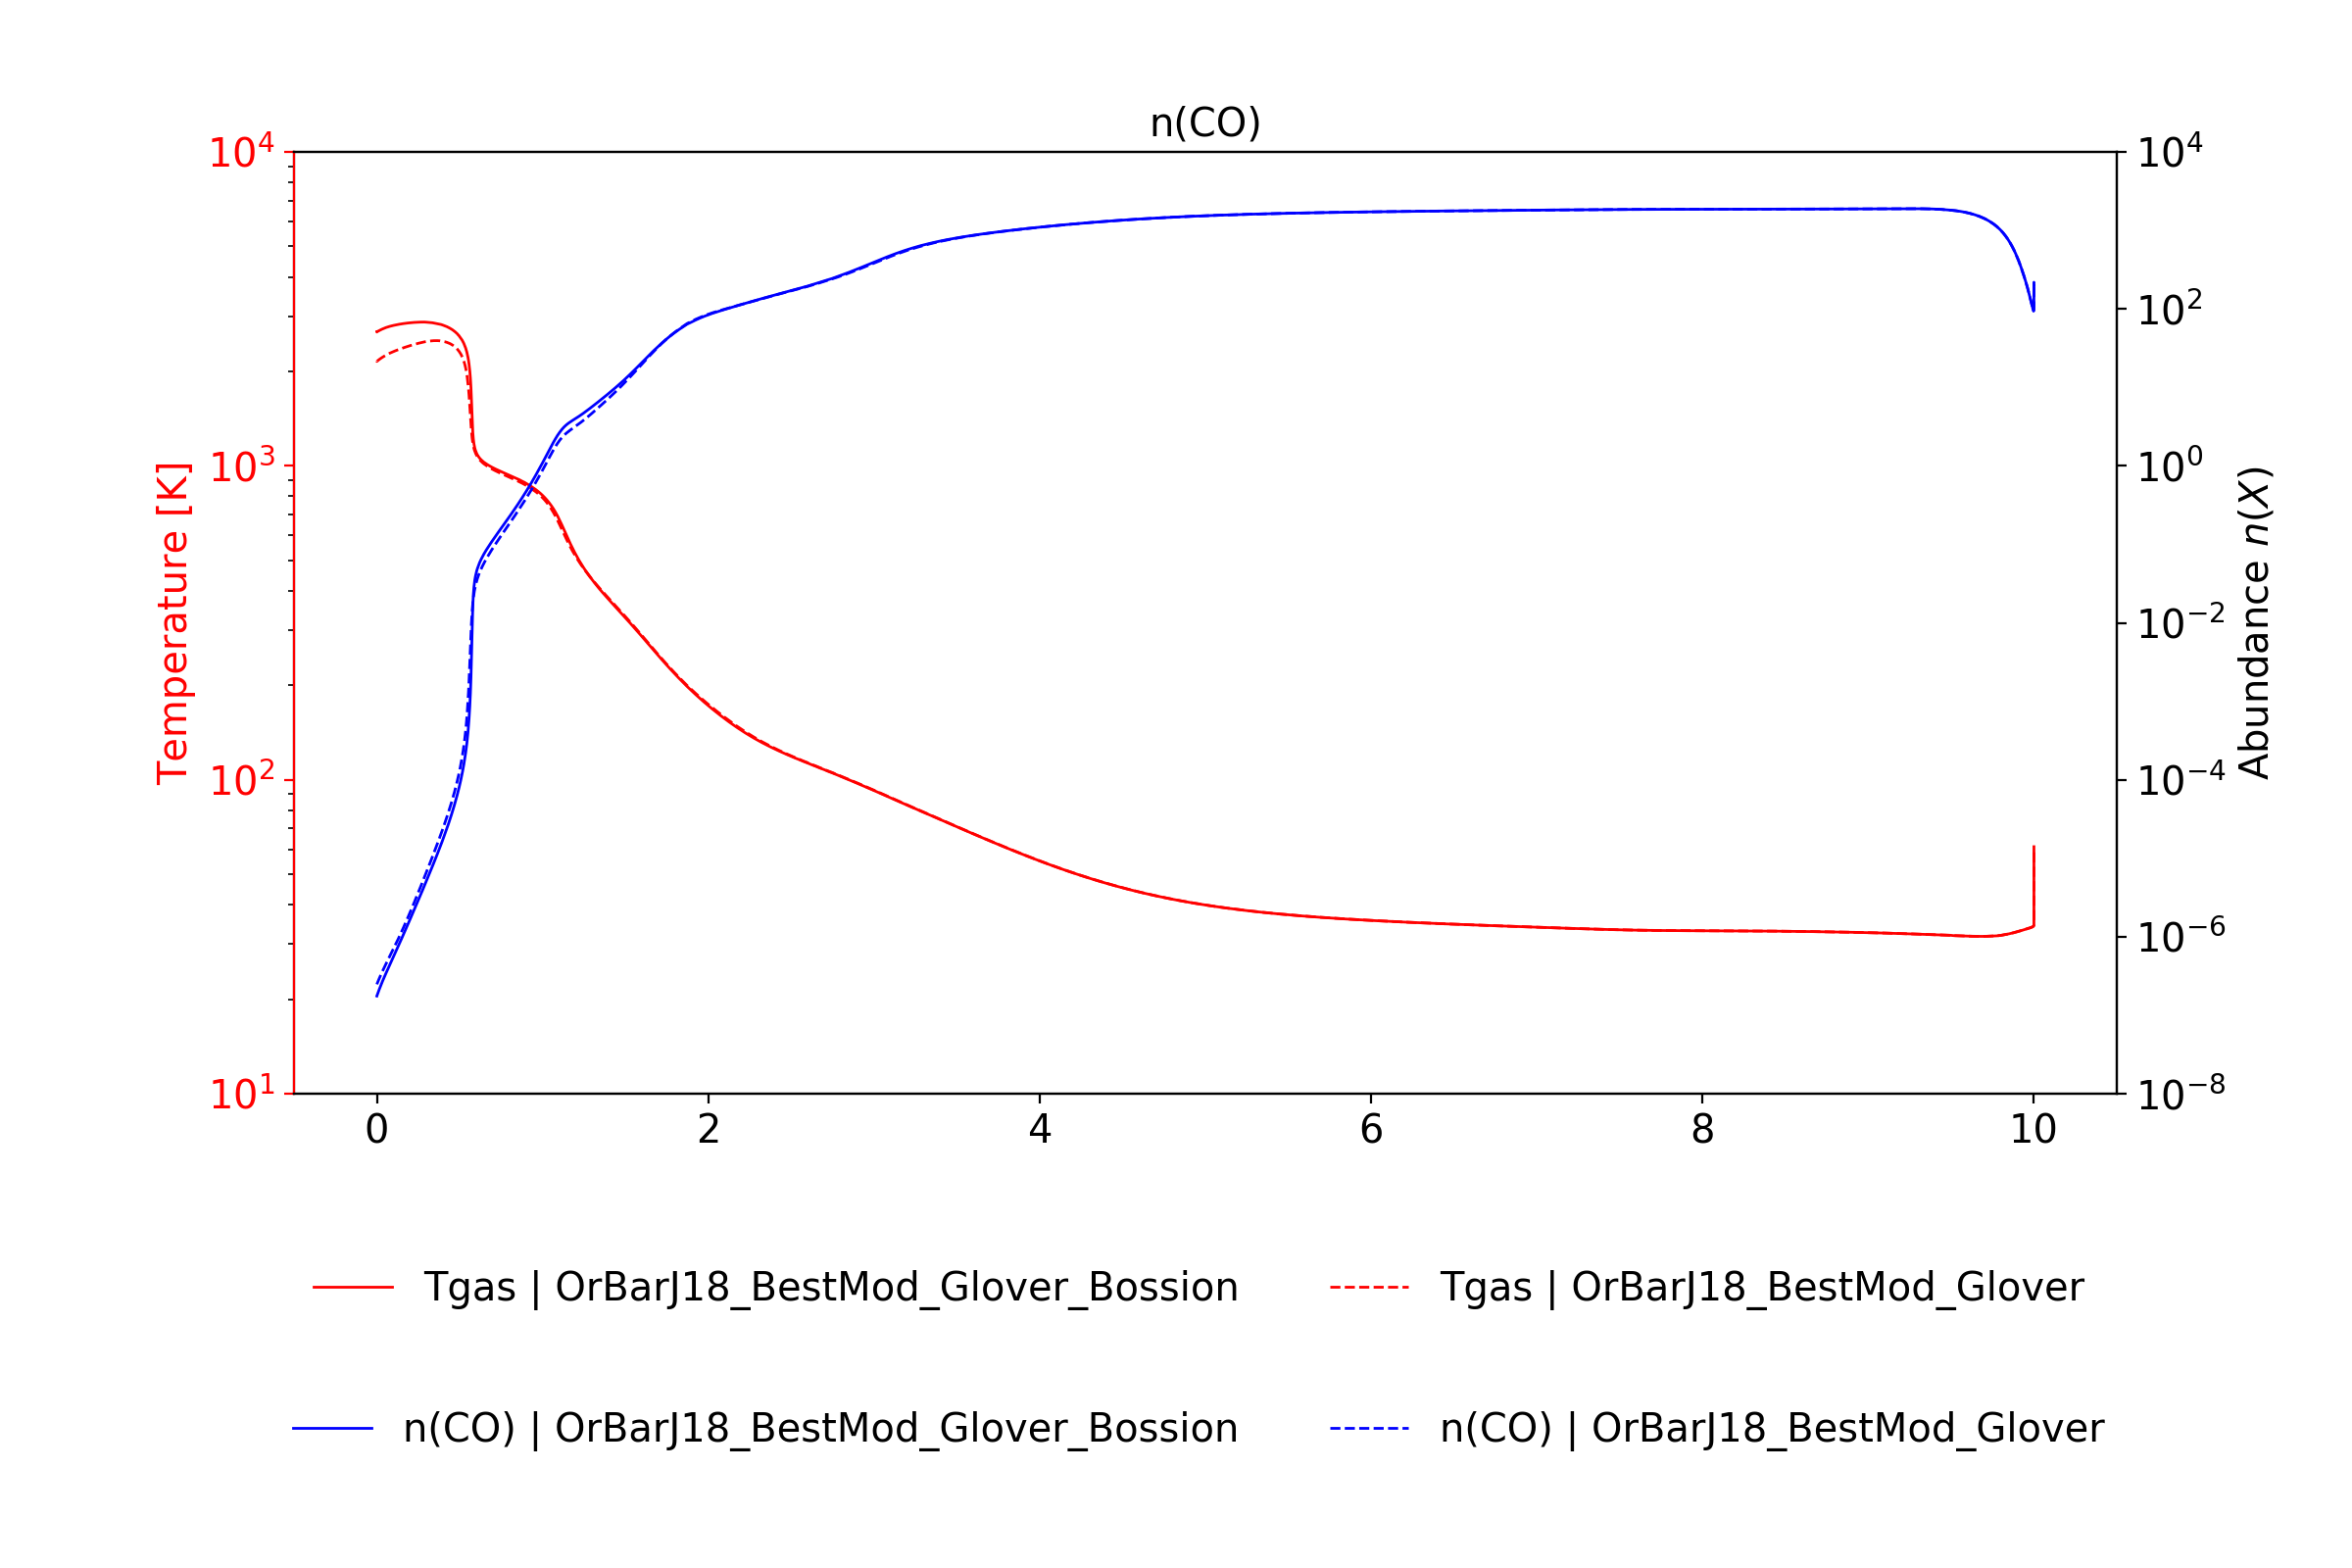
\includegraphics[trim = {0 0 0 1.5cm},clip,width=1\textwidth]{figure/H2/GloverBossion/nT_comp_CO.png}
%         \caption{Profil de densité et température de $\mathrm{H}_2$}
%     \end{subfigure}

%     \centering
%     \begin{subfigure}[t]{0.49\textwidth} % "0.49" donne ici la largeur de l'image
%         \centering 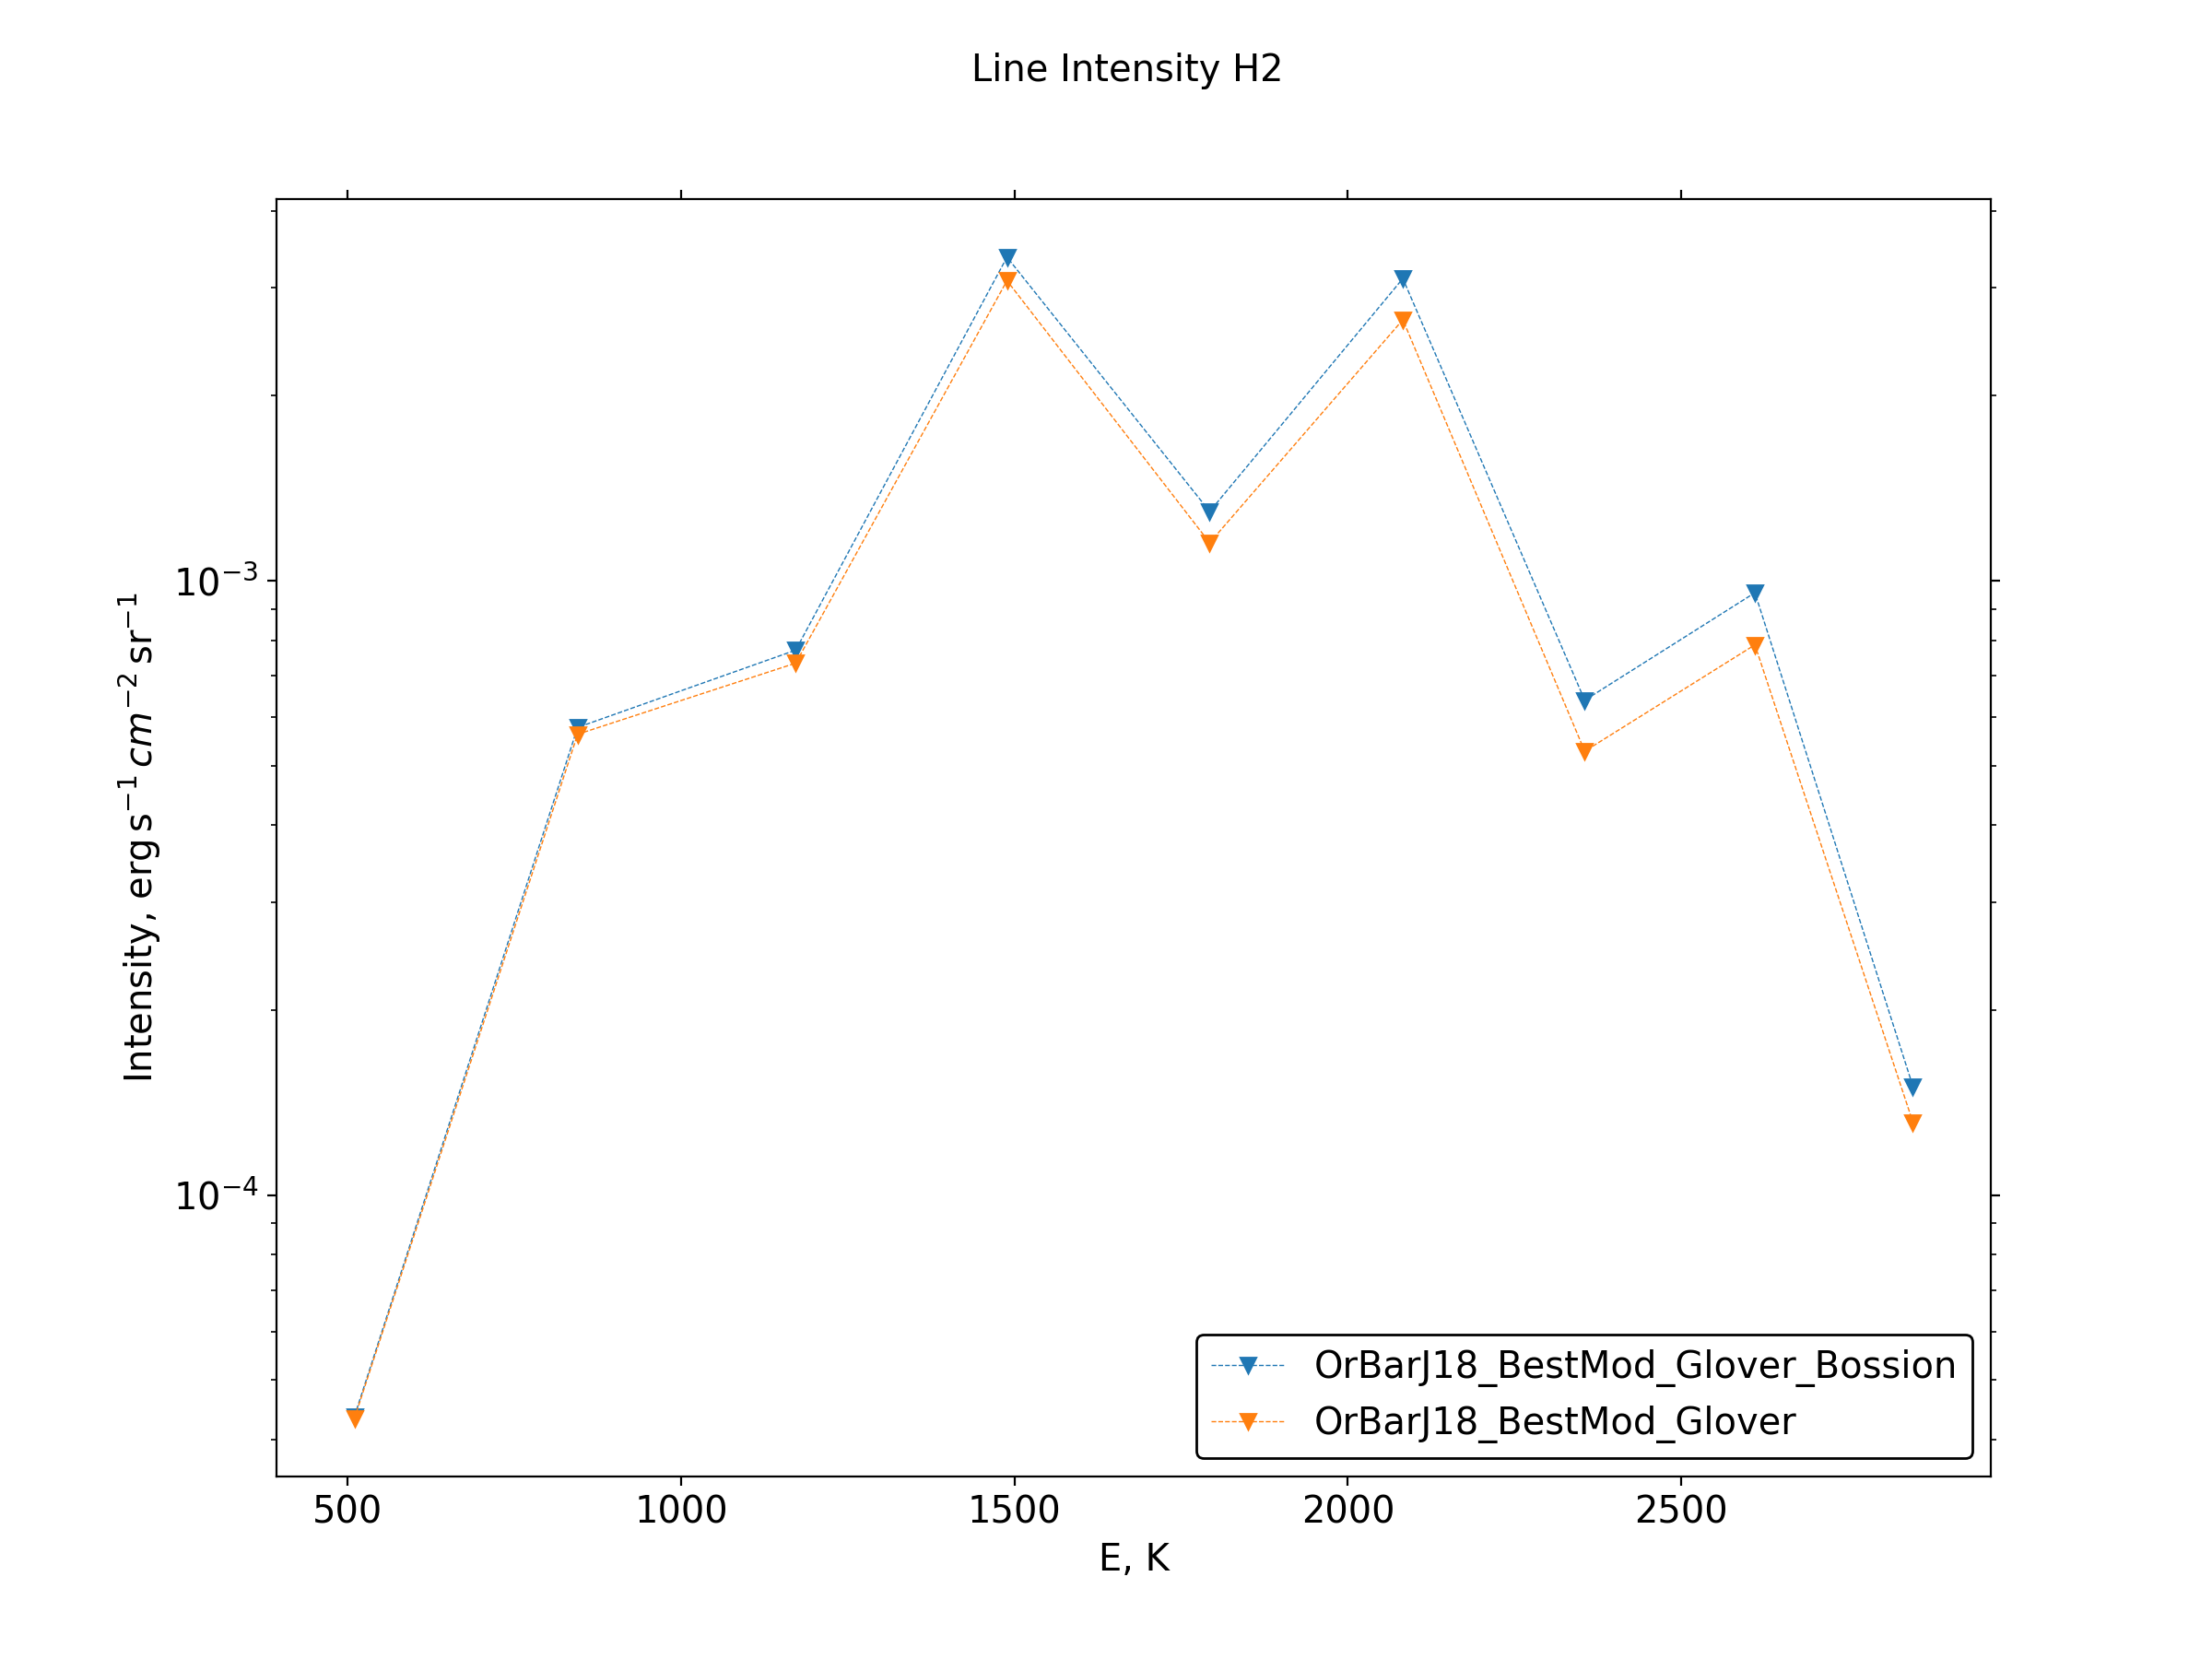
\includegraphics[trim = {0 0 0 1.5cm},clip,width=1\textwidth]{figure/H2/GloverBossion/I_comp_H2.png}
%         \caption{Spectre de $\mathrm{CO}$}
%     \end{subfigure}
%     ~ 
%     \begin{subfigure}[t]{0.49\textwidth}
%         \centering 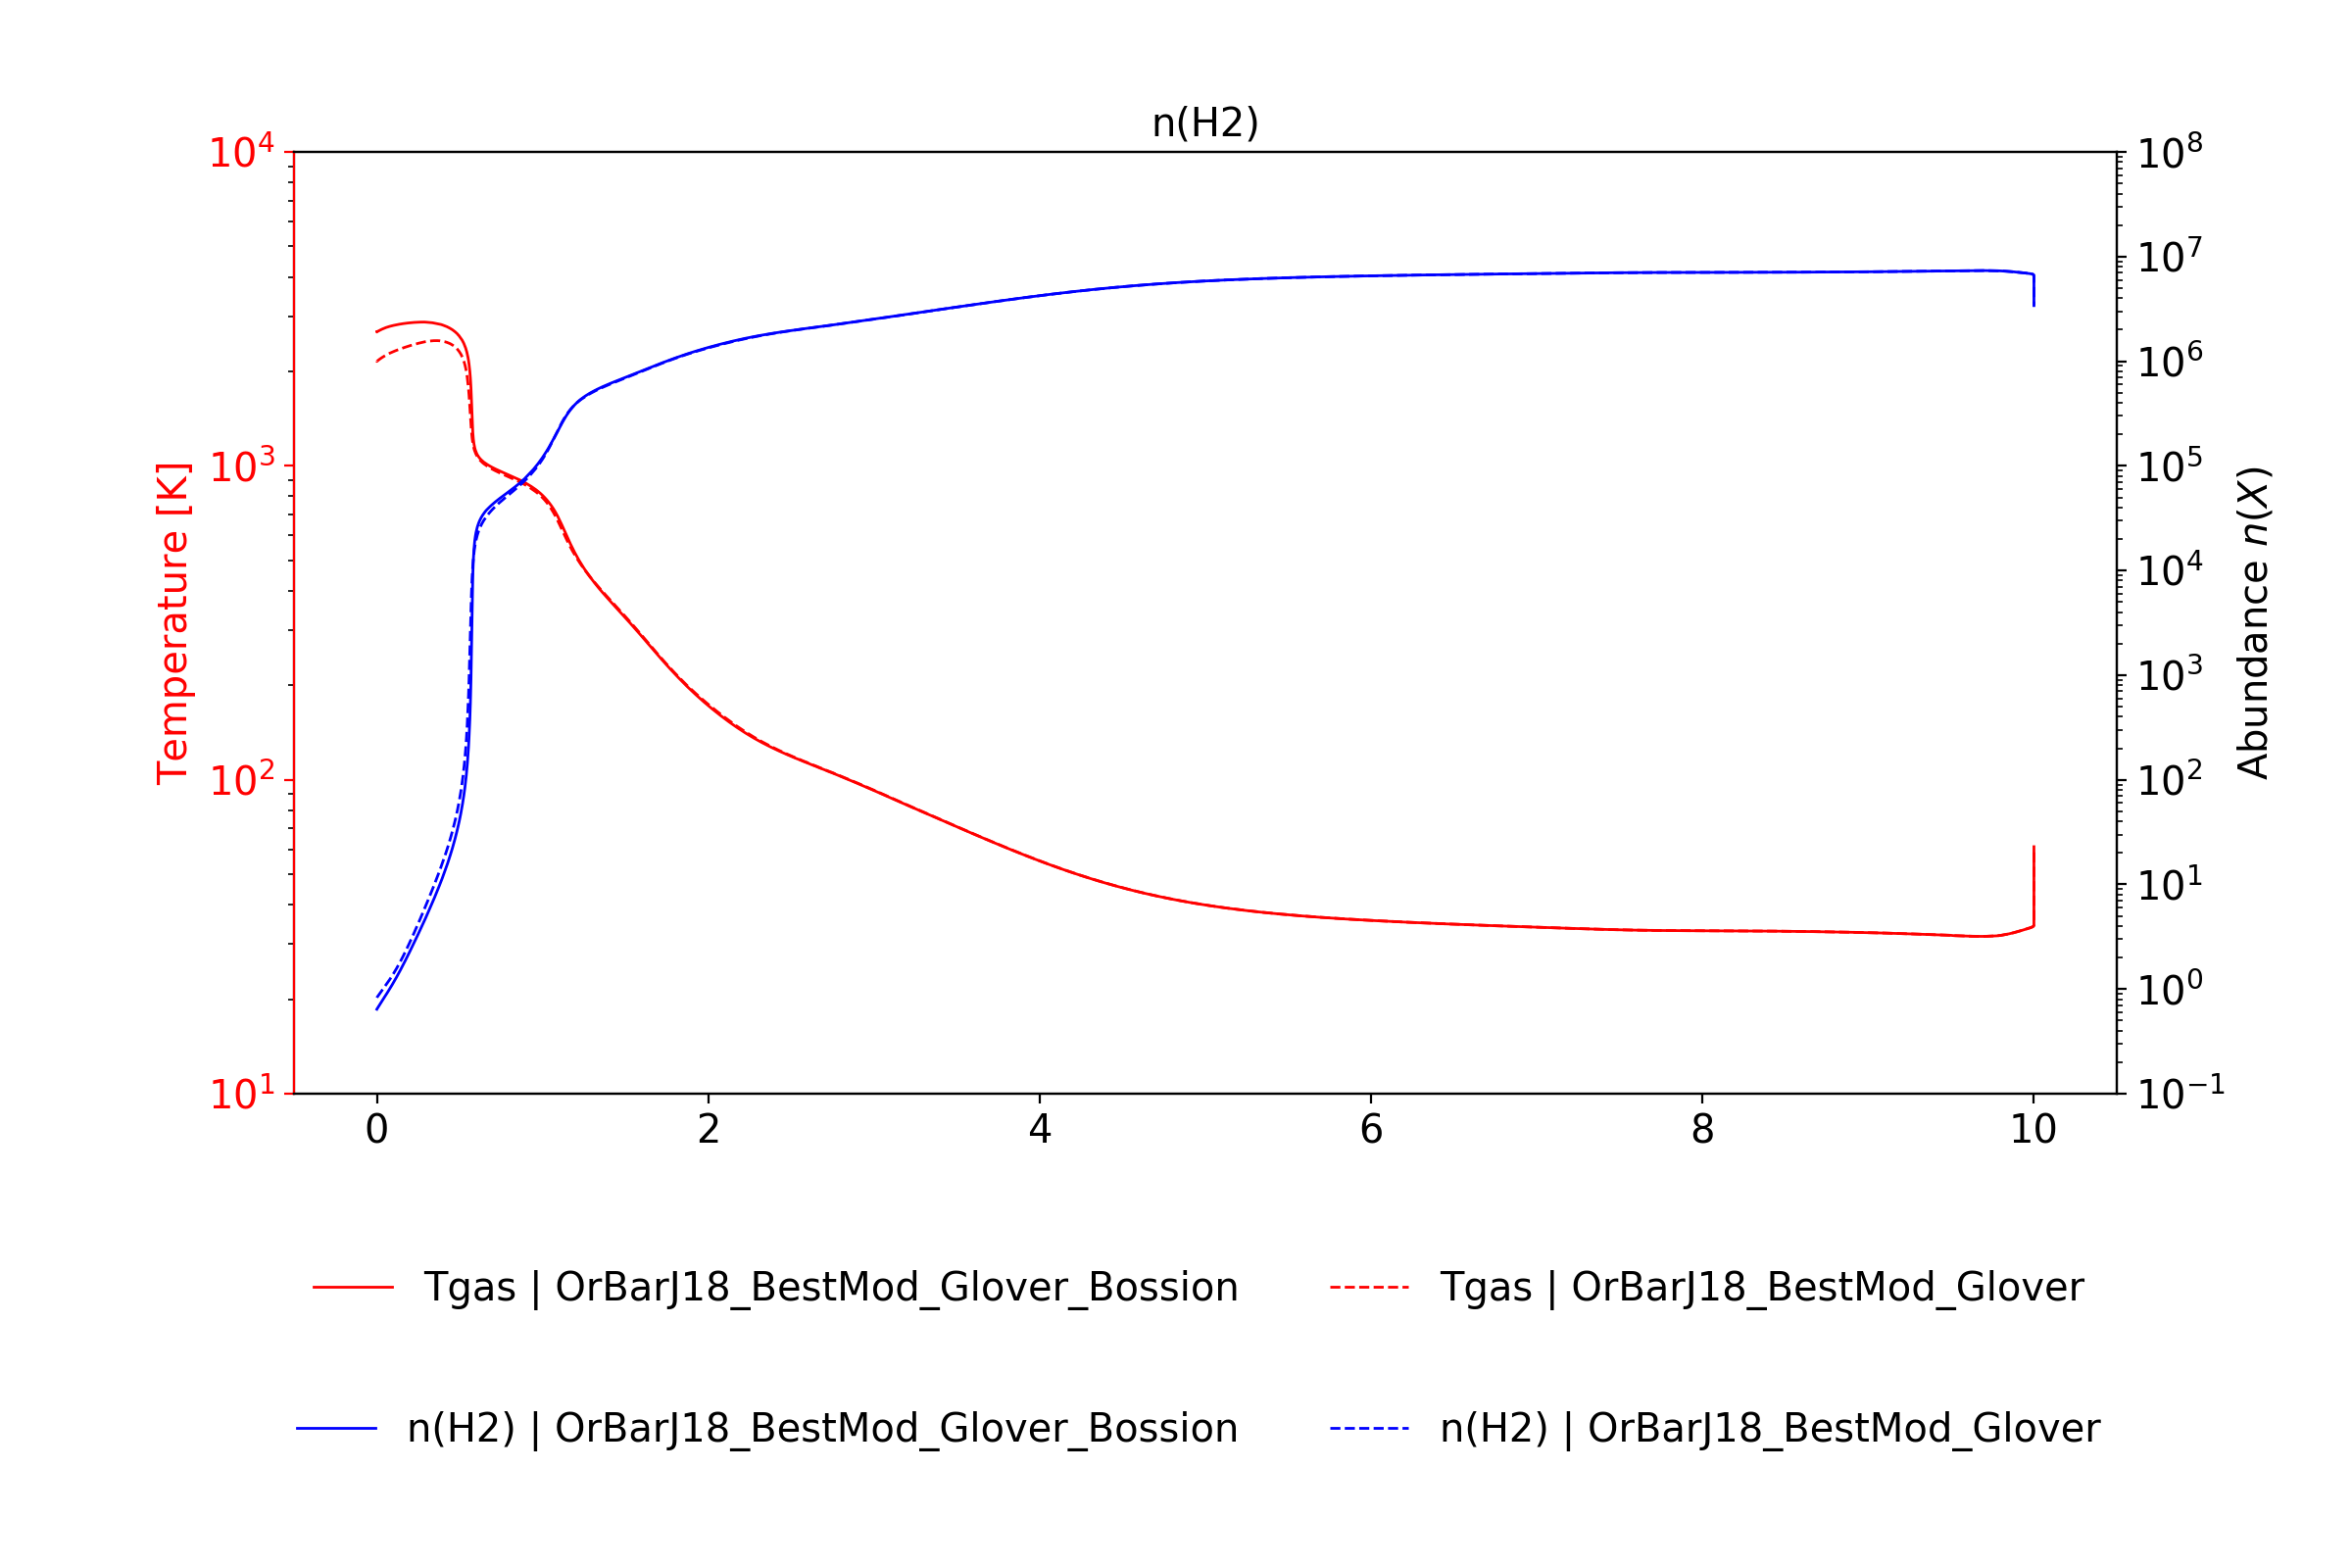
\includegraphics[trim = {0 0 0 1.5cm},clip,width=1\textwidth]{figure/H2/GloverBossion/nT_comp_H2.png}
%         \caption{Profil de densité et température de $\mathrm{CO}$}
%     \end{subfigure}
%     \caption{Comparaison des raies d'émissions des traceurs $\mathrm{H}_2$ et $\mathrm{CO}$ entre les calculs avec ou sans Bossion}
%     \label{fig:H2:GloverBossion:emiss}
% \end{figure}

% \subsection{Utilisation des nouveaux taux de collisions (Glover)}
% \subsection{A la recherche de l'instabilité par $\mathrm{H}_2$}
% \subsubsection{Où le chauffage par $\mathrm{H}_2$ prédomine-t-il dans le nuage ?}

% On a choisit quelques modèles parmi l'ensemble des calculs de la version \unsept utilisant les nouveaux taux de collisions. Il s'agit toujours de modèles à densités constantes. Ils sont symbolisé par des cercles pleins (en noirs) sur la figure \ref{fig:H2:mapGloverBossion:Gmax} et ont des conditions physiques différentes. On trace leurs profils de température à travers le nuage et l'on observe plusieurs choses (\autoref{fig:H2:mapGloverBossion:profilTx}) :  

% \begin{figure}[h!]
%     \centering
%     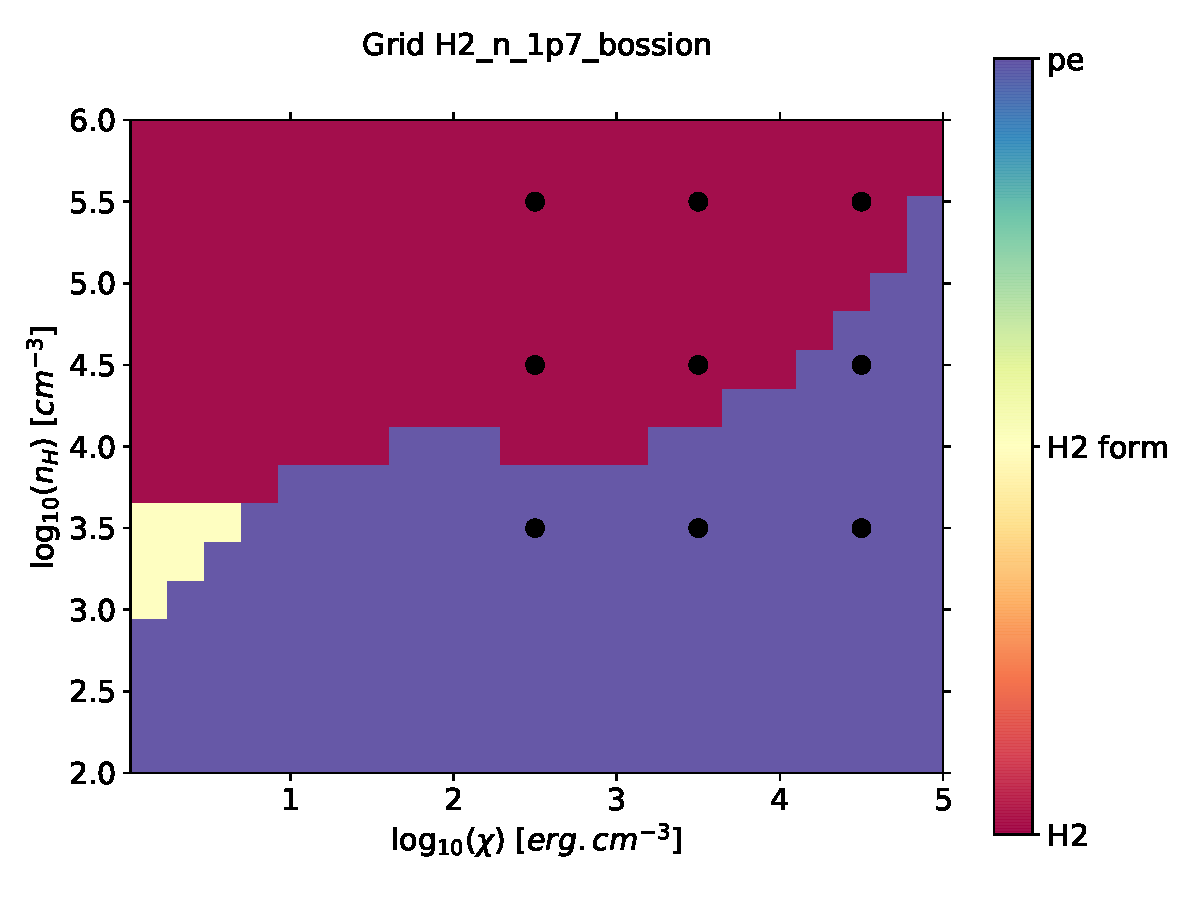
\includegraphics[width = 0.6\textwidth]{figure/H2/grid_gloverBossion/mapGmax_cross.pdf}
%     \caption{}
%     \label{fig:H2:mapGloverBossion:Gmax}
% \end{figure}


% \begin{itemize}
%     \item On voit (d) que la température au bord du nuage augmente pour les fort champs de rayonnement et que cette tendance est moins vraie (c) si le chauffage par $\mathrm{H}_2$ cesse de prédominer en bord de nuage (\ref{fig:H2:mapGloverBossion:Gmax}). Il vient un $\chi$ où la température augmente de manière raide à l'entrée du nuage moléculaire (a - $n_H = 10^{3.5}$ et $\chi = 10^{4.5}$). Je présume que c'est la recombinaison sur les grains qui est accélérée par le début de formation de $\mathrm{H}_2$ mais A VERIFIER. Comparer les $\Gamma$ et $\Lambda$ en fonction de la profondeur du nuage pour quelques modèles qui nous intéresse.
%     \item Si l'on se place à grand $\chi$ (b) le chauffage par $\mathrm{H}_2$ commence à prédominer en bord de nuage et on voit qu'il efface l'augmentation de température devant la partie moléculaire à mesure que le nuage devient dense. De même, en comparant (a) et (c), la recombinaison des grains s'intensifie avec le champs de rayonnement.
%     \item A forte densité (d) il apparaît un petit plateau après la transition $\mathrm{H}/\mathrm{H}_2$ : est ce que cela est du à l'effet photoélectrique ? pourrait il exciter d'avantage les raies du H2 ? On a vu avant qu'elle pouvait être du au chauffage par réactions chimiques qui devenait important car Glover tue la dissociation du H2. Et si l'on tracait ce T à cet endroit du nuage dans l'espace des paramètres. Peut être que l'on verrait aussi un bistabilité ? (première fois ou le gradient de T est minimale après la transition)
%     \item La température de la transition ne change pas d'un poil avec $\chi$ mais bouge avec la densité. Un fort champ de rayonnement ne fera que déplacer l'AV mais pas la température. Se comprend un peu car $\Gamma \propto n^2$ et $\Lambda \propto n $ mais pas toujours $\propto \chi$.
% \end{itemize}

% \begin{figure}[h!]
%     \centering
%     \begin{subfigure}[t]{0.49\textwidth} % "0.49" donne ici la largeur de l'image
%         \centering 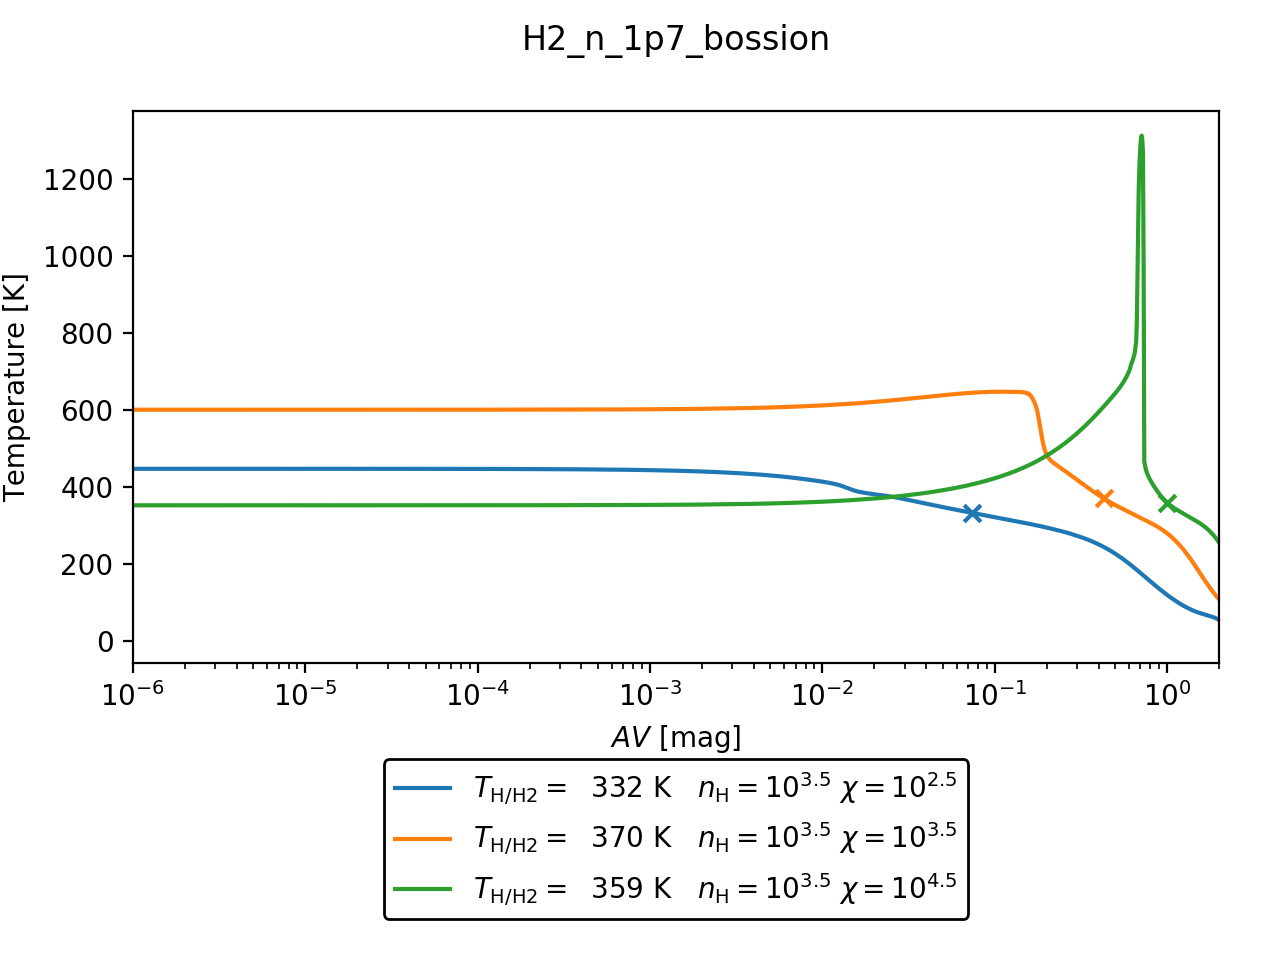
\includegraphics[trim = {0 0 0 0},clip,width=1\textwidth]{figure/H2/grid_gloverBossion/H2_n_1p7_bossion_d3p5r2p5_d3p5r3p5_d3p5r4p5.png} 
%         \caption{}
%     \end{subfigure}
%     ~ 
%     \begin{subfigure}[t]{0.49\textwidth}
%         \centering 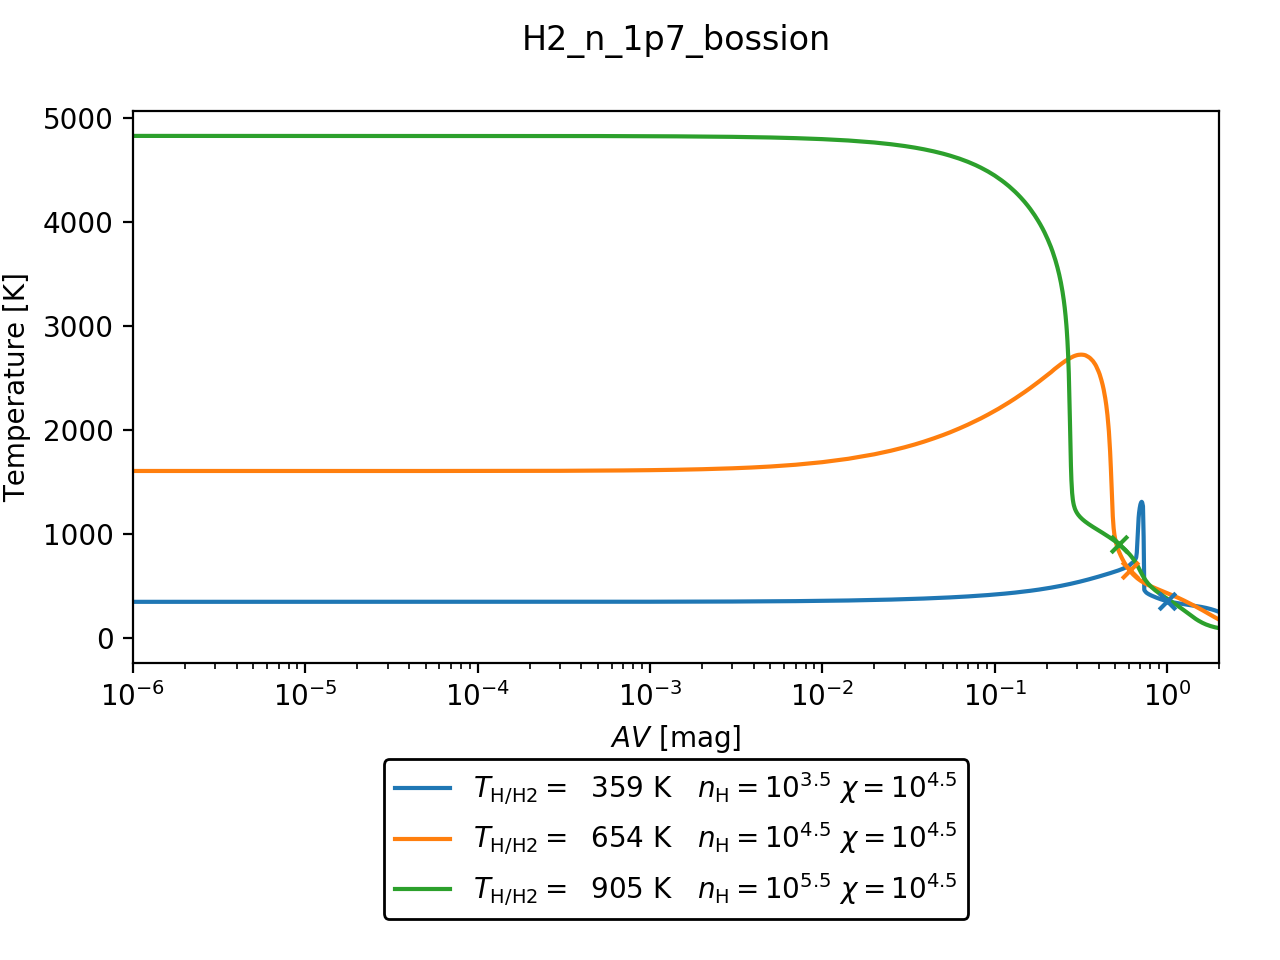
\includegraphics[trim = {0 0 0 0},clip,width=1\textwidth]{figure/H2/grid_gloverBossion/H2_n_1p7_bossion_d3p5r4p5_d4p5r4p5_d5p5r4p5.png}
%         \caption{}
%     \end{subfigure}

%     \centering
%     \begin{subfigure}[t]{0.49\textwidth} % "0.49" donne ici la largeur de l'image
%         \centering 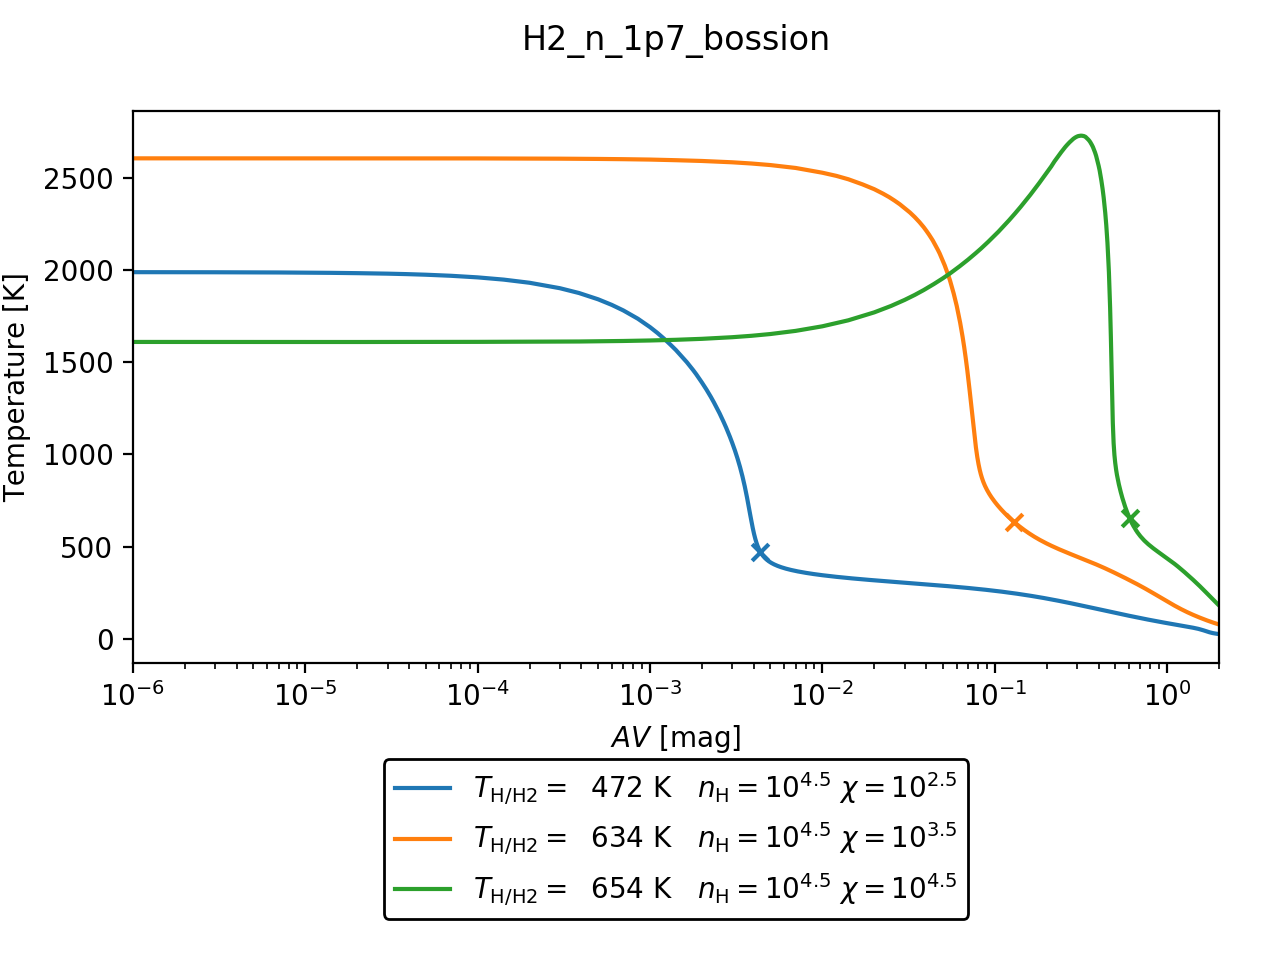
\includegraphics[trim = {0 0 0 0},clip,width=1\textwidth]{figure/H2/grid_gloverBossion/H2_n_1p7_bossion_d4p5r2p5_d4p5r3p5_d4p5r4p5.png} 
%         \caption{}
%     \end{subfigure}
%     ~ 
%     \begin{subfigure}[t]{0.49\textwidth}
%         \centering 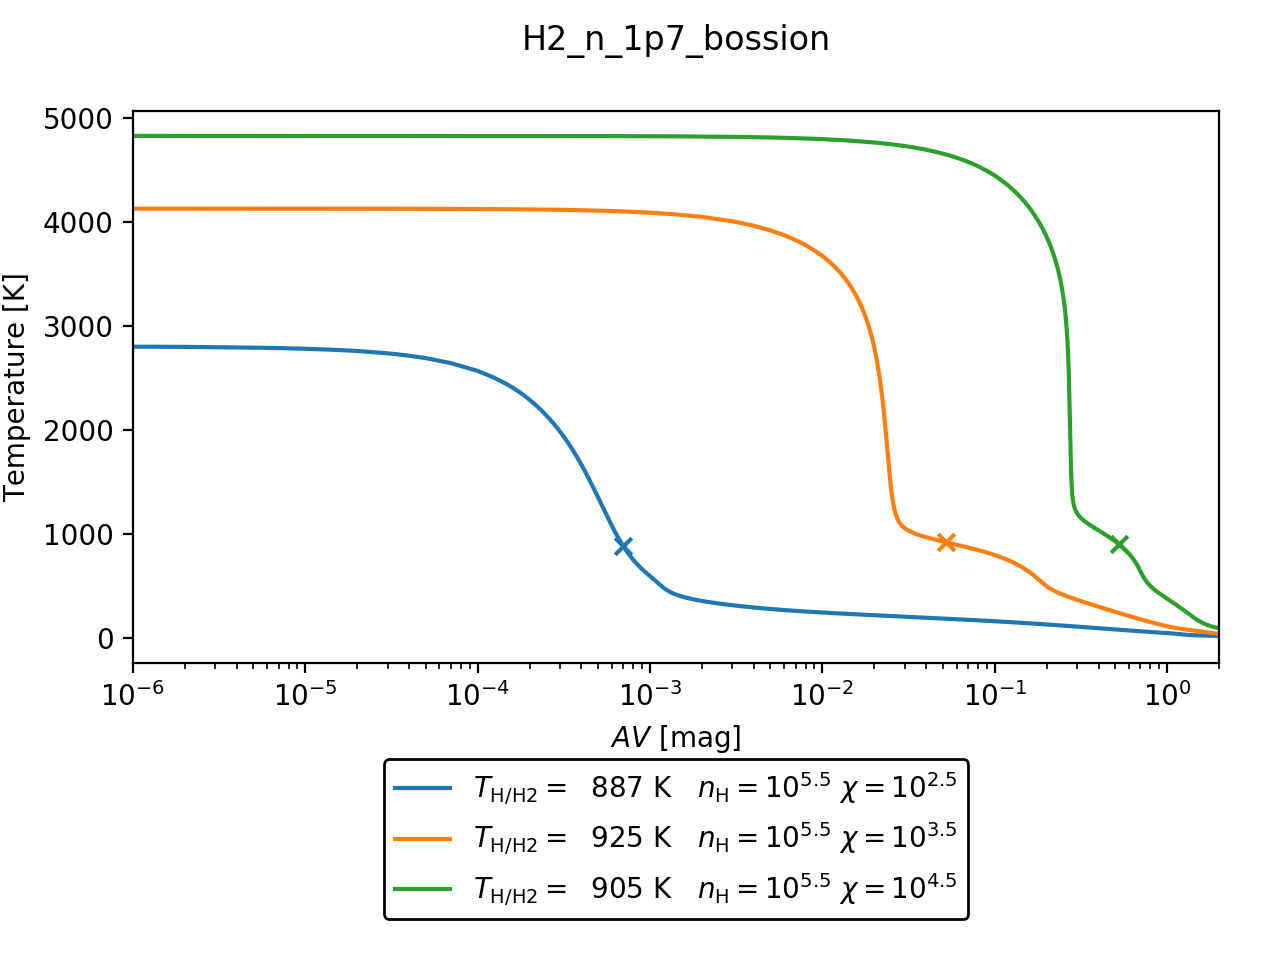
\includegraphics[trim = {0 0 0 0},clip,width=1\textwidth]{figure/H2/grid_gloverBossion/H2_n_1p7_bossion_d5p5r2p5_d5p5r3p5_d5p5r4p5.png} 
%         \caption{}
%     \end{subfigure}
%     \caption{Profil de températures pour différent modèles de la grille (Glover + Bossion). La croix indique la température de la transition $\mathrm{H}/\mathrm{H}_2$ : $n(\mathrm{H})=2n(\mathrm{H}_2)$.}
%     \label{fig:H2:mapGloverBossion:profilTx}
% \end{figure}

% \subsection{Dans quelles conditions le chauffage par $\mathrm{H}_2$ prédomine-t-il ?}

% On observe également la température de la transition $\mathrm{H}/\mathrm{H}_2$ dans l'espace des paramètres (\autoref{fig:H2:mapGloverBossion:mapTHH2}). La température ne dépend toujours pas de l'intensité du champs de rayonnements et on arrive encore à dépasser le plateau de $600K$. Cependant les nouveaux taux de collisions n'apportent rien.\newline 

% \begin{figure}[th!]
%     \centering
%     \begin{subfigure}[t]{0.49\textwidth} % "0.49" donne ici la largeur de l'image
%         \centering 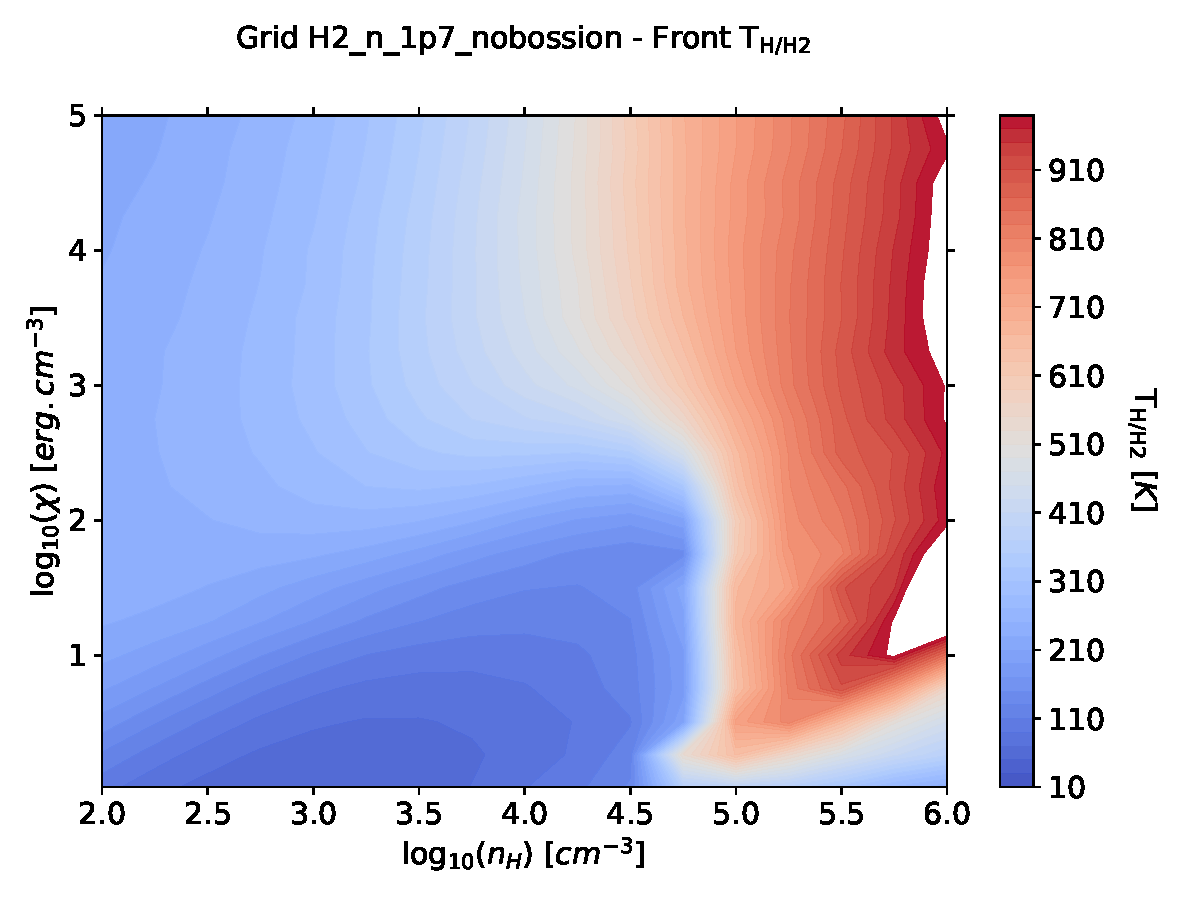
\includegraphics[trim = {0 0 0 0},clip,width=1\textwidth]{figure/H2/grid_glovernoBossion/HH2_T_Franck.pdf}
%         \caption{}
%     \end{subfigure}
%     ~ 
%     \begin{subfigure}[t]{0.49\textwidth}
%         \centering 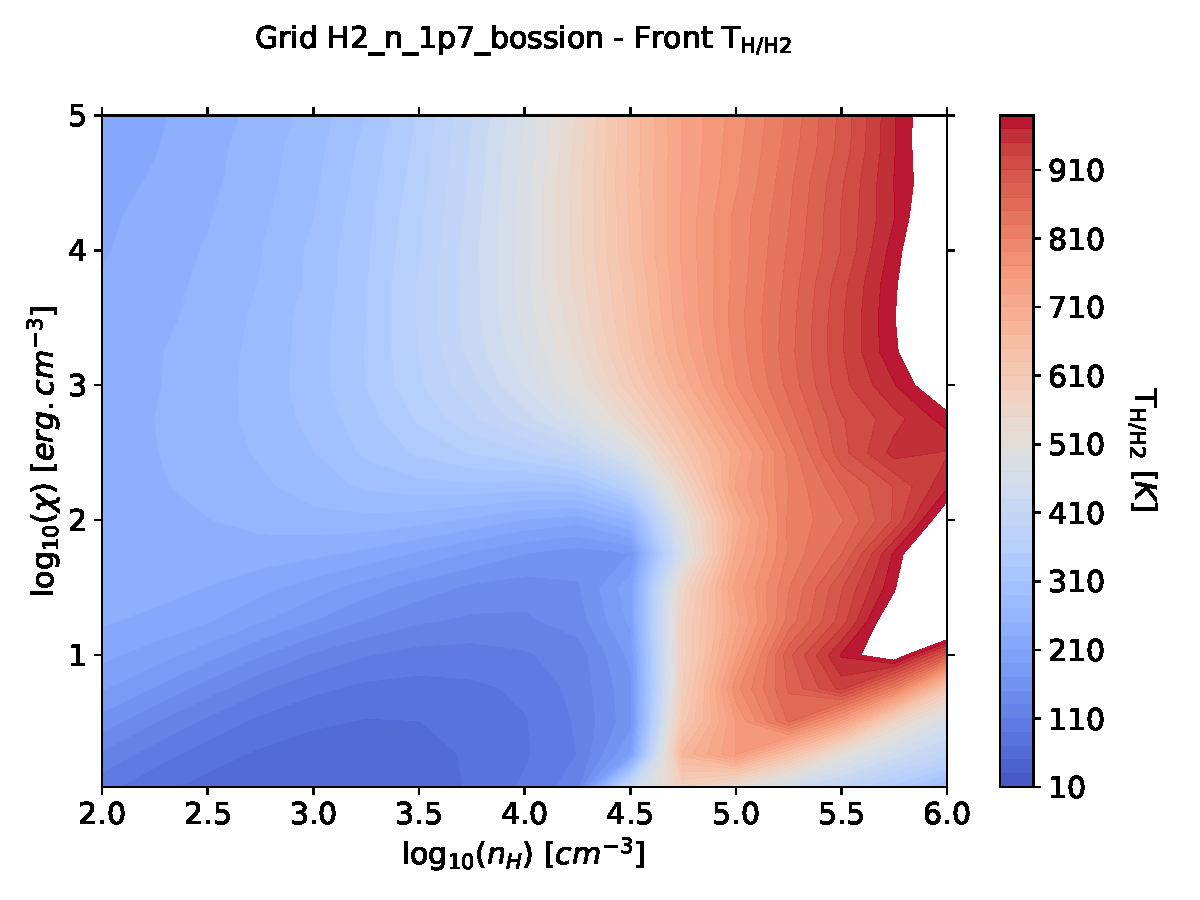
\includegraphics[trim = {0 0 0 0},clip,width=1\textwidth]{figure/H2/grid_gloverBossion/HH2_T_Franck.pdf}
%         \caption{}
%     \end{subfigure}
%     \caption{Carte de températures de la transition $\mathrm{H}/\mathrm{H}_2$ : $n(\mathrm{H})=2n(\mathrm{H}_2)$ avec (a) ou sans (b) les niveaux de Bossion (Glover)}
%     \label{fig:H2:mapGloverBossion:mapTHH2}
% \end{figure}

% \underline{Conclusion partielle :}On voit que le chauffage par $\mathrm{H}_2$ concerne les régions denses et impactent principalement les bords atomiques. Or c'est si l'on chauffait l'entrée du nuage que l'on pourrait espérer observer les changements. Il faudrait regarder les diagrammes d'excitations de quelques espèces comme $\mathrm{H}_2$ ou $\mathrm{CO}$. On se pose également une question sur l'impact de la raideur de la transition sur la température (\autoref{fig:H2:mapGloverBossion:smooth}) : dans certains cas, la transition se fait pour des gaz encore chaud ce qui signifie que l'on pourrait voir des raies plus excitées. Dans quelles conditions ces phénomènes ont ils lieux ? Est ce que cela a un impact sur les raies ? 
% (Sternberg 2014) Enfin on n'a pas observé les instabilités que pouvait provoquer le $\mathrm{H}_2$. Tracer quelques courbes de chauffages et refroidissements pour différent modèles (là le gradient de Tmax) est maximale par exemple. On observait également mieux l'instabilité sur des modèles isobares : faire une petite grille. 
% Pour avancer sur cette histoire de chauffage par réaction chimiqie : tracer $\max_{AV} \Gamma_{ch}/\Gamma_{tot}$ dans l'espace des paramètres et le $(argmax_{AV}  \Gamma_{ch}/\Gamma_{tot})/AV_{HH2}$ qui est lié également au $\mathrm{H}_2$ par la réaction avec le $\mathrm{CH}^+$

% \begin{figure}[th!]
%         \centering 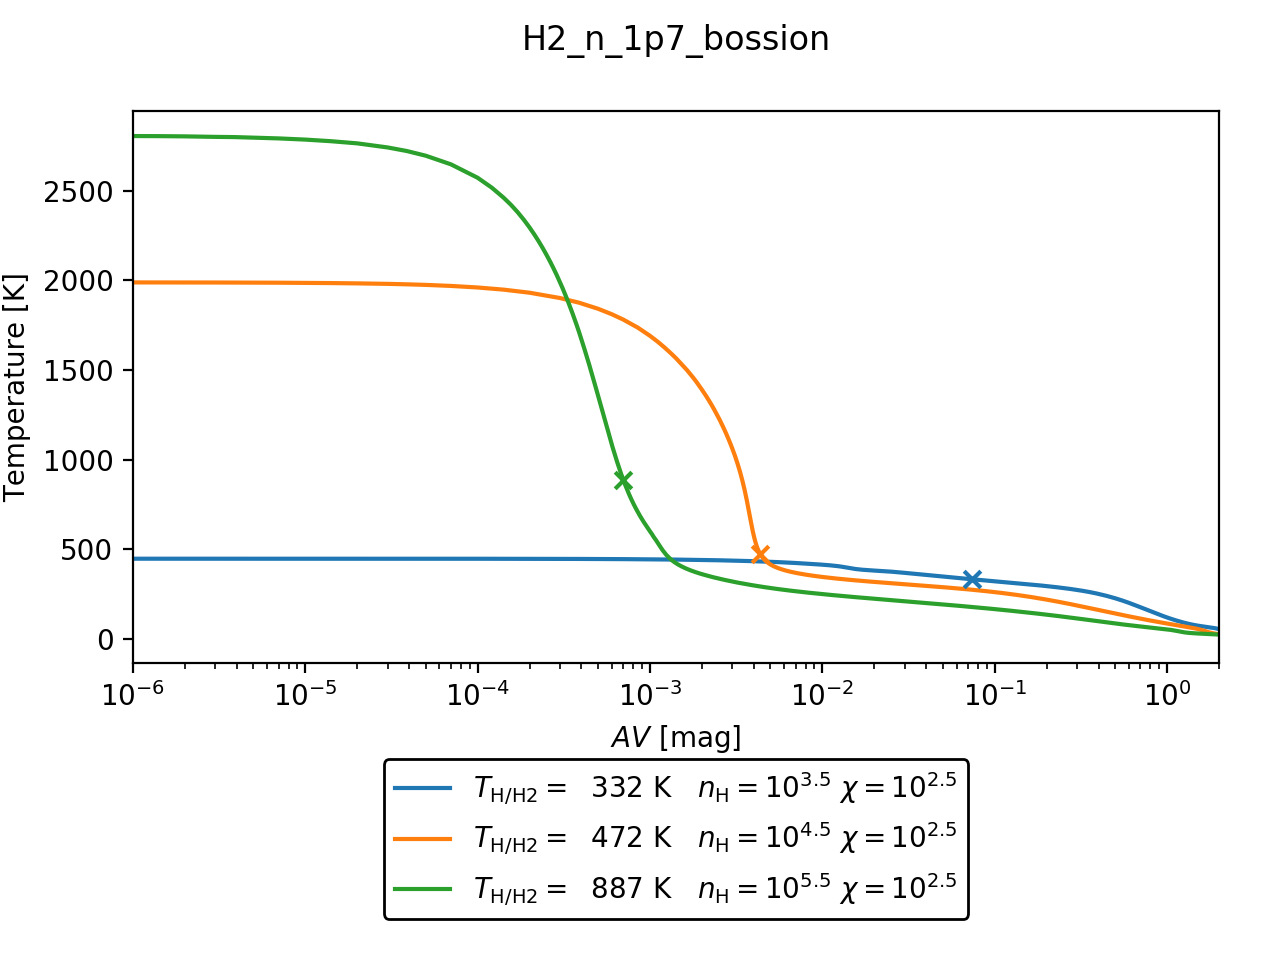
\includegraphics[trim = {0 0 0 0},clip,width=0.5\textwidth]{figure/H2/grid_gloverBossion/H2_n_1p7_bossion_d3p5r2p5_d4p5r2p5_d5p5r2p5.png}
%         \caption{Profils de températures de différents modèles de la grille (Glover + Bossion)}
%         \label{fig:H2:mapGloverBossion:smooth}
% \end{figure}

% \subsubsection{Dans quelles conditions peut on voir une instabilité ?}
% \subsubsection{Quel est l'impact sur les raies des traceurs ?}


% \subsubsection{Bonus}